\ifnpas


\begin{figure}[htbp]
\centering
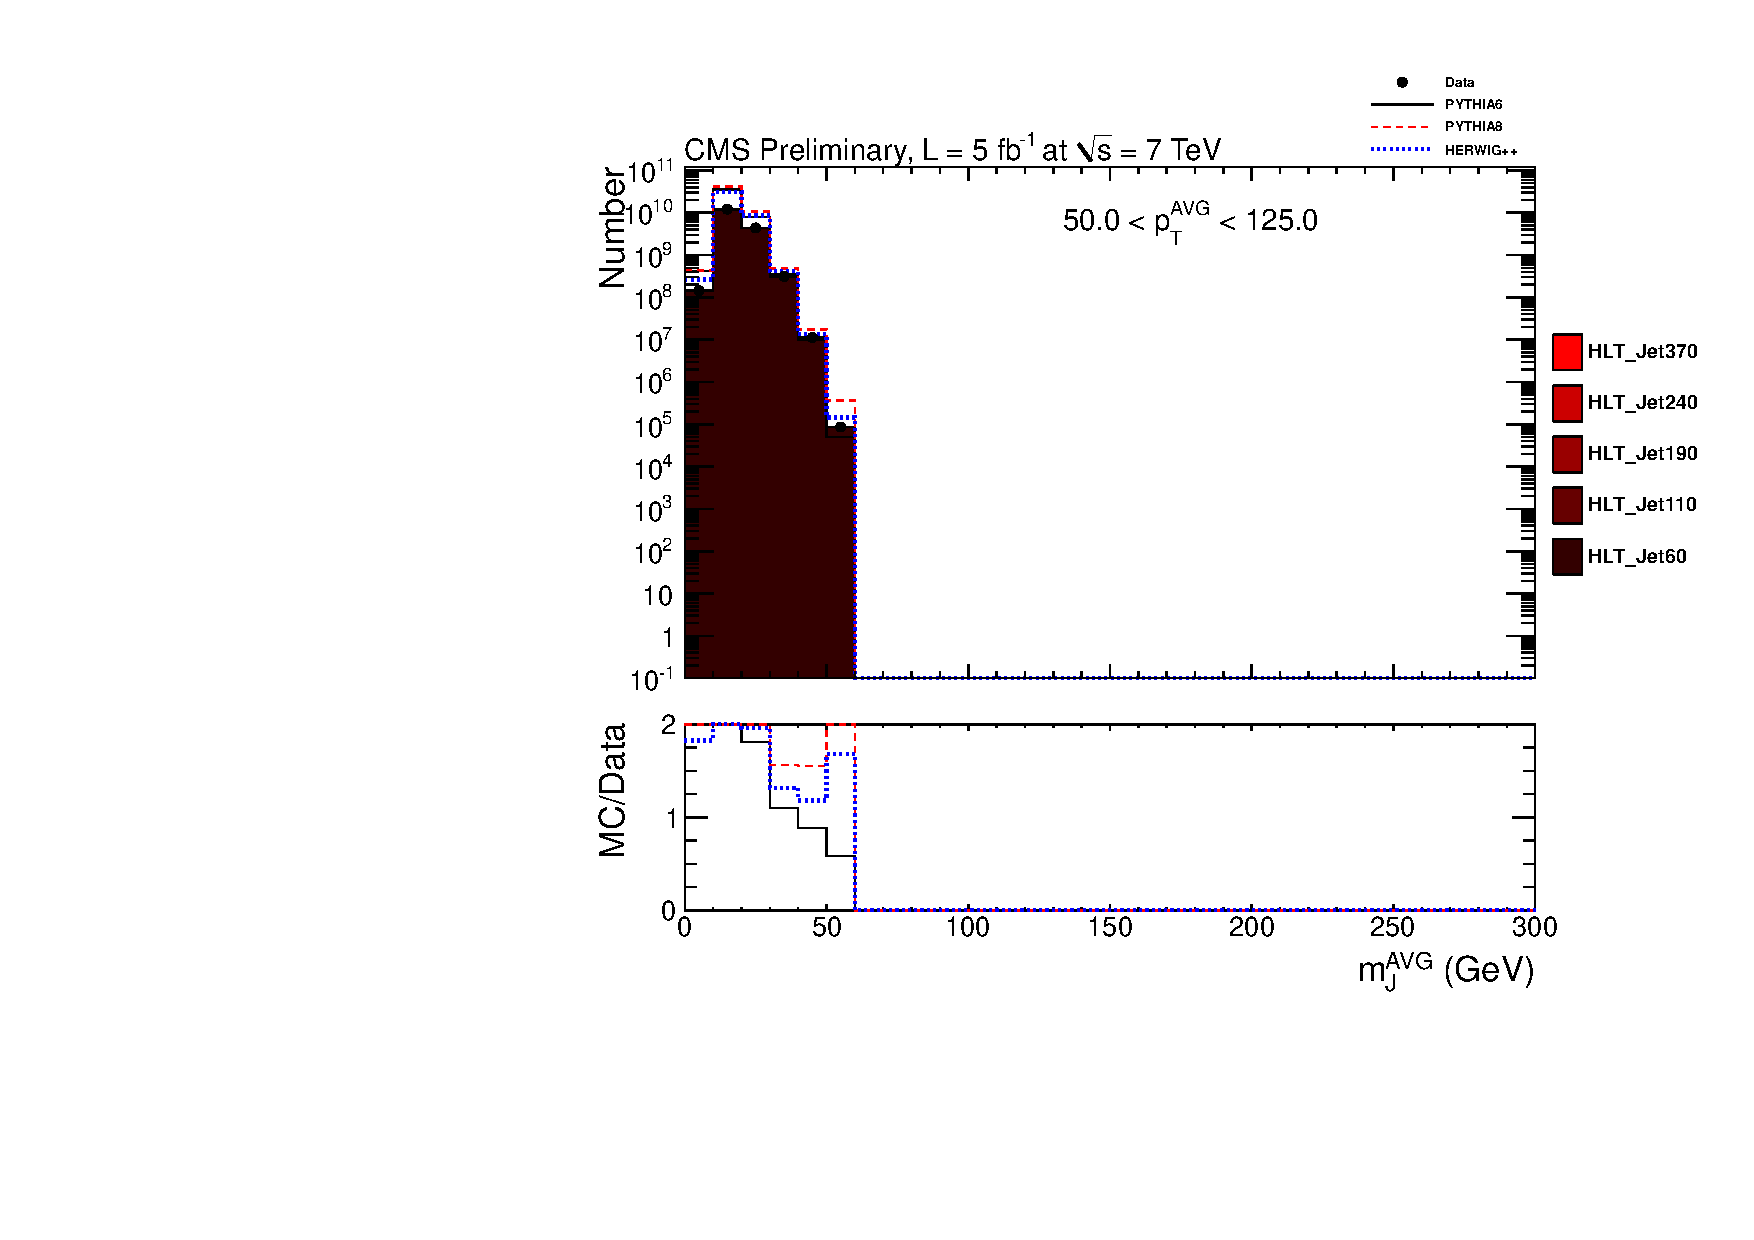
\includegraphics[width=0.95\textwidth]{figs/histAK7MjetVsPtAvg_rawDataMCComparisons_stacktrigs_pt_1}
for $50.0 < \pt^{AVG} < 125.0$ \GeVc. The data are shown in black points.
The simulated distribution from \PYTHIA is shown in solid black, 
the from \PYTHIAEIGHT in dashed red, and from \HERWIG in dotted blue. 
The bottom frame shows the ratio of the simulated distribution
to the distribution from data. The various trigger contributions are shown in shades of red.
\label{figs:histAK7MjetVsPtAvg_rawDataMCComparisons_stacktrigs_pt_1}}
\end{figure}


\begin{figure}[htbp]
\centering
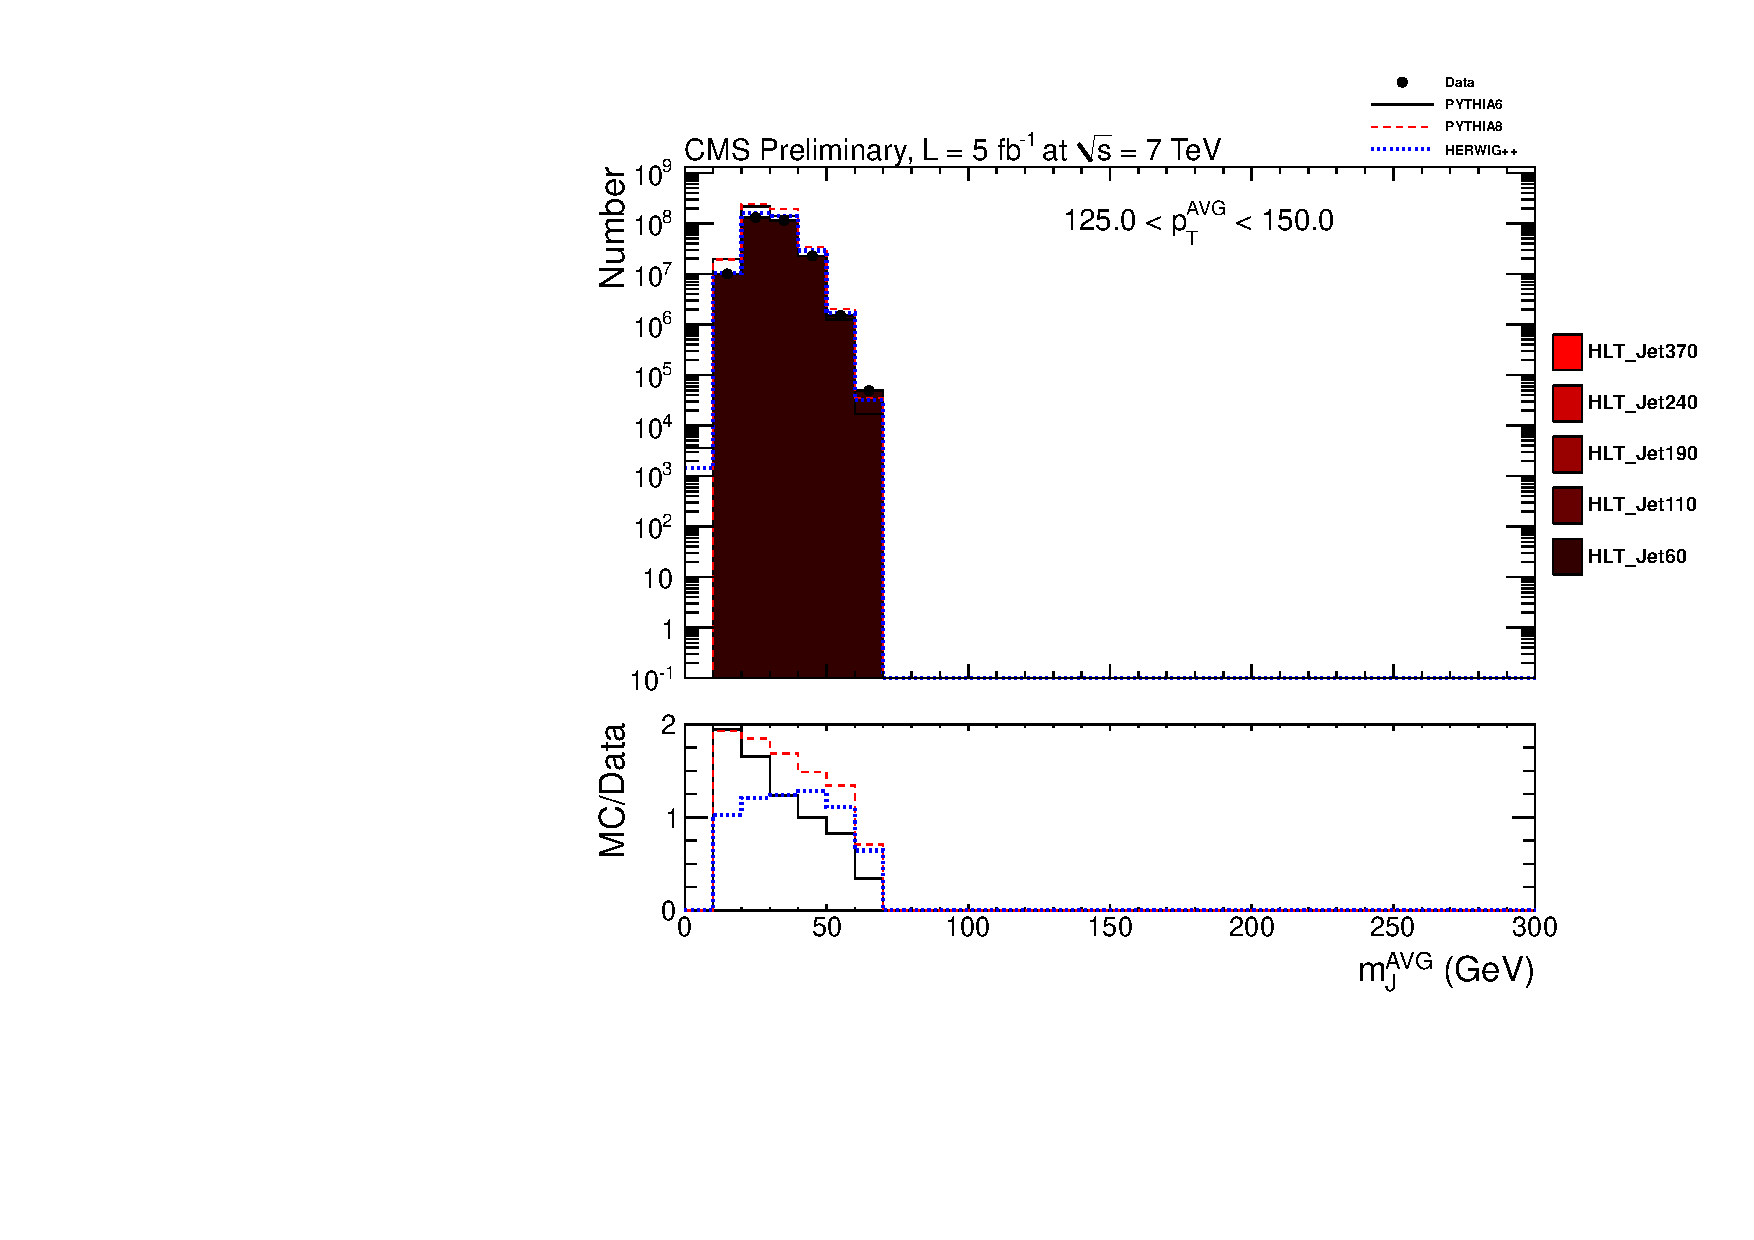
\includegraphics[width=0.95\textwidth]{figs/histAK7MjetVsPtAvg_rawDataMCComparisons_stacktrigs_pt_2}
\caption{Detector-level distributions of the jet mass for AK7 jets,
for $125.0 < \pt^{AVG} < 150.0$ \GeVc. The data are shown in black points.
The simulated distribution from \PYTHIA is shown in solid black, 
the from \PYTHIAEIGHT in dashed red, and from \HERWIG in dotted blue. 
The bottom frame shows the ratio of the simulated distribution
to the distribution from data. The various trigger contributions are shown in shades of red.
\label{figs:histAK7MjetVsPtAvg_rawDataMCComparisons_stacktrigs_pt_2}}
\end{figure}



\begin{figure}[htbp]
\centering
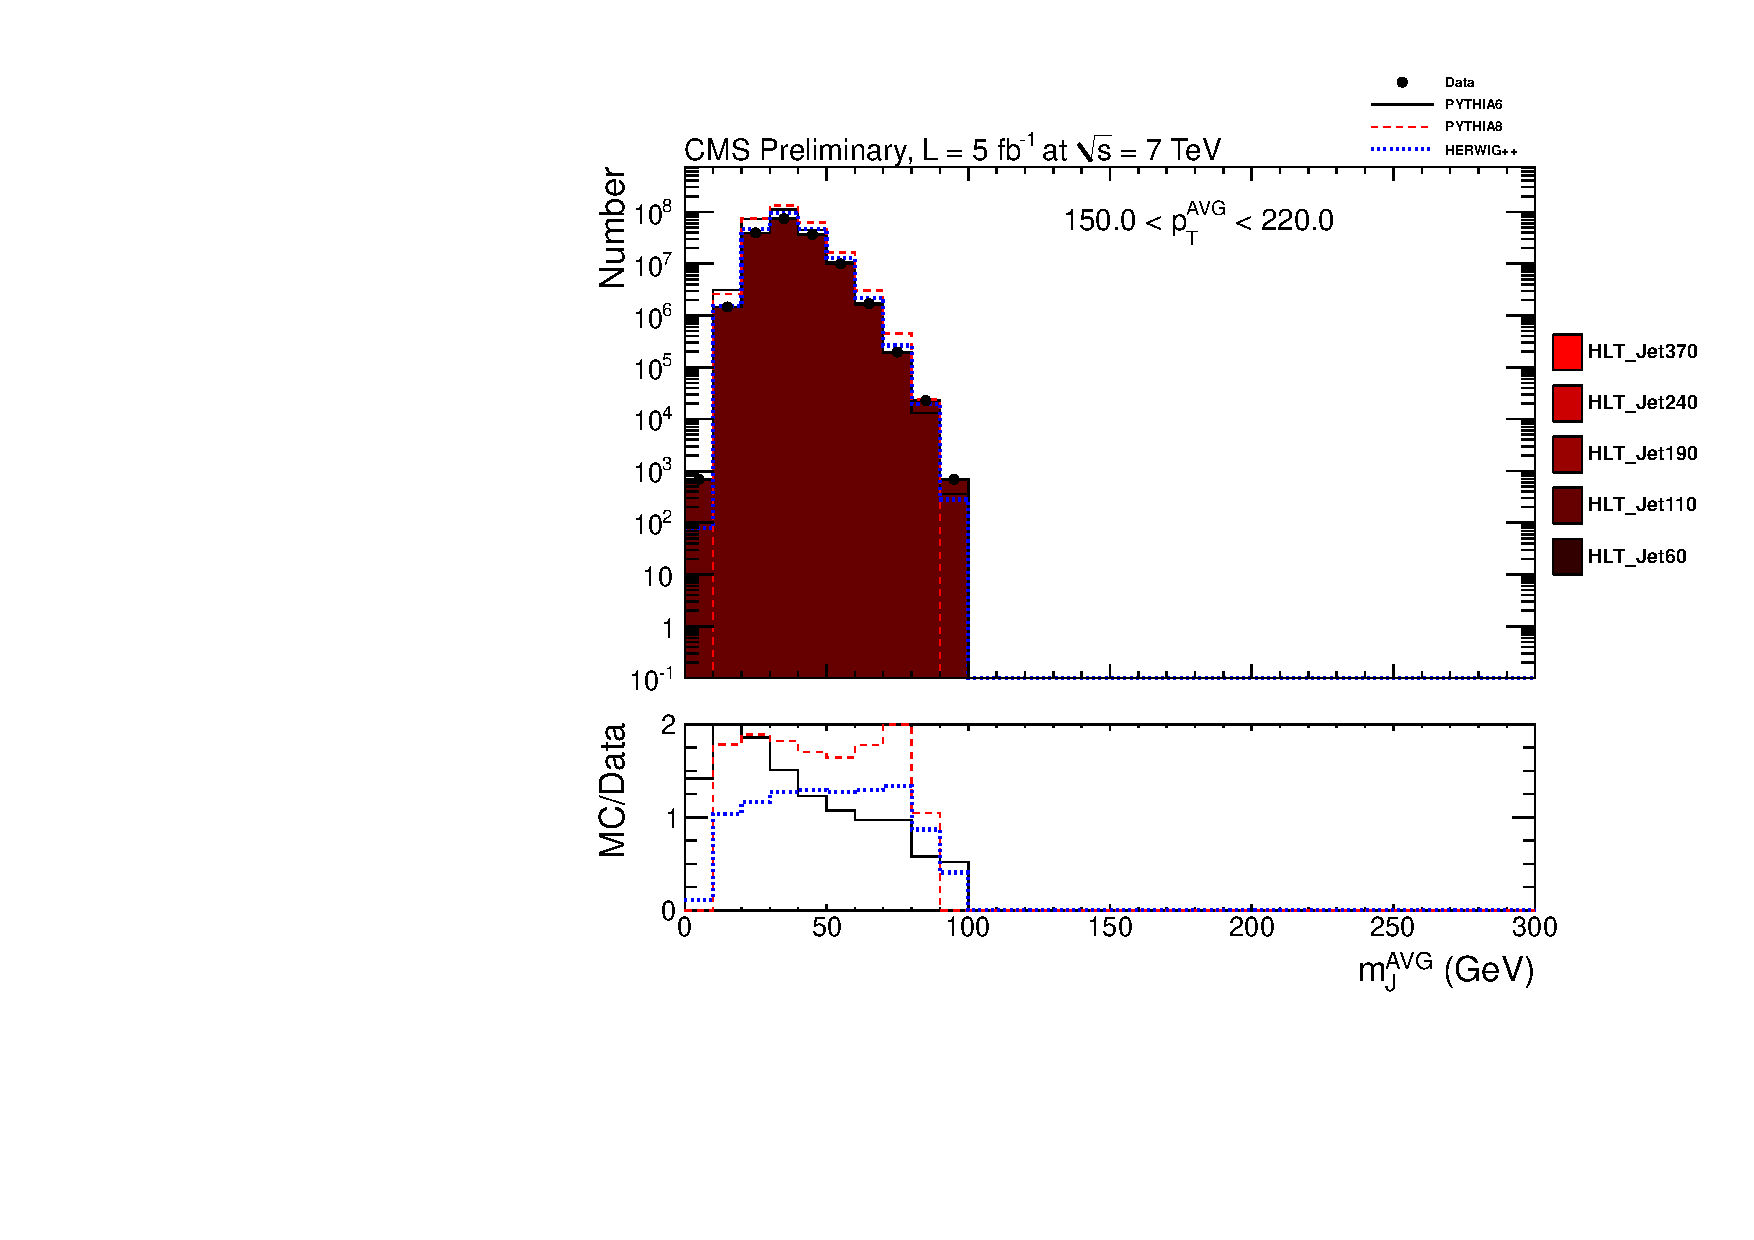
\includegraphics[width=0.95\textwidth]{figs/histAK7MjetVsPtAvg_rawDataMCComparisons_stacktrigs_pt_3}
\caption{Detector-level distributions of the jet mass for AK7 jets,
for $150.0 < \pt^{AVG} < 220.0$ \GeVc. The data are shown in black points.
The simulated distribution from \PYTHIA is shown in solid black, 
the from \PYTHIAEIGHT in dashed red, and from \HERWIG in dotted blue. 
The bottom frame shows the ratio of the simulated distribution
to the distribution from data. The various trigger contributions are shown in shades of red.
\label{figs:histAK7MjetVsPtAvg_rawDataMCComparisons_stacktrigs_pt_3}}
\end{figure}



\begin{figure}[htbp]
\centering
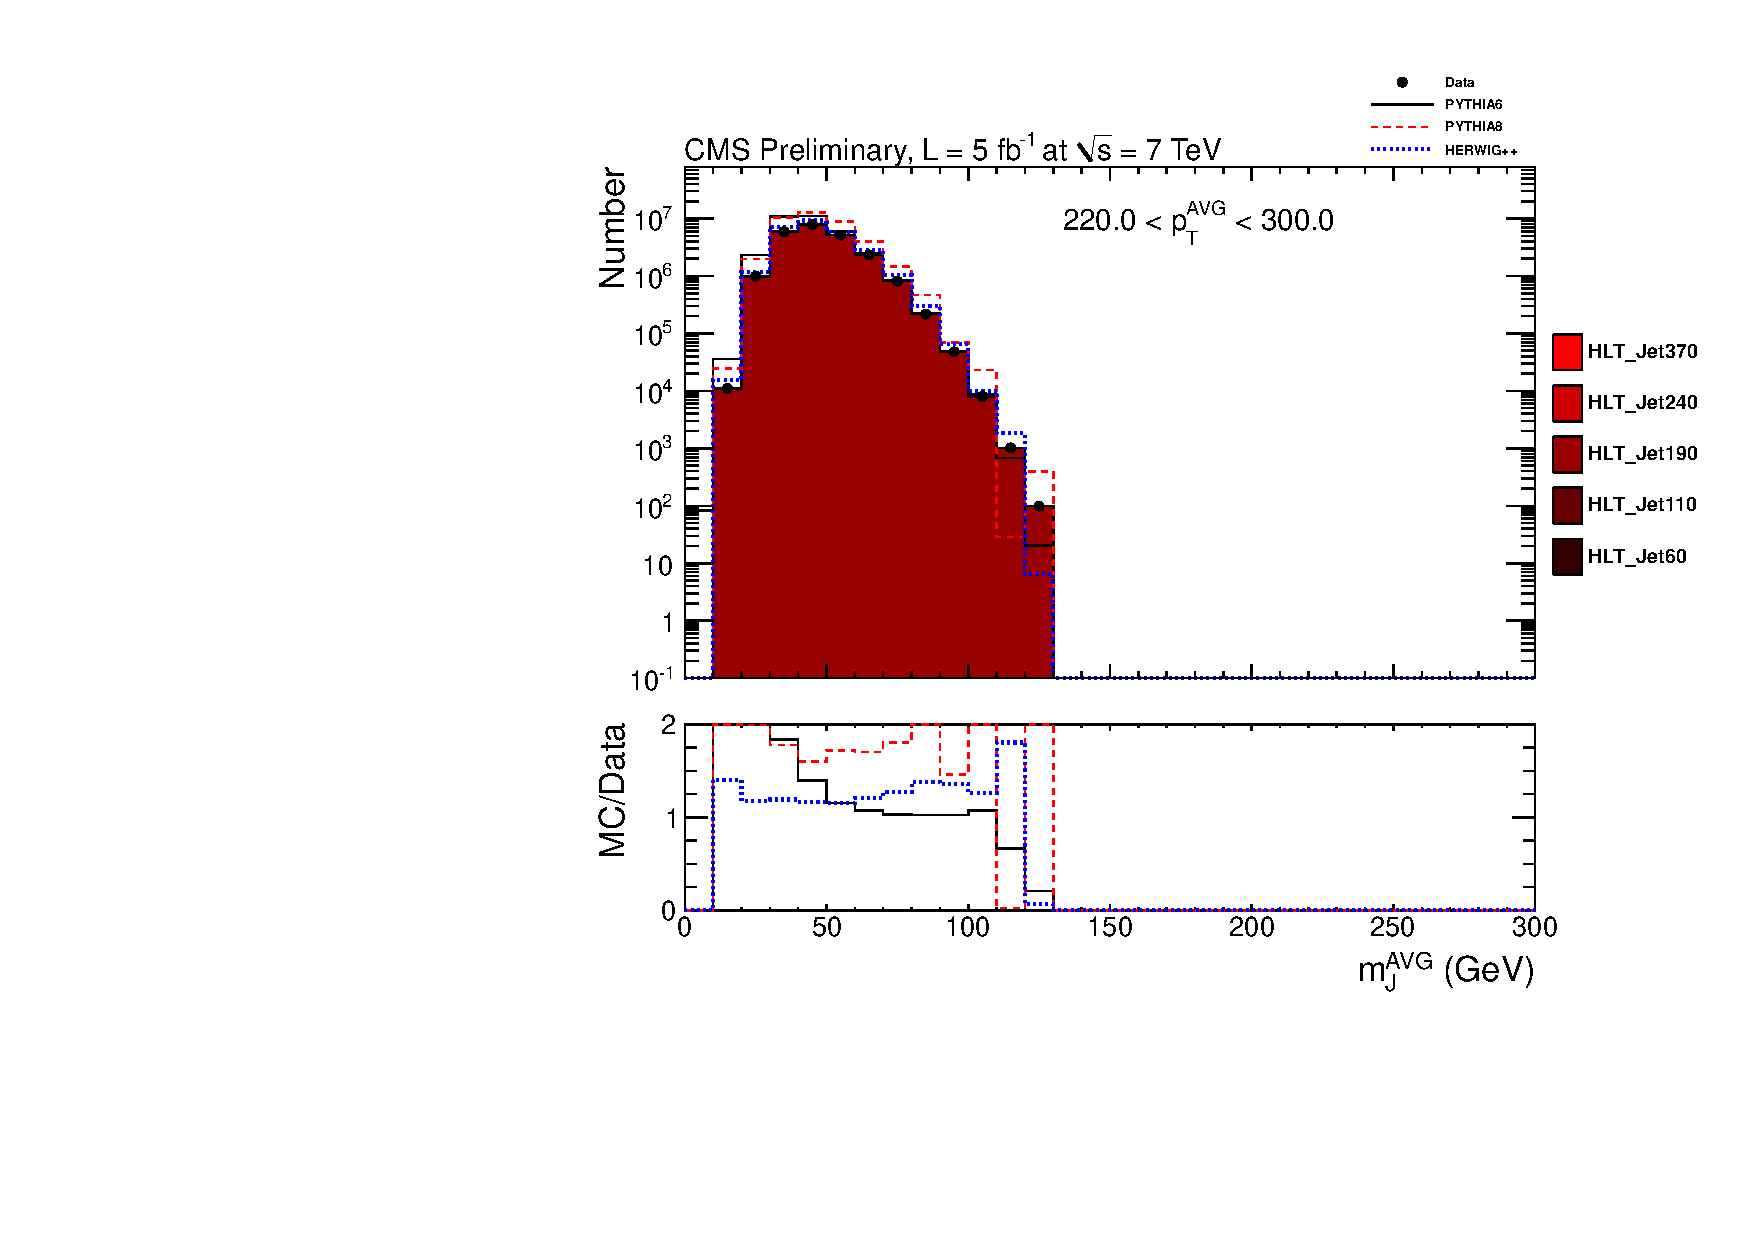
\includegraphics[width=0.95\textwidth]{figs/histAK7MjetVsPtAvg_rawDataMCComparisons_stacktrigs_pt_4}
\caption{Detector-level distributions of the jet mass for AK7 jets,
for $220.0 < \pt^{AVG} < 300.0$ \GeVc. The data are shown in black points.
The simulated distribution from \PYTHIA is shown in solid black, 
the from \PYTHIAEIGHT in dashed red, and from \HERWIG in dotted blue. 
The bottom frame shows the ratio of the simulated distribution
to the distribution from data. The various trigger contributions are shown in shades of red.
\label{figs:histAK7MjetVsPtAvg_rawDataMCComparisons_stacktrigs_pt_4}}
\end{figure}



\begin{figure}[htbp]
\centering
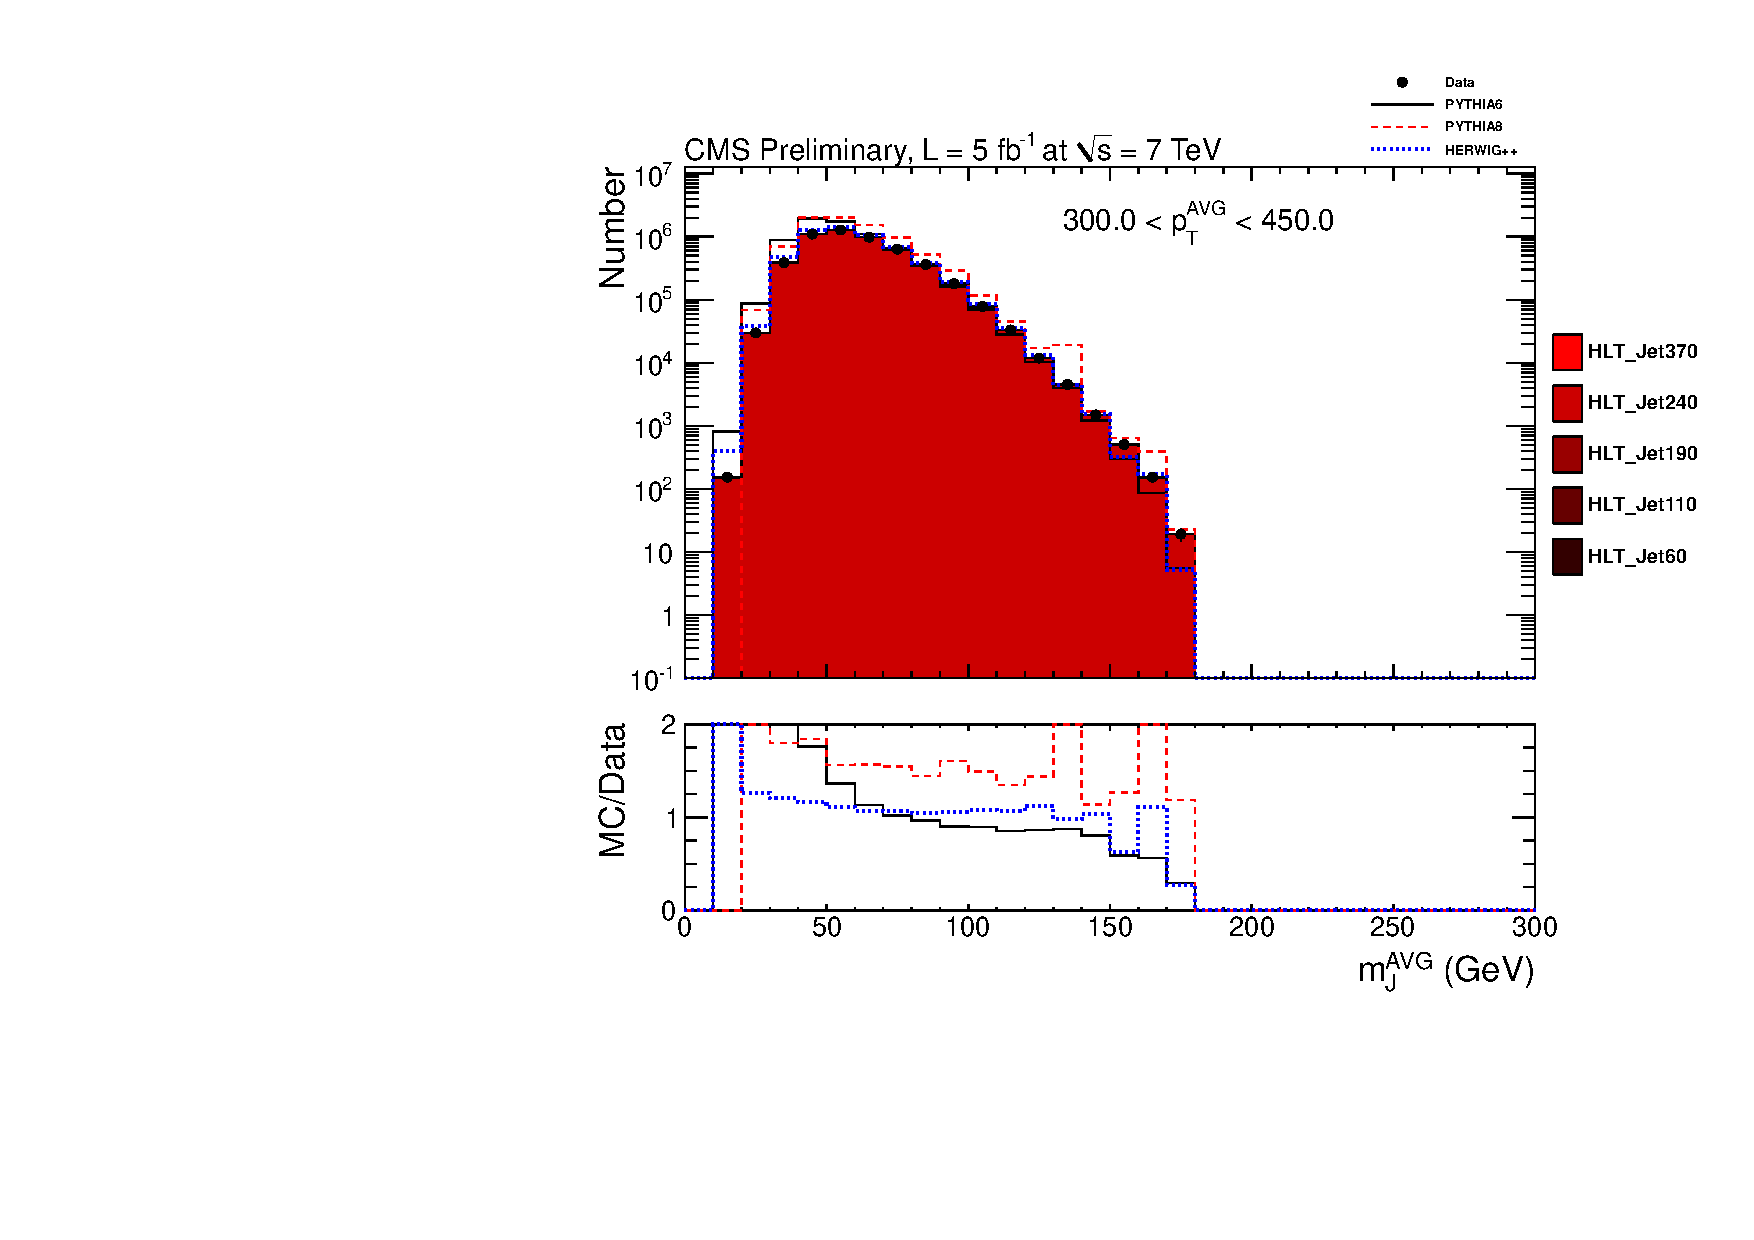
\includegraphics[width=0.95\textwidth]{figs/histAK7MjetVsPtAvg_rawDataMCComparisons_stacktrigs_pt_5}
\caption{Detector-level distributions of the jet mass for AK7 jets,
for $300.0 < \pt^{AVG} < 450.0$ \GeVc. The data are shown in black points.
The simulated distribution from \PYTHIA is shown in solid black, 
the from \PYTHIAEIGHT in dashed red, and from \HERWIG in dotted blue. 
The bottom frame shows the ratio of the simulated distribution
to the distribution from data. The various trigger contributions are shown in shades of red.
\label{figs:histAK7MjetVsPtAvg_rawDataMCComparisons_stacktrigs_pt_5}}
\end{figure}

\begin{figure}[htbp]
\centering
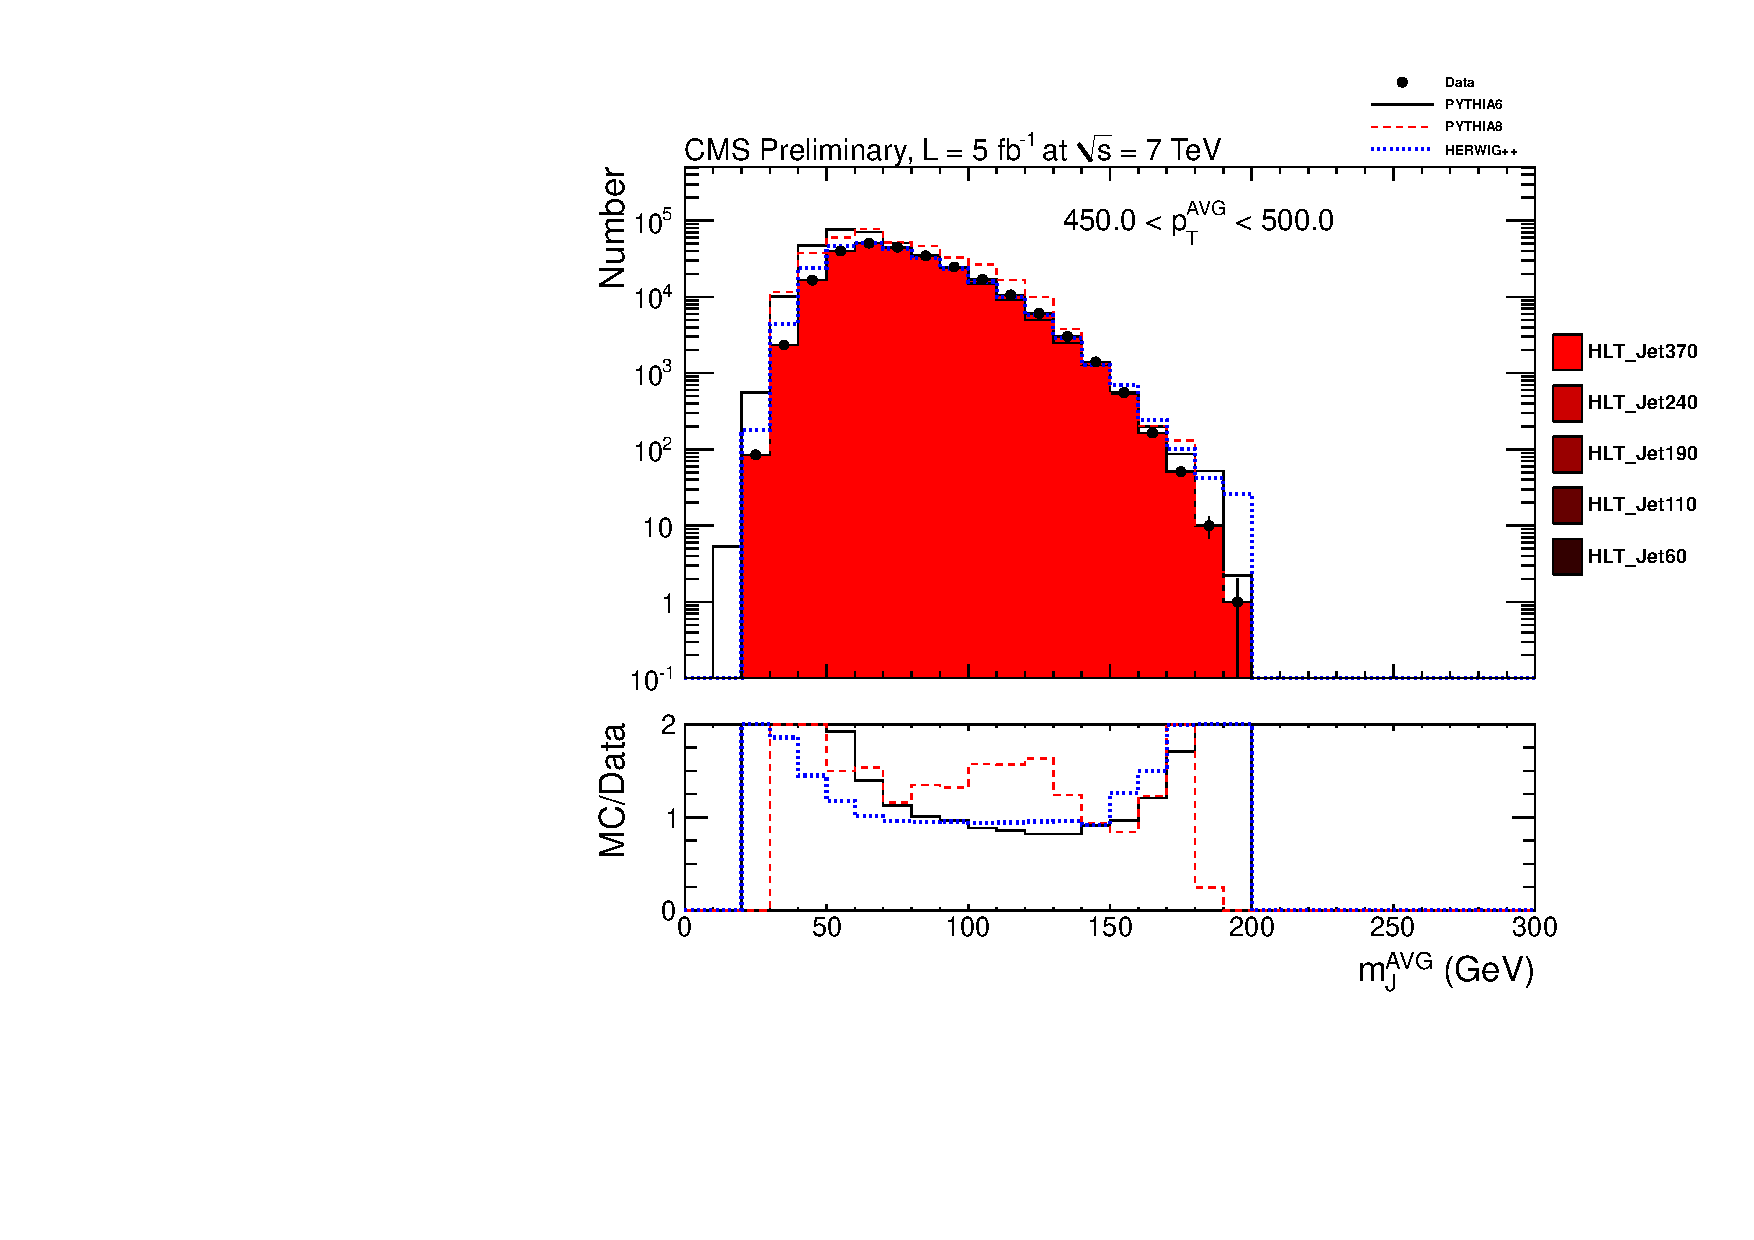
\includegraphics[width=0.95\textwidth]{figs/histAK7MjetVsPtAvg_rawDataMCComparisons_stacktrigs_pt_6}
\caption{Detector-level distributions of the jet mass for AK7 jets,
for $450.0 < \pt^{AVG} < 500.0$ \GeVc. The data are shown in black points.
The simulated distribution from \PYTHIA is shown in solid black, 
the from \PYTHIAEIGHT in dashed red, and from \HERWIG in dotted blue. 
The bottom frame shows the ratio of the simulated distribution
to the distribution from data. The various trigger contributions are shown in shades of red.
\label{figs:histAK7MjetVsPtAvg_rawDataMCComparisons_stacktrigs_pt_6}}
\end{figure}



\begin{figure}[htbp]
\centering
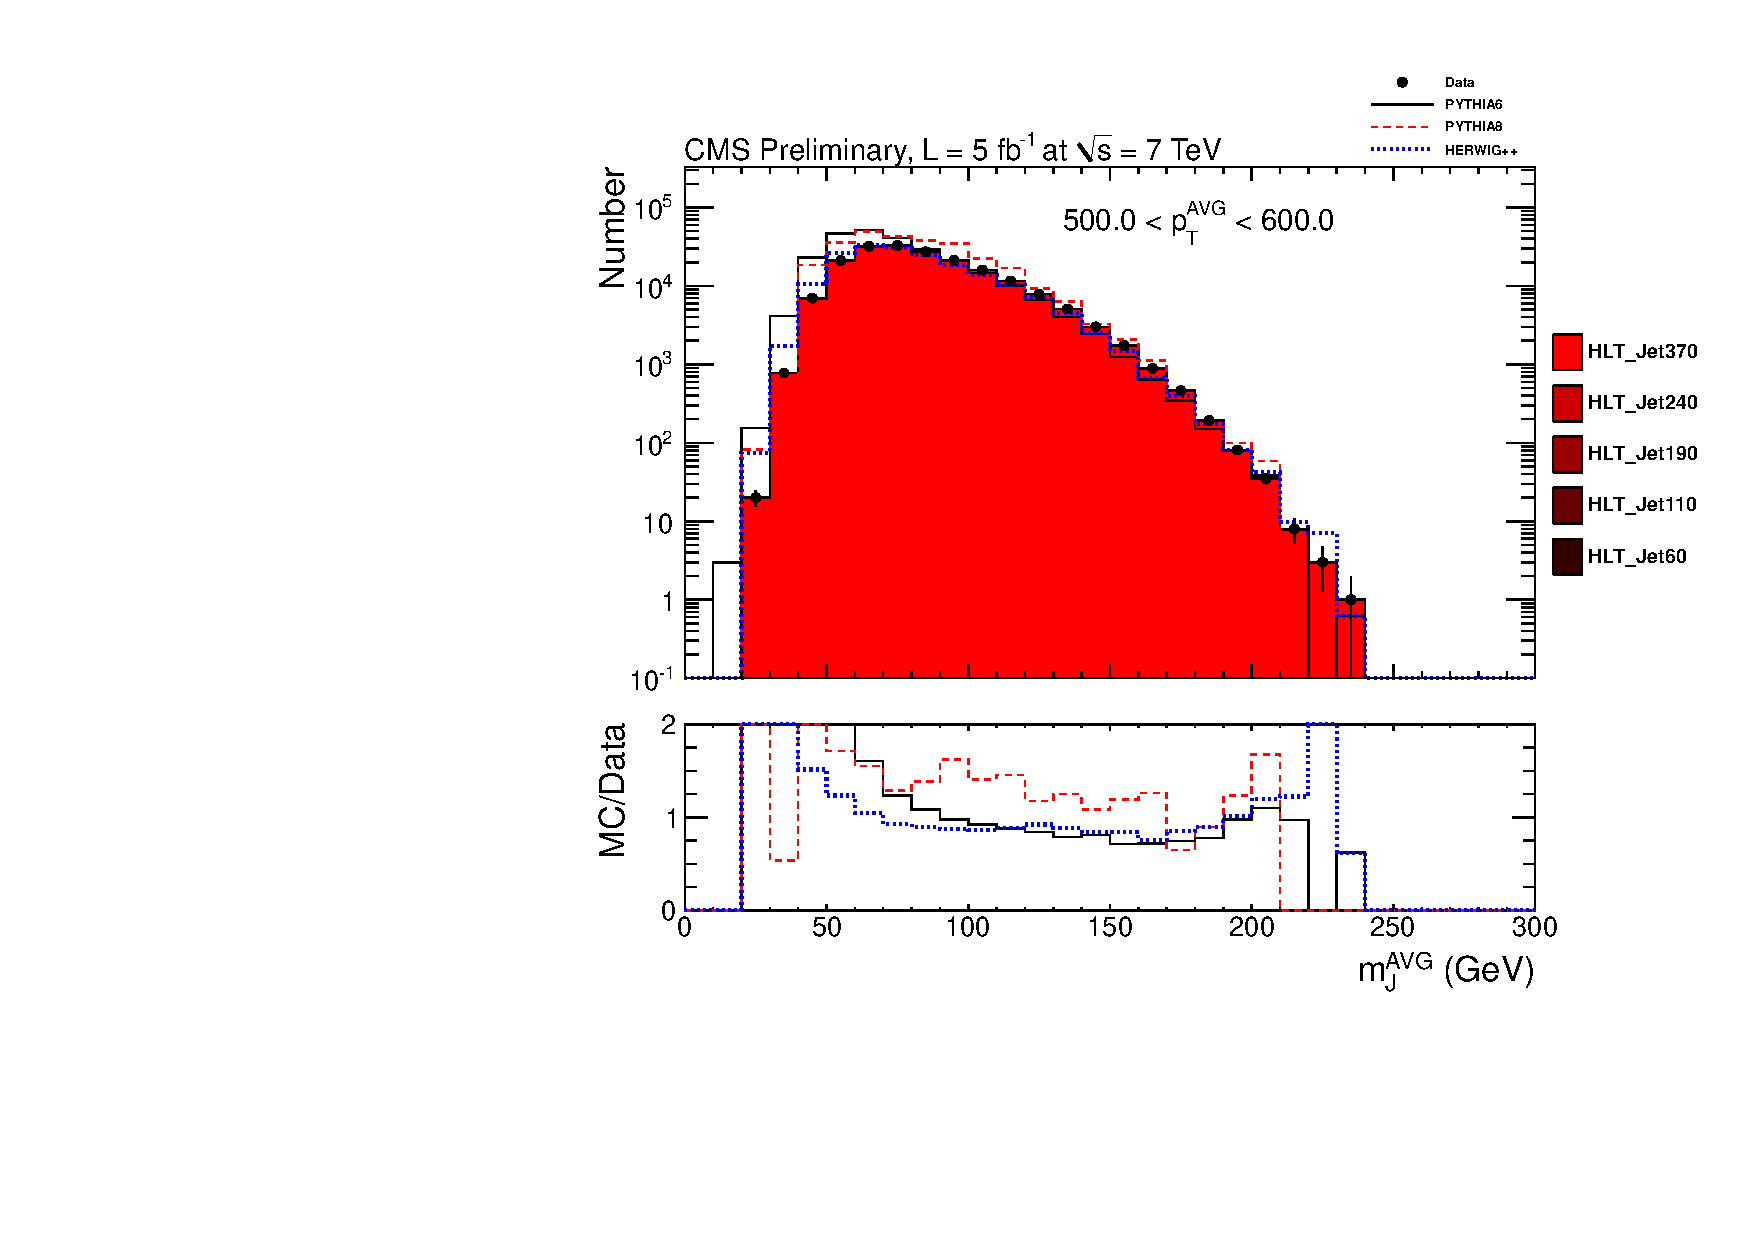
\includegraphics[width=0.95\textwidth]{figs/histAK7MjetVsPtAvg_rawDataMCComparisons_stacktrigs_pt_7}
\caption{Detector-level distributions of the jet mass for AK7 jets,
for $500.0 < \pt^{AVG} < 600.0$ \GeVc. The data are shown in black points.
The simulated distribution from \PYTHIA is shown in solid black, 
the from \PYTHIAEIGHT in dashed red, and from \HERWIG in dotted blue. 
The bottom frame shows the ratio of the simulated distribution
to the distribution from data. The various trigger contributions are shown in shades of red.
\label{figs:histAK7MjetVsPtAvg_rawDataMCComparisons_stacktrigs_pt_7}}
\end{figure}



\begin{figure}[htbp]
\centering
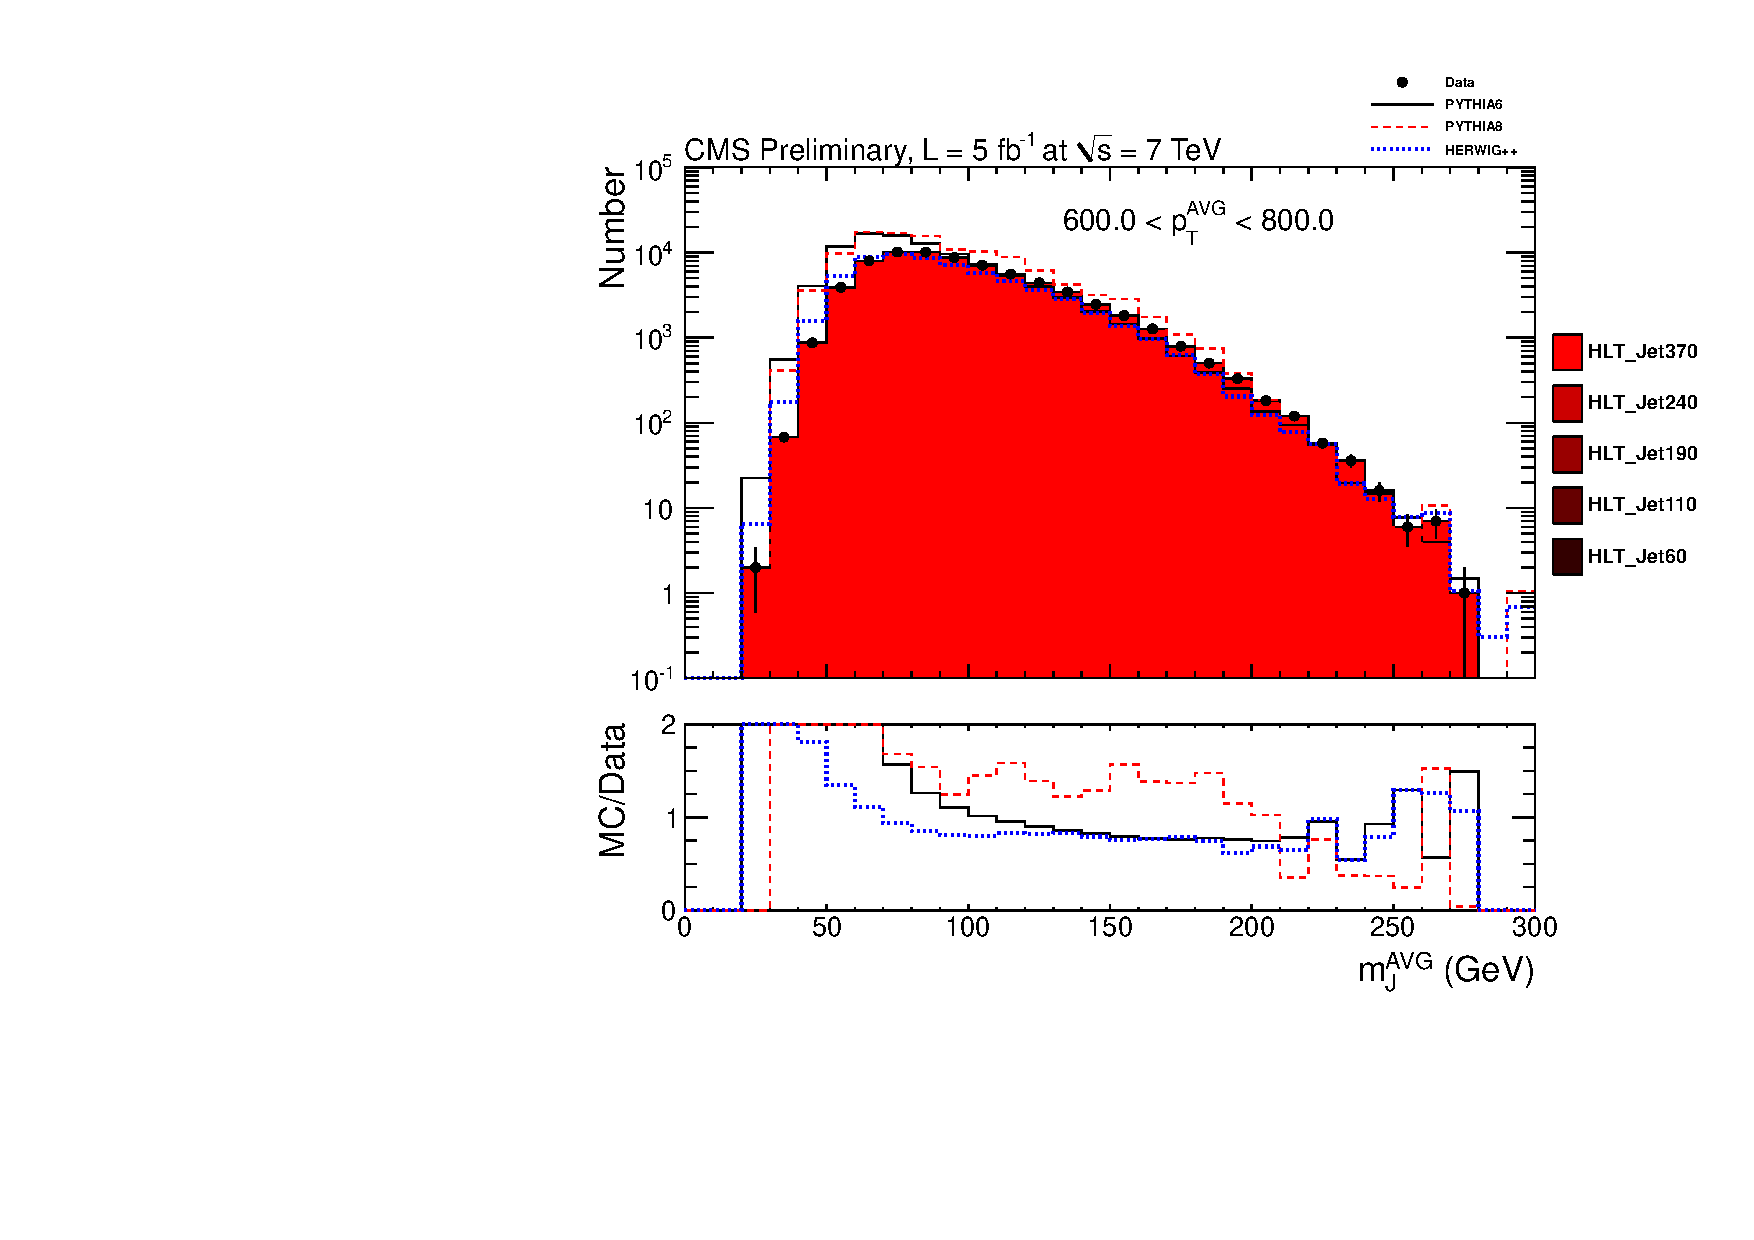
\includegraphics[width=0.95\textwidth]{figs/histAK7MjetVsPtAvg_rawDataMCComparisons_stacktrigs_pt_8}
\caption{Detector-level distributions of the jet mass for AK7 jets,
for $600.0 < \pt^{AVG} < 800.0$ \GeVc. The data are shown in black points.
The simulated distribution from \PYTHIA is shown in solid black, 
the from \PYTHIAEIGHT in dashed red, and from \HERWIG in dotted blue. 
The bottom frame shows the ratio of the simulated distribution
to the distribution from data. The various trigger contributions are shown in shades of red.
\label{figs:histAK7MjetVsPtAvg_rawDataMCComparisons_stacktrigs_pt_8}}
\end{figure}



\begin{figure}[htbp]
\centering
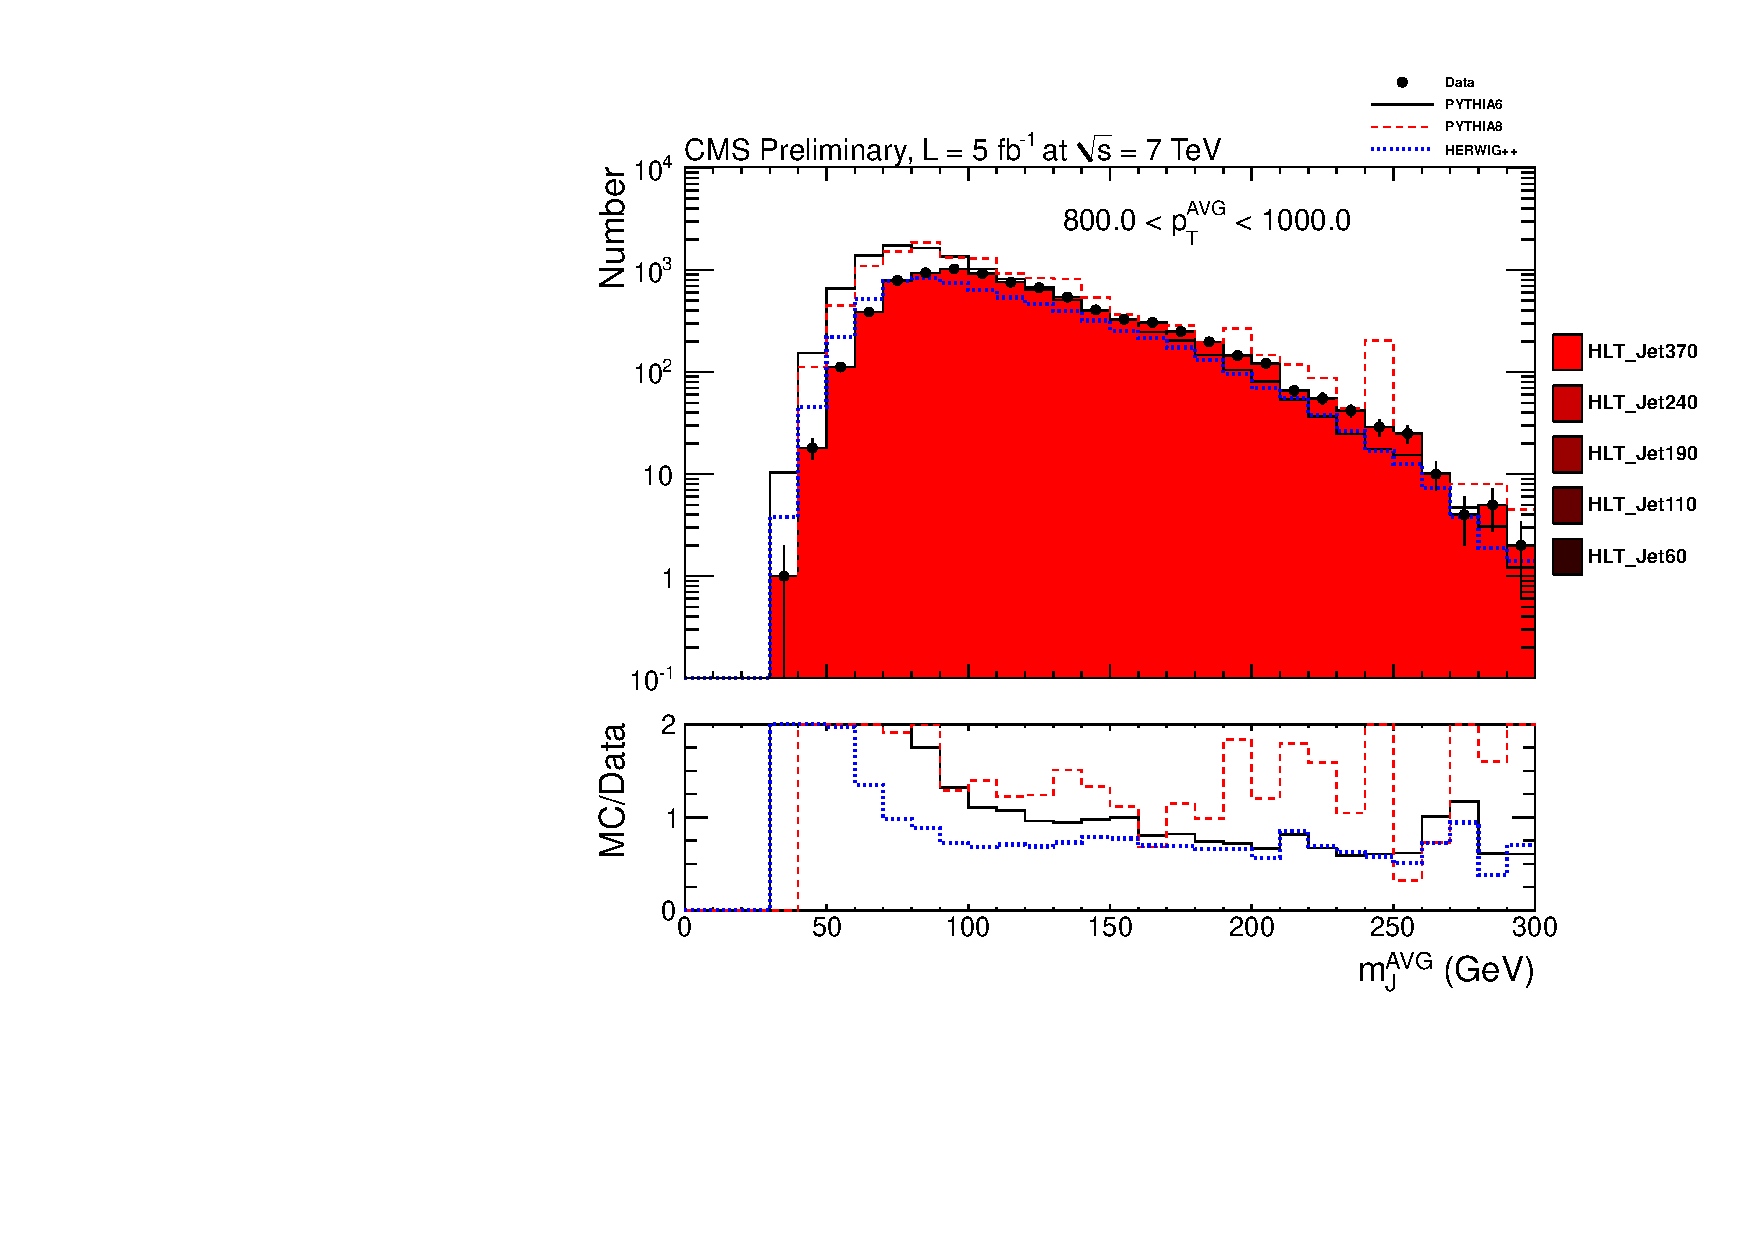
\includegraphics[width=0.95\textwidth]{figs/histAK7MjetVsPtAvg_rawDataMCComparisons_stacktrigs_pt_9}
\caption{Detector-level distributions of the jet mass for AK7 jets,
for $800.0 < \pt^{AVG} < 1000.0$ \GeVc. The data are shown in black points.
The simulated distribution from \PYTHIA is shown in solid black, 
the from \PYTHIAEIGHT in dashed red, and from \HERWIG in dotted blue. 
The bottom frame shows the ratio of the simulated distribution
to the distribution from data. The various trigger contributions are shown in shades of red.
\label{figs:histAK7MjetVsPtAvg_rawDataMCComparisons_stacktrigs_pt_9}}
\end{figure}



\begin{figure}[htbp]
\centering
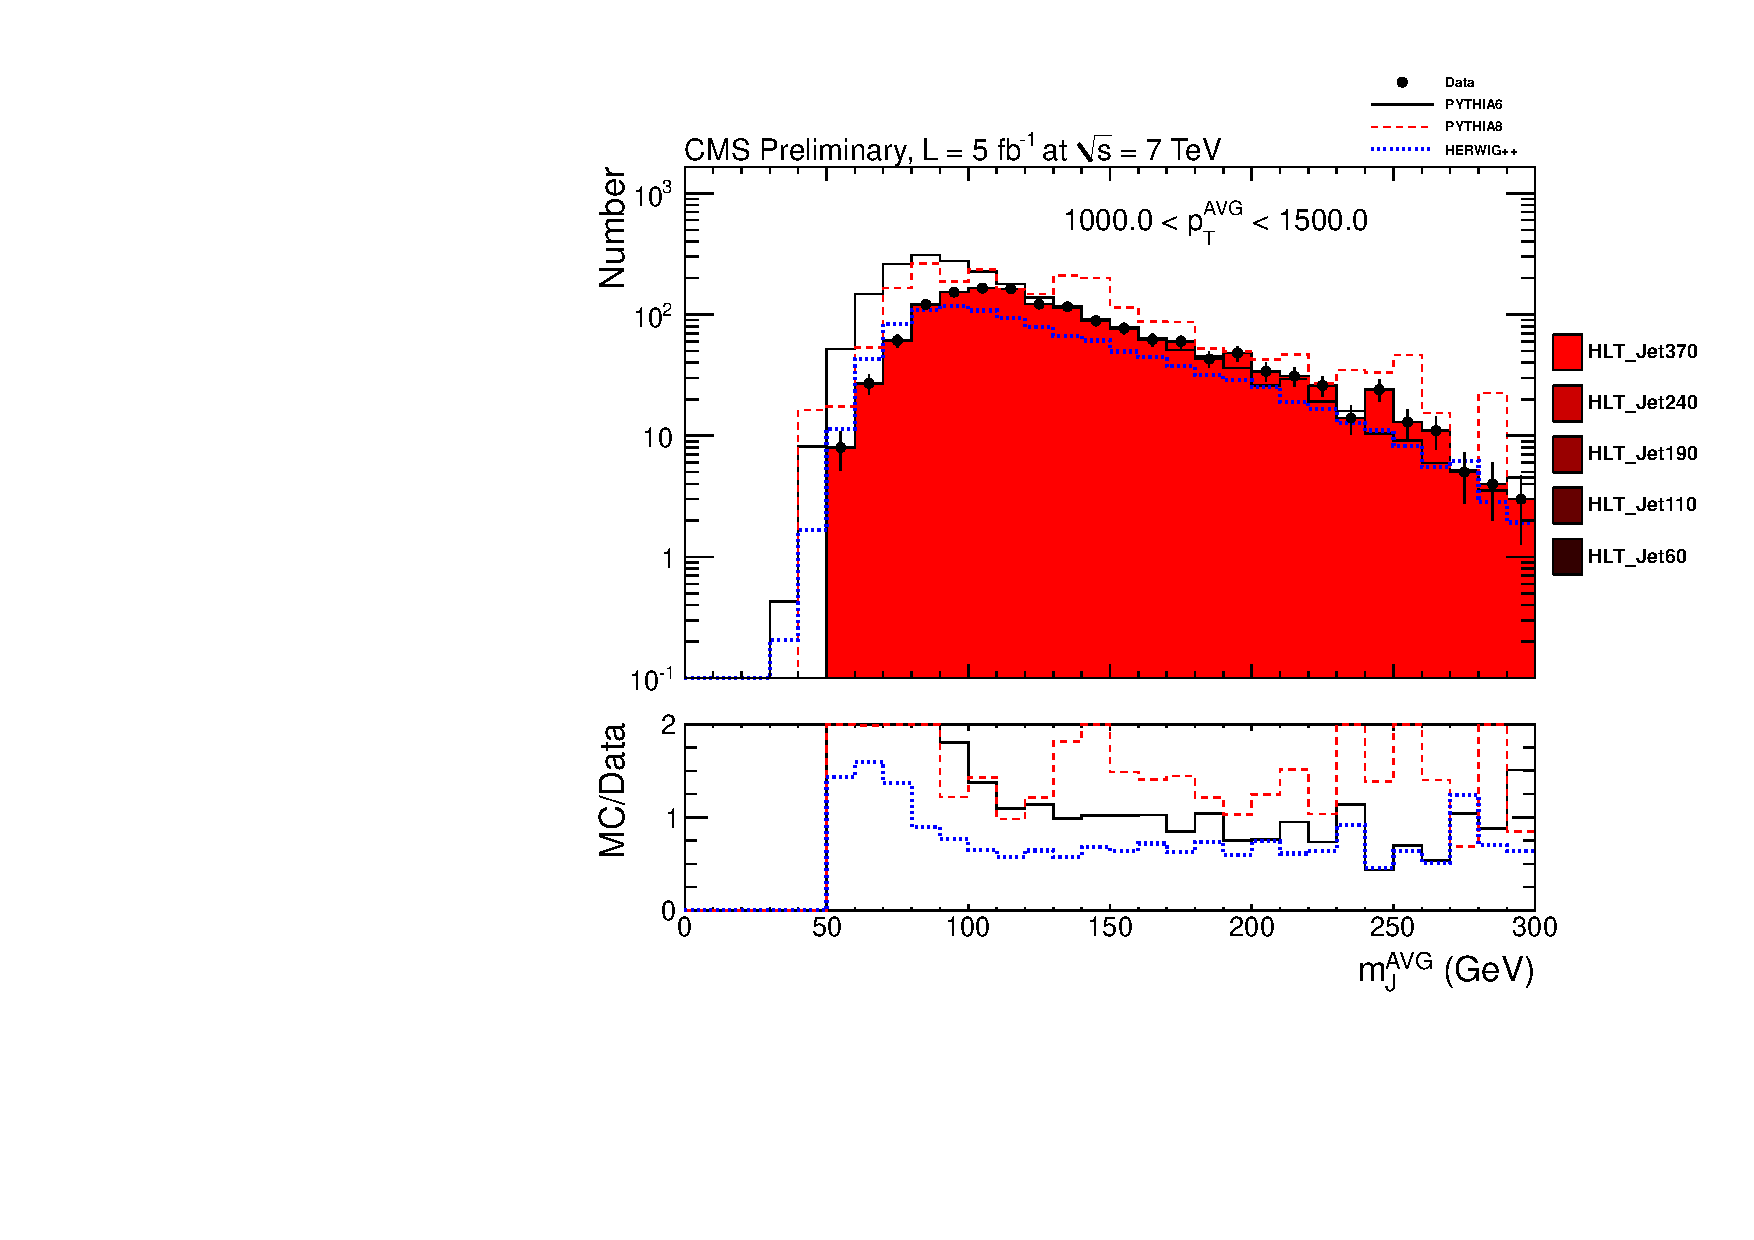
\includegraphics[width=0.95\textwidth]{figs/histAK7MjetVsPtAvg_rawDataMCComparisons_stacktrigs_pt_10}
\caption{Detector-level distributions of the jet mass for AK7 jets,
for $1000.0 < \pt^{AVG} < 1500.0$ \GeVc. The data are shown in black points.
The simulated distribution from \PYTHIA is shown in solid black, 
the from \PYTHIAEIGHT in dashed red, and from \HERWIG in dotted blue. 
The bottom frame shows the ratio of the simulated distribution
to the distribution from data. The various trigger contributions are shown in shades of red.
\label{figs:histAK7MjetVsPtAvg_rawDataMCComparisons_stacktrigs_pt_10}}
\end{figure}

\clearpage


\fi


\ifnpas 

\begin{figure}[htbp]
\centering
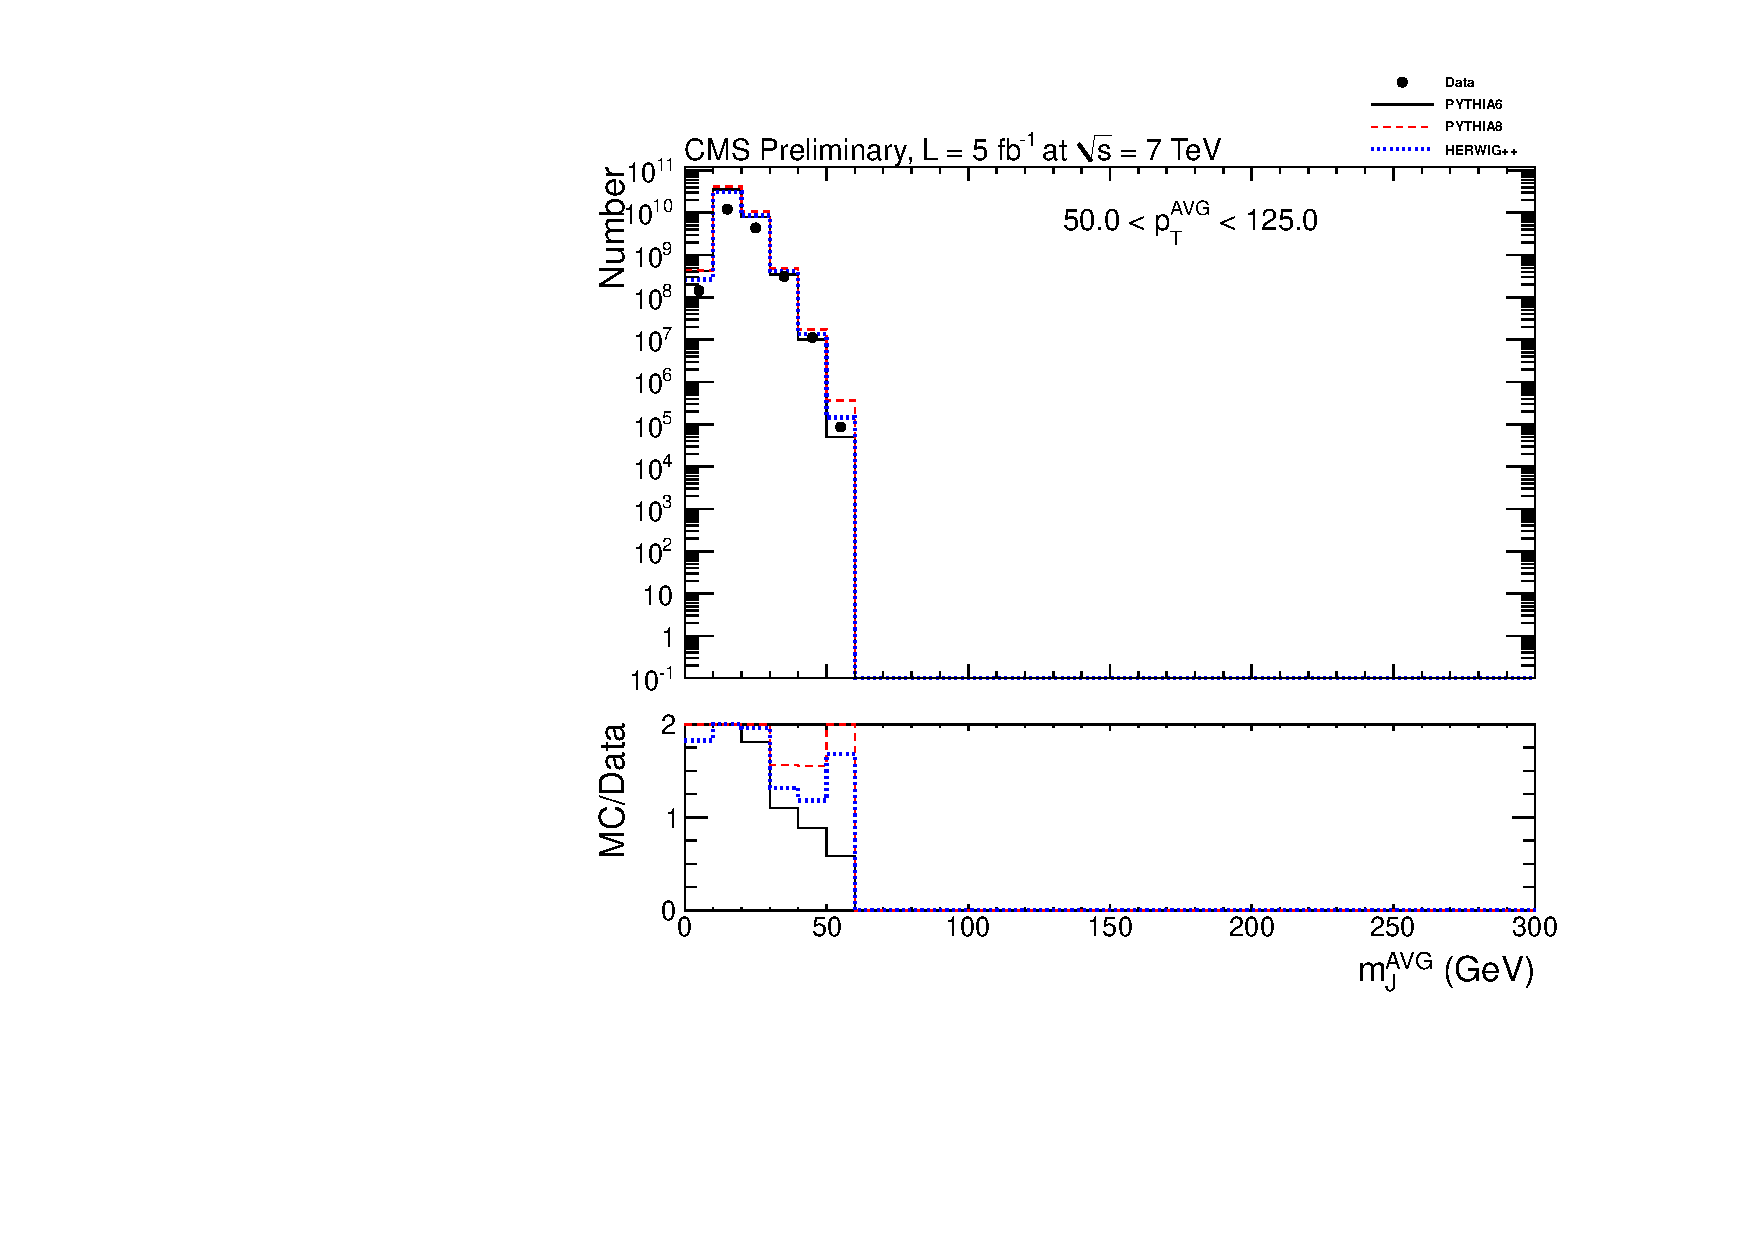
\includegraphics[width=0.95\textwidth]{figs/histAK7MjetVsPtAvg_rawDataMCComparisons_pt_1}
\caption{Detector-level distributions of the jet mass for AK7 jets,
for $50.0 < \pt^{AVG} < 125.0$ \GeVc. The data are shown in black points.
The simulated distribution from \PYTHIA is shown in solid black, 
the from \PYTHIAEIGHT in dashed red, and from \HERWIG in dotted blue. 
The bottom frame shows the ratio of the simulated distribution
to the distribution from data. 
\label{figs:histAK7MjetVsPtAvg_rawDataMCComparisons_pt_1}}
\end{figure}
\fi


\begin{figure}[htbp]
\centering
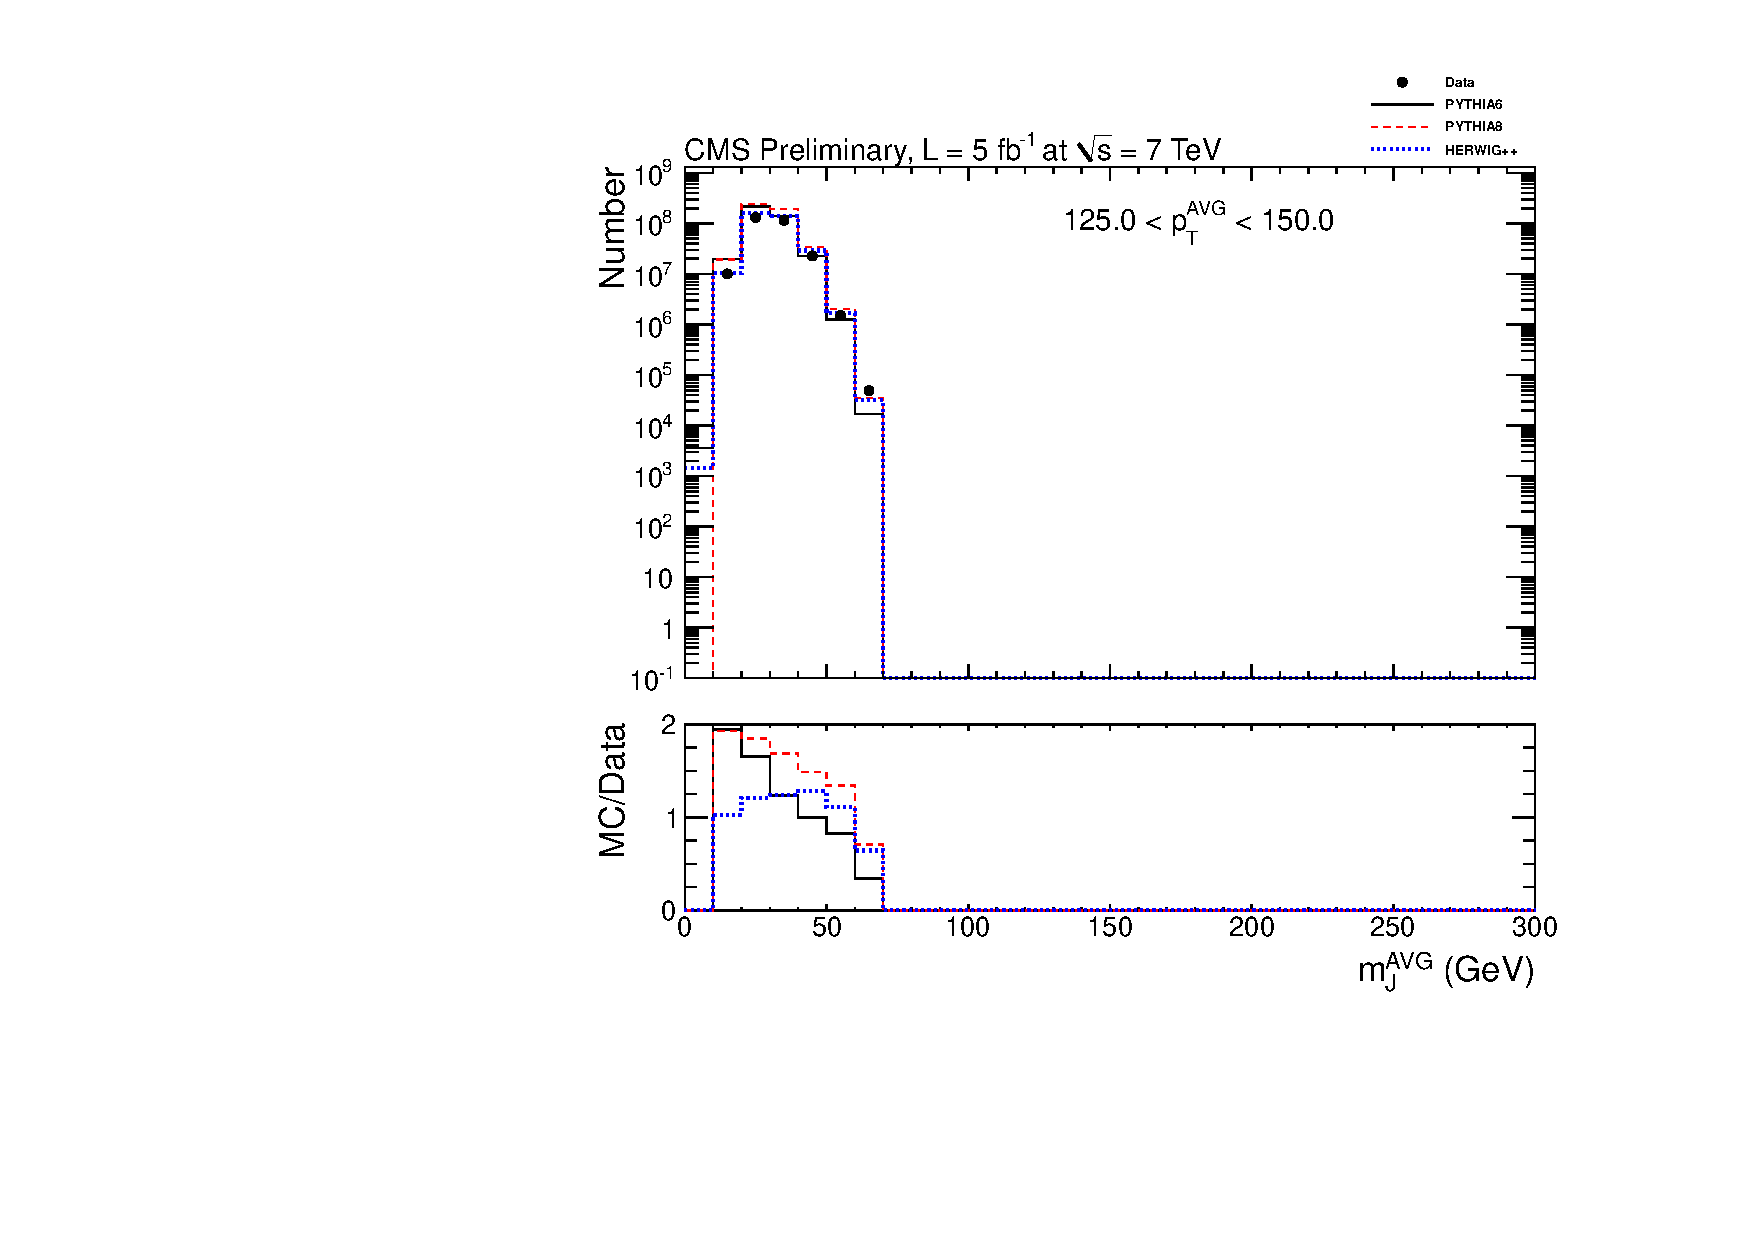
\includegraphics[width=0.49\textwidth]{figs/histAK7MjetVsPtAvg_rawDataMCComparisons_pt_2}
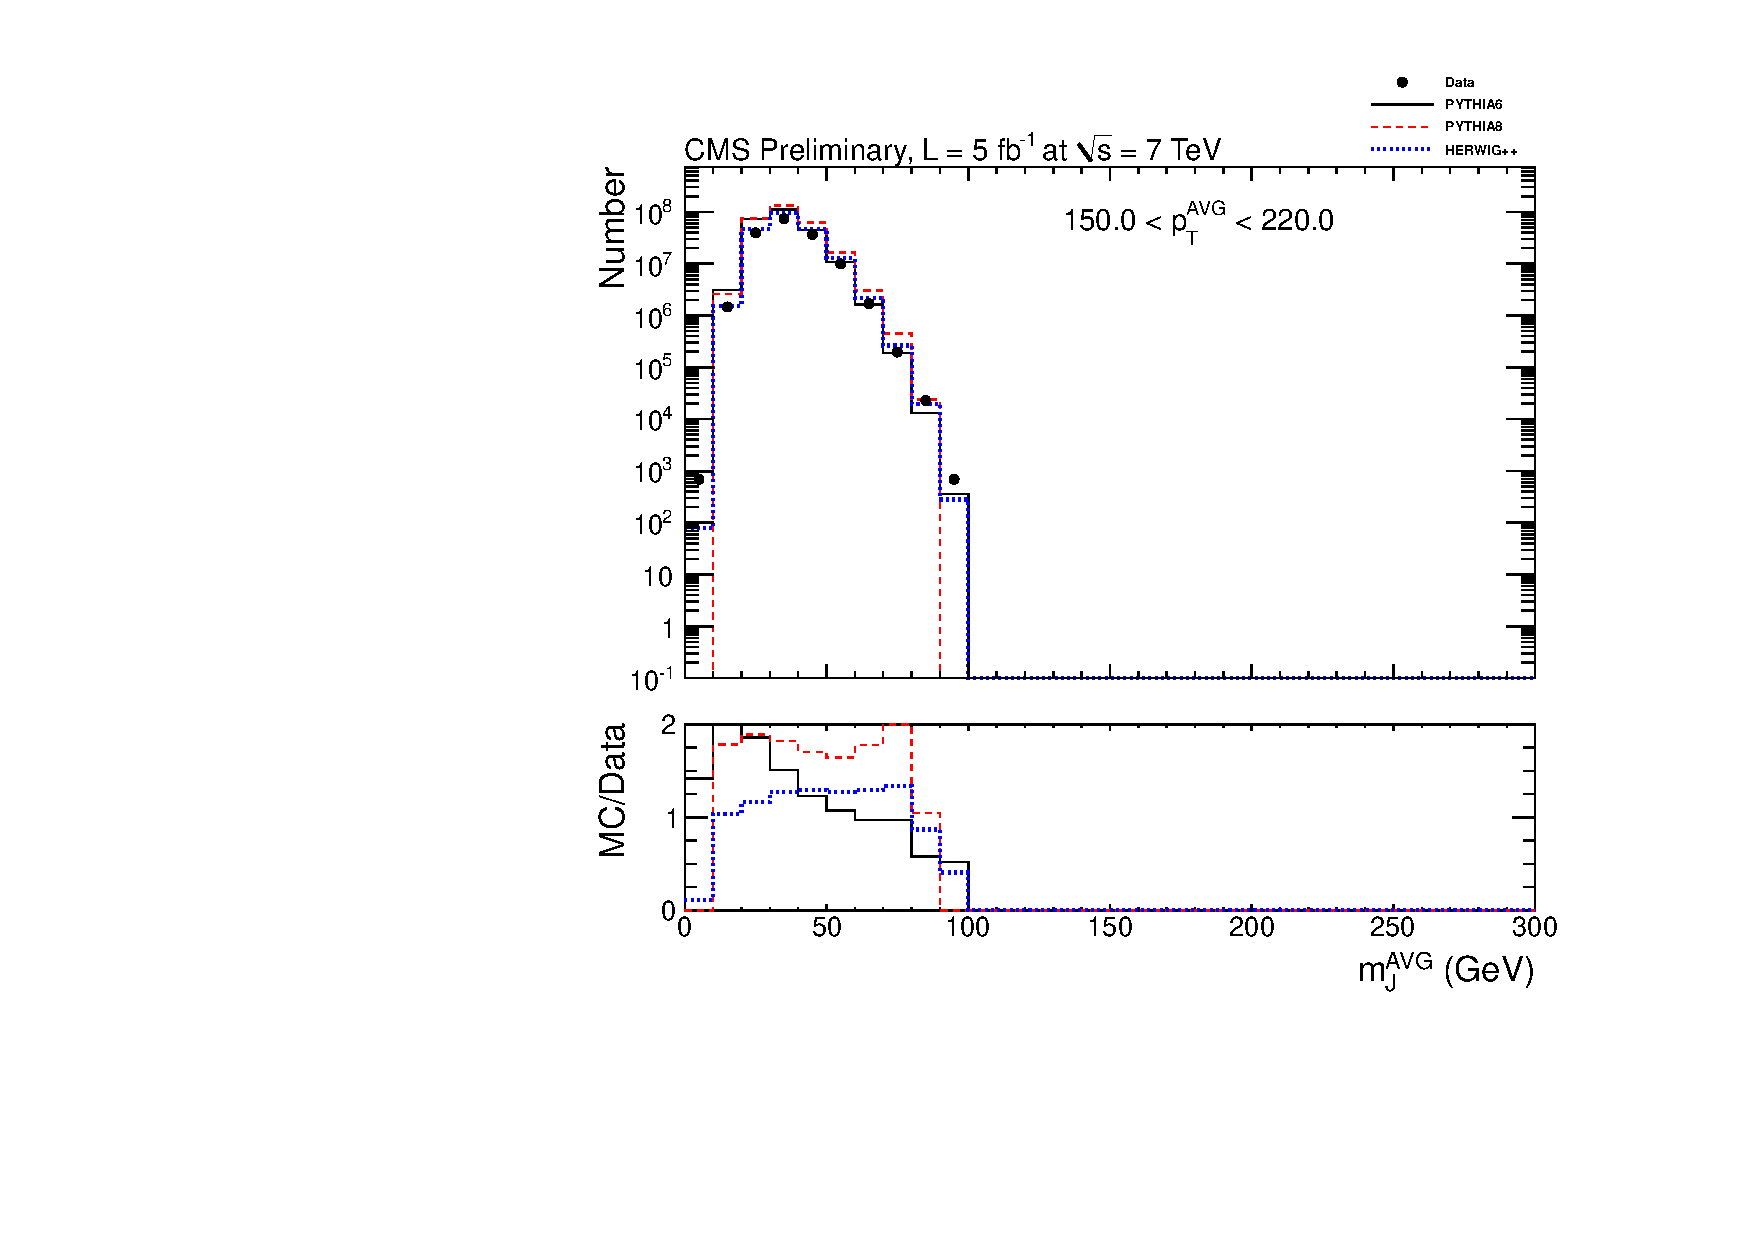
\includegraphics[width=0.49\textwidth]{figs/histAK7MjetVsPtAvg_rawDataMCComparisons_pt_3}
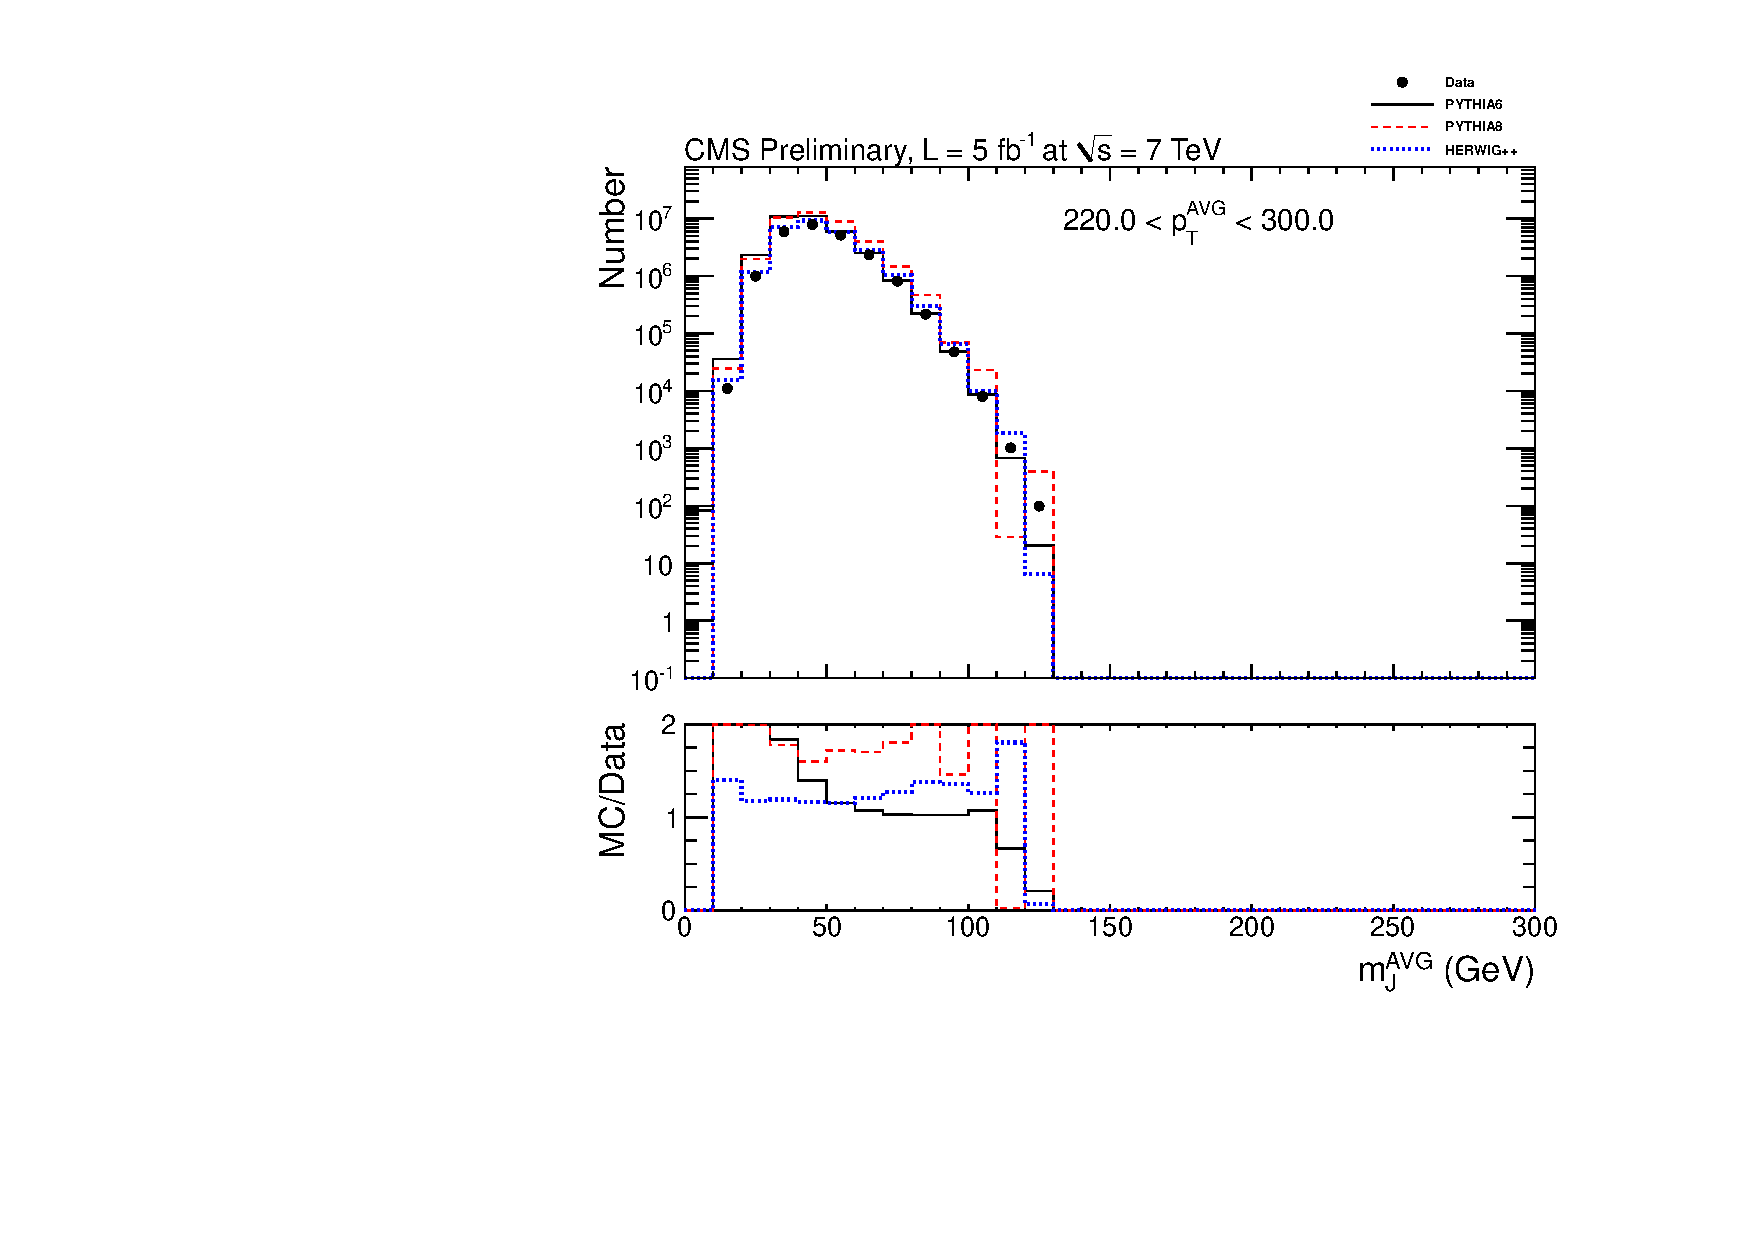
\includegraphics[width=0.49\textwidth]{figs/histAK7MjetVsPtAvg_rawDataMCComparisons_pt_4}
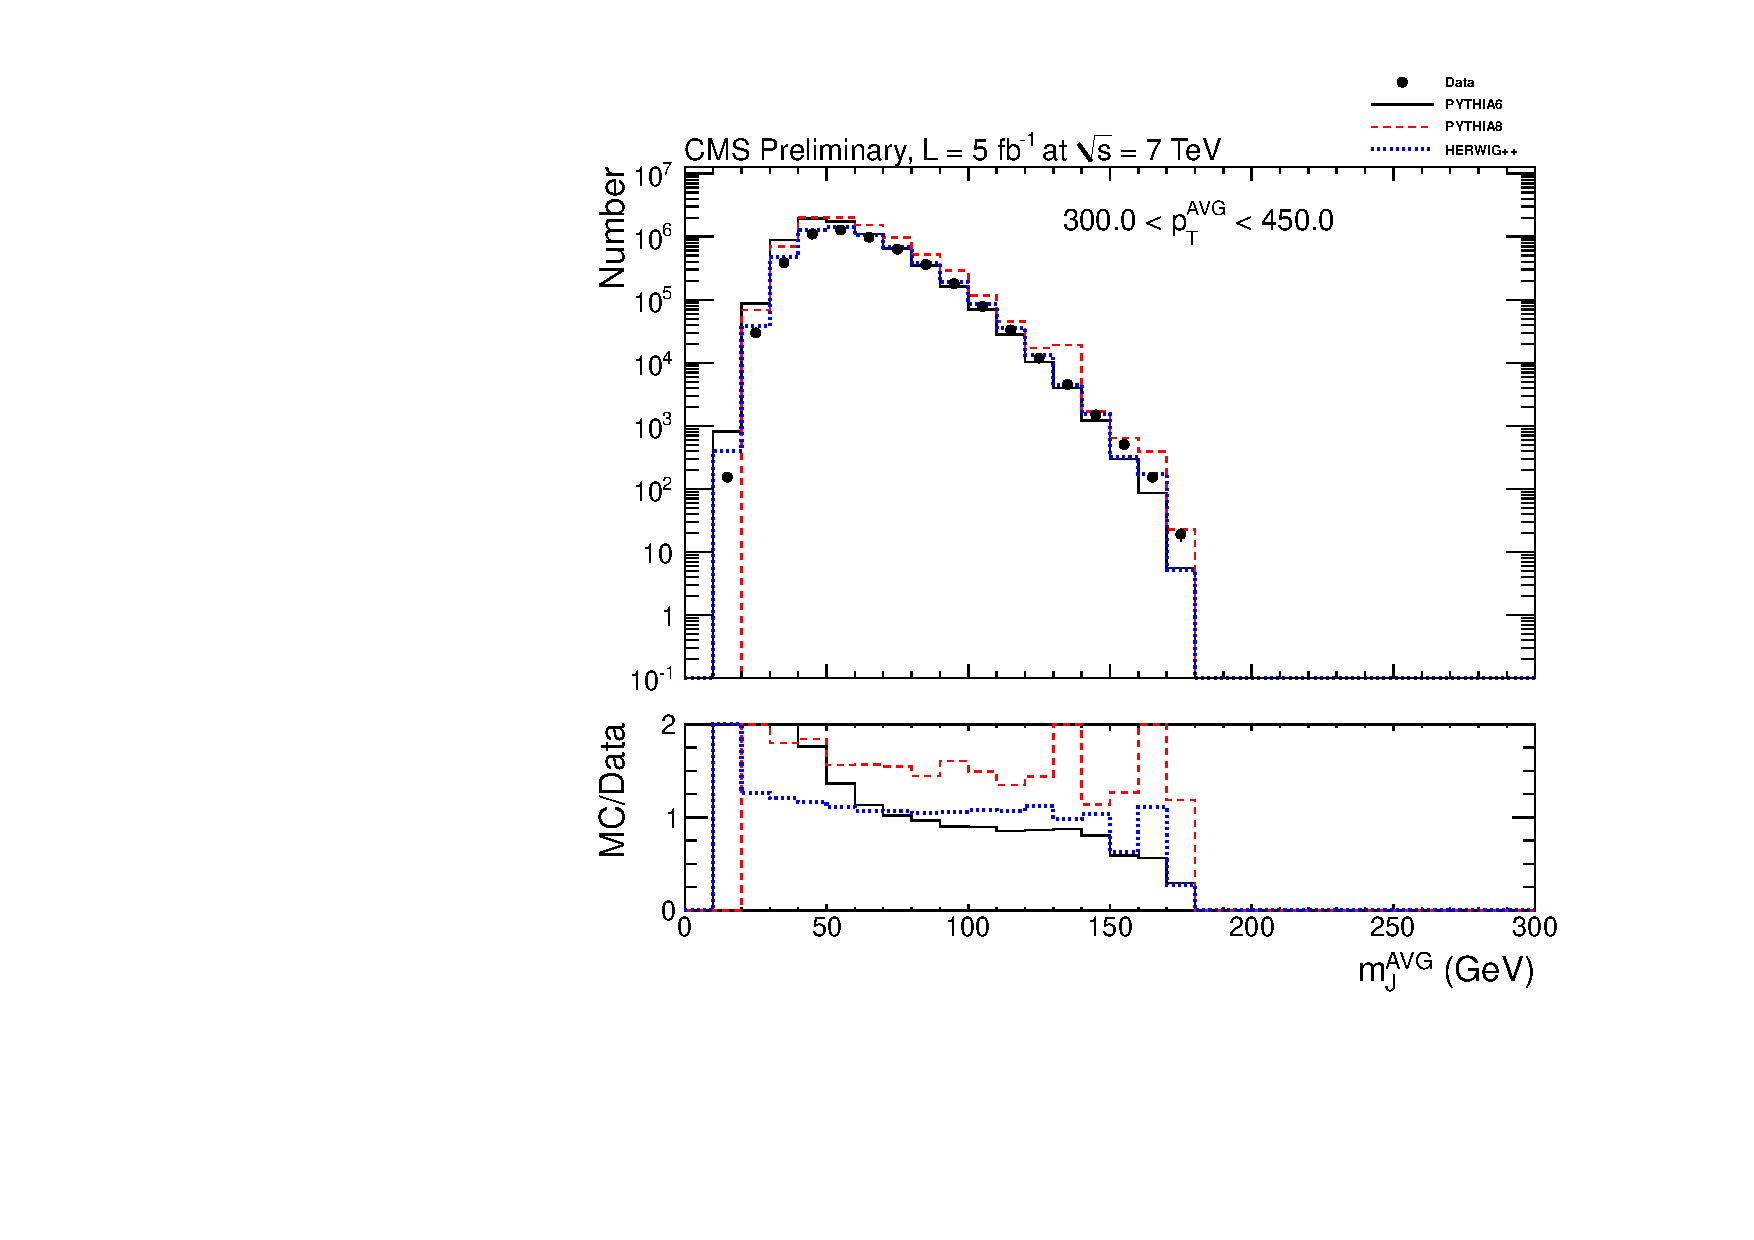
\includegraphics[width=0.49\textwidth]{figs/histAK7MjetVsPtAvg_rawDataMCComparisons_pt_5}
\caption{Detector-level distributions of the jet mass for AK7 jets,
for several $\pt^{AVG}$ bins. The data are shown in black points.
%for $125.0 < \pt^{AVG} < 150.0$ \GeVc. The data are shown in black points.
The simulated distribution from \PYTHIA is shown in solid black, 
the from \PYTHIAEIGHT in dashed red, and from \HERWIG in dotted blue. 
The bottom frame shows the ratio of the simulated distribution
to the distribution from data. 
\label{figs:histAK7MjetVsPtAvg_rawDataMCComparisons_pt_2}}
\end{figure}

%%
\ifnpas

\begin{figure}[htbp]
\centering
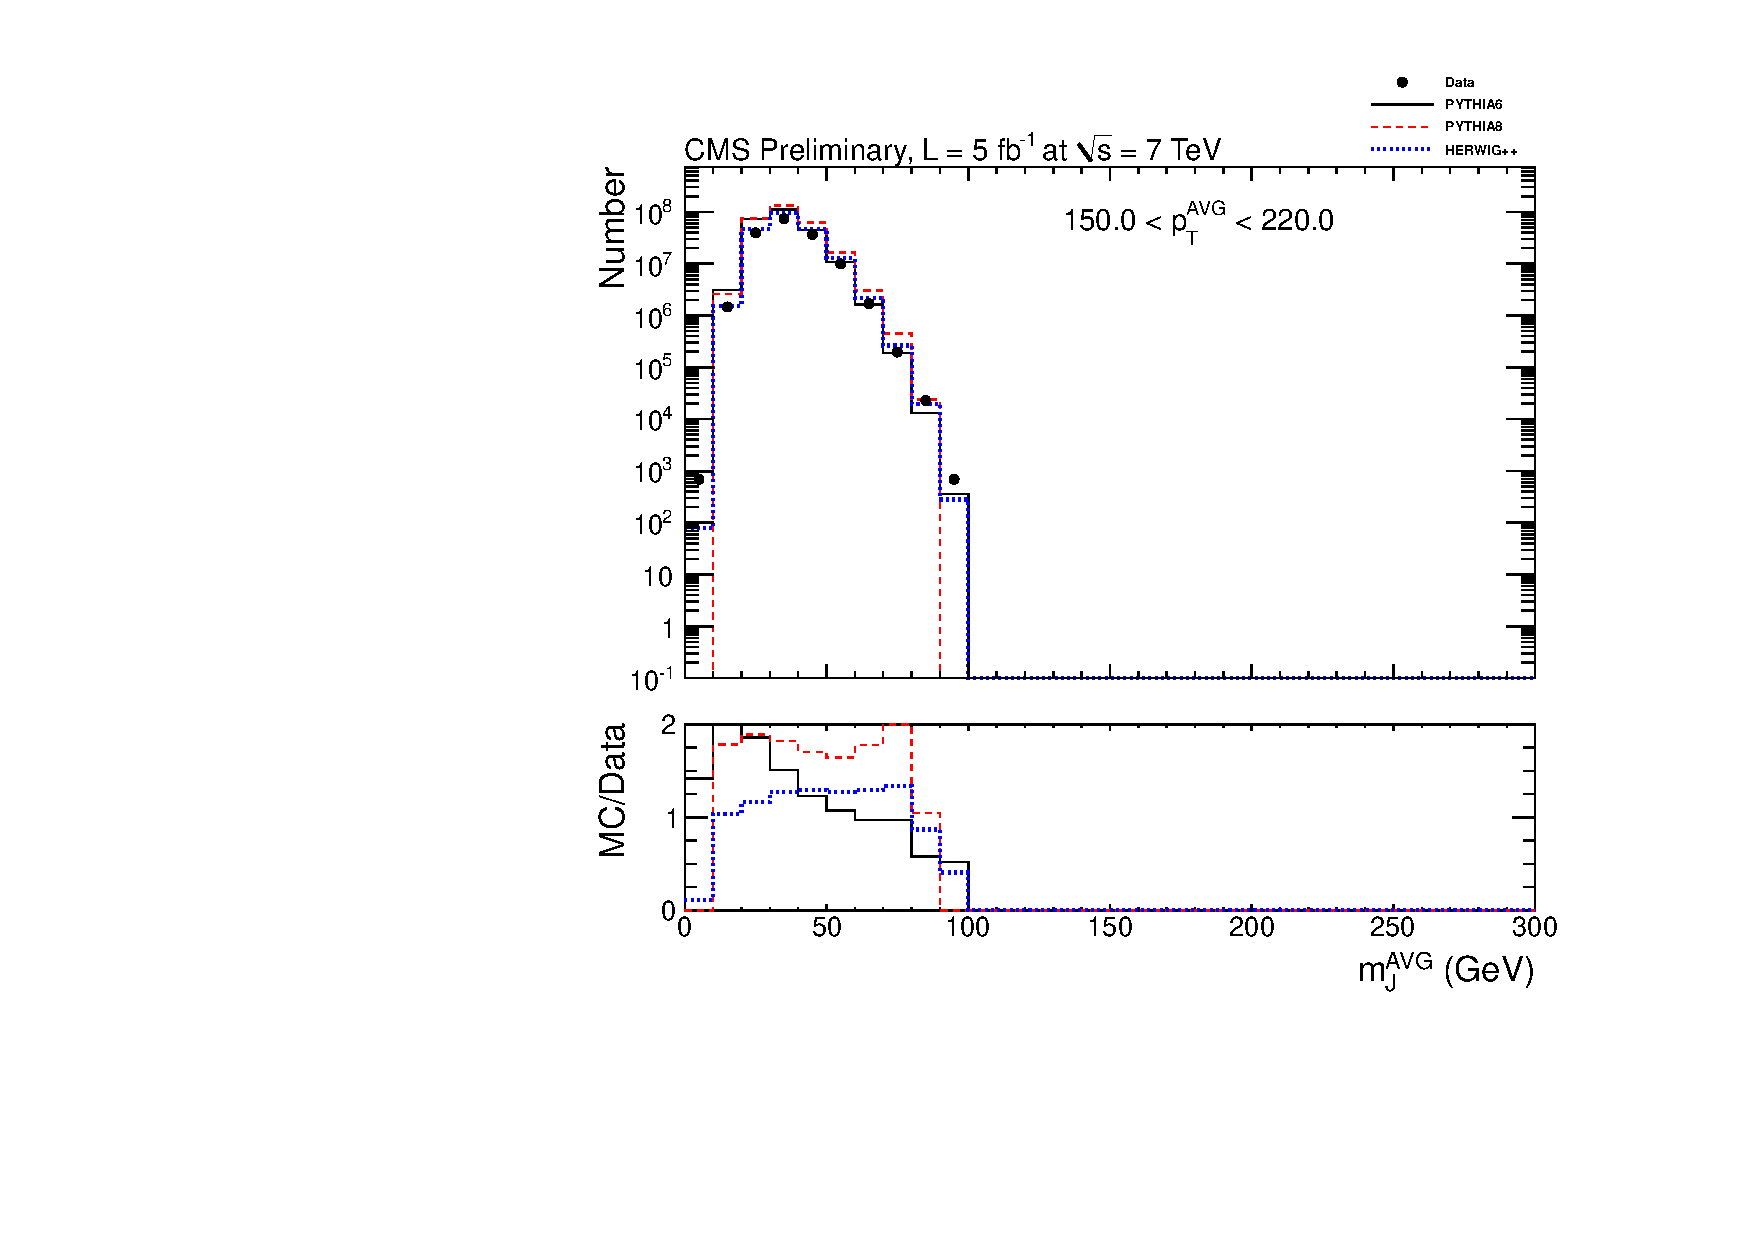
\includegraphics[width=0.95\textwidth]{figs/histAK7MjetVsPtAvg_rawDataMCComparisons_pt_3}
\caption{Detector-level distributions of the jet mass for AK7 jets,
for $150.0 < \pt^{AVG} < 220.0$ \GeVc. The data are shown in black points.
The simulated distribution from \PYTHIA is shown in solid black, 
the from \PYTHIAEIGHT in dashed red, and from \HERWIG in dotted blue. 
The bottom frame shows the ratio of the simulated distribution
to the distribution from data. 
\label{figs:histAK7MjetVsPtAvg_rawDataMCComparisons_pt_3}}
\end{figure}



\begin{figure}[htbp]
\centering
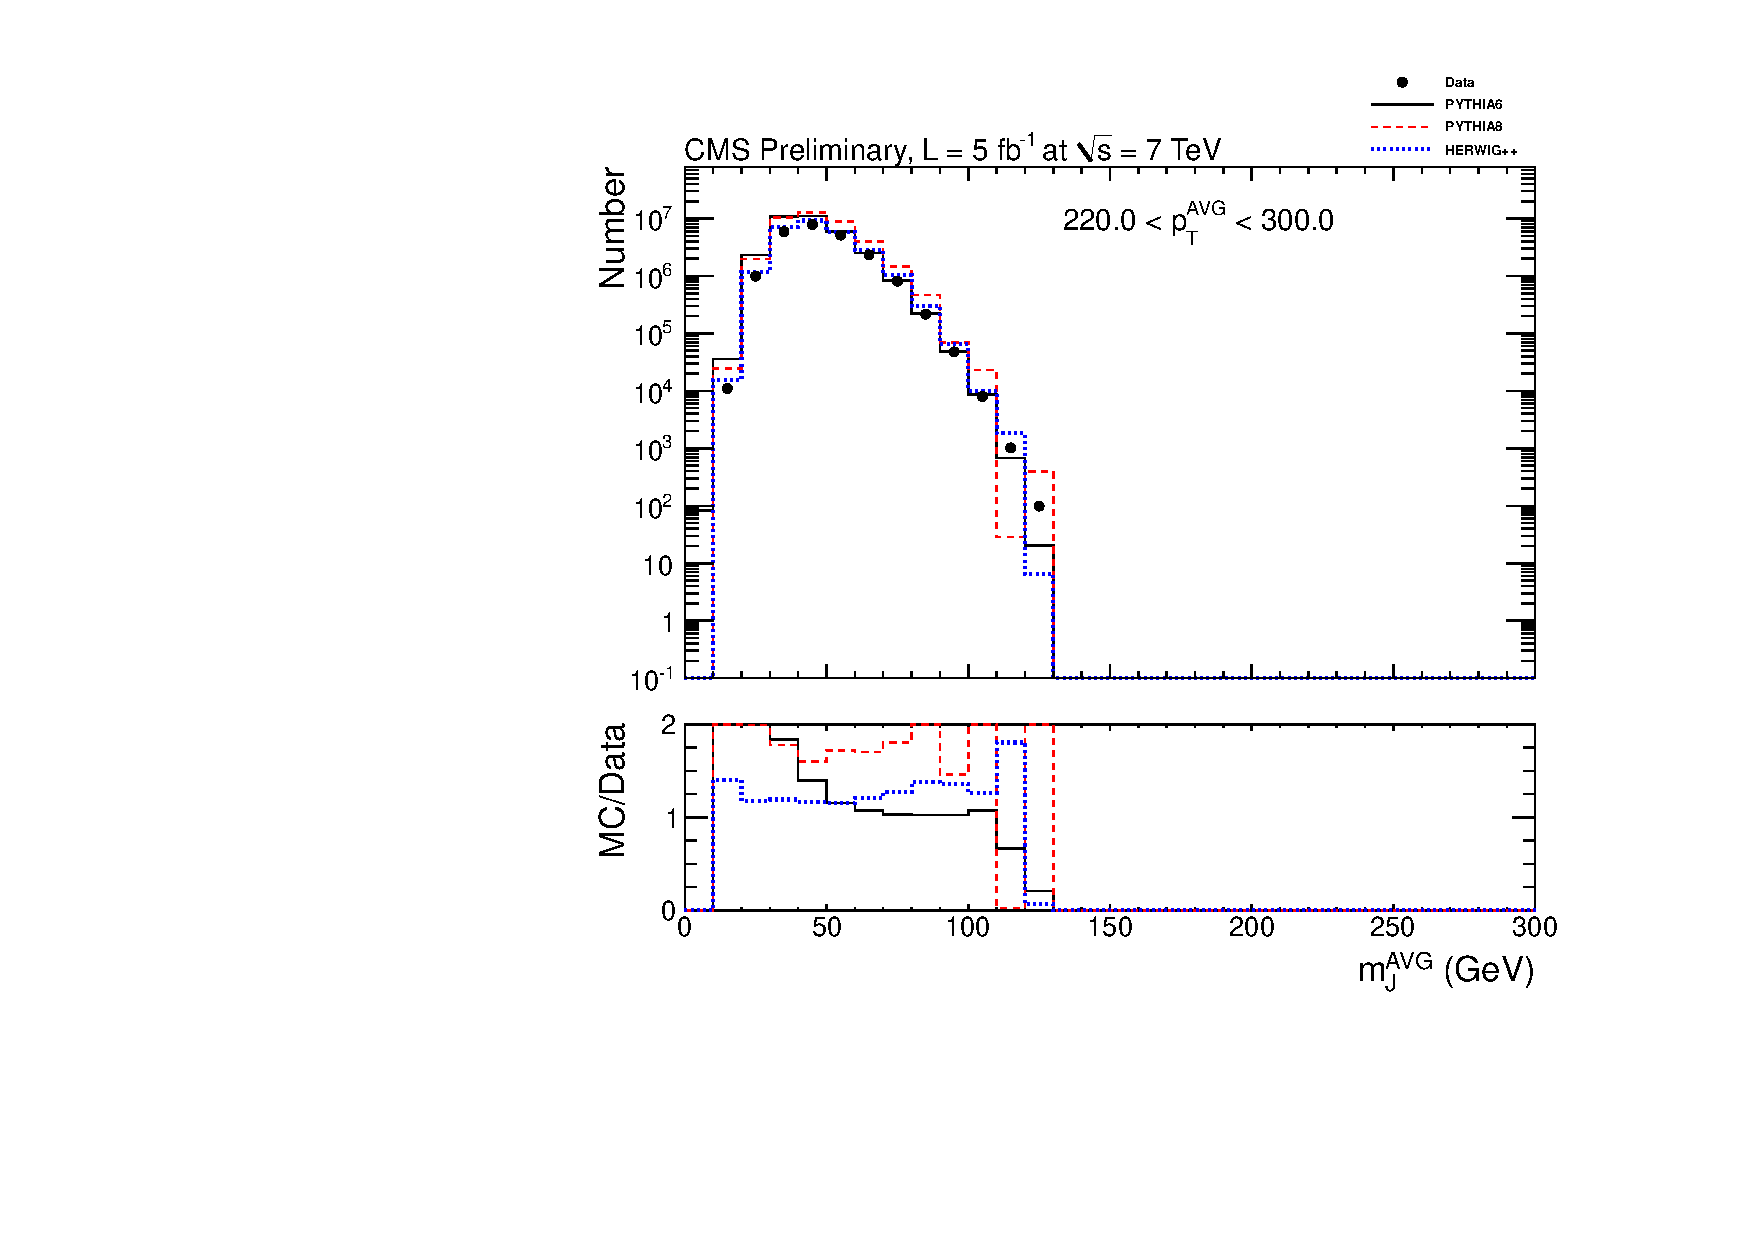
\includegraphics[width=0.95\textwidth]{figs/histAK7MjetVsPtAvg_rawDataMCComparisons_pt_4}
\caption{Detector-level distributions of the jet mass for AK7 jets,
for $220.0 < \pt^{AVG} < 300.0$ \GeVc. The data are shown in black points.
The simulated distribution from \PYTHIA is shown in solid black, 
the from \PYTHIAEIGHT in dashed red, and from \HERWIG in dotted blue. 
The bottom frame shows the ratio of the simulated distribution
to the distribution from data. 
\label{figs:histAK7MjetVsPtAvg_rawDataMCComparisons_pt_4}}
\end{figure}



\begin{figure}[htbp]
\centering
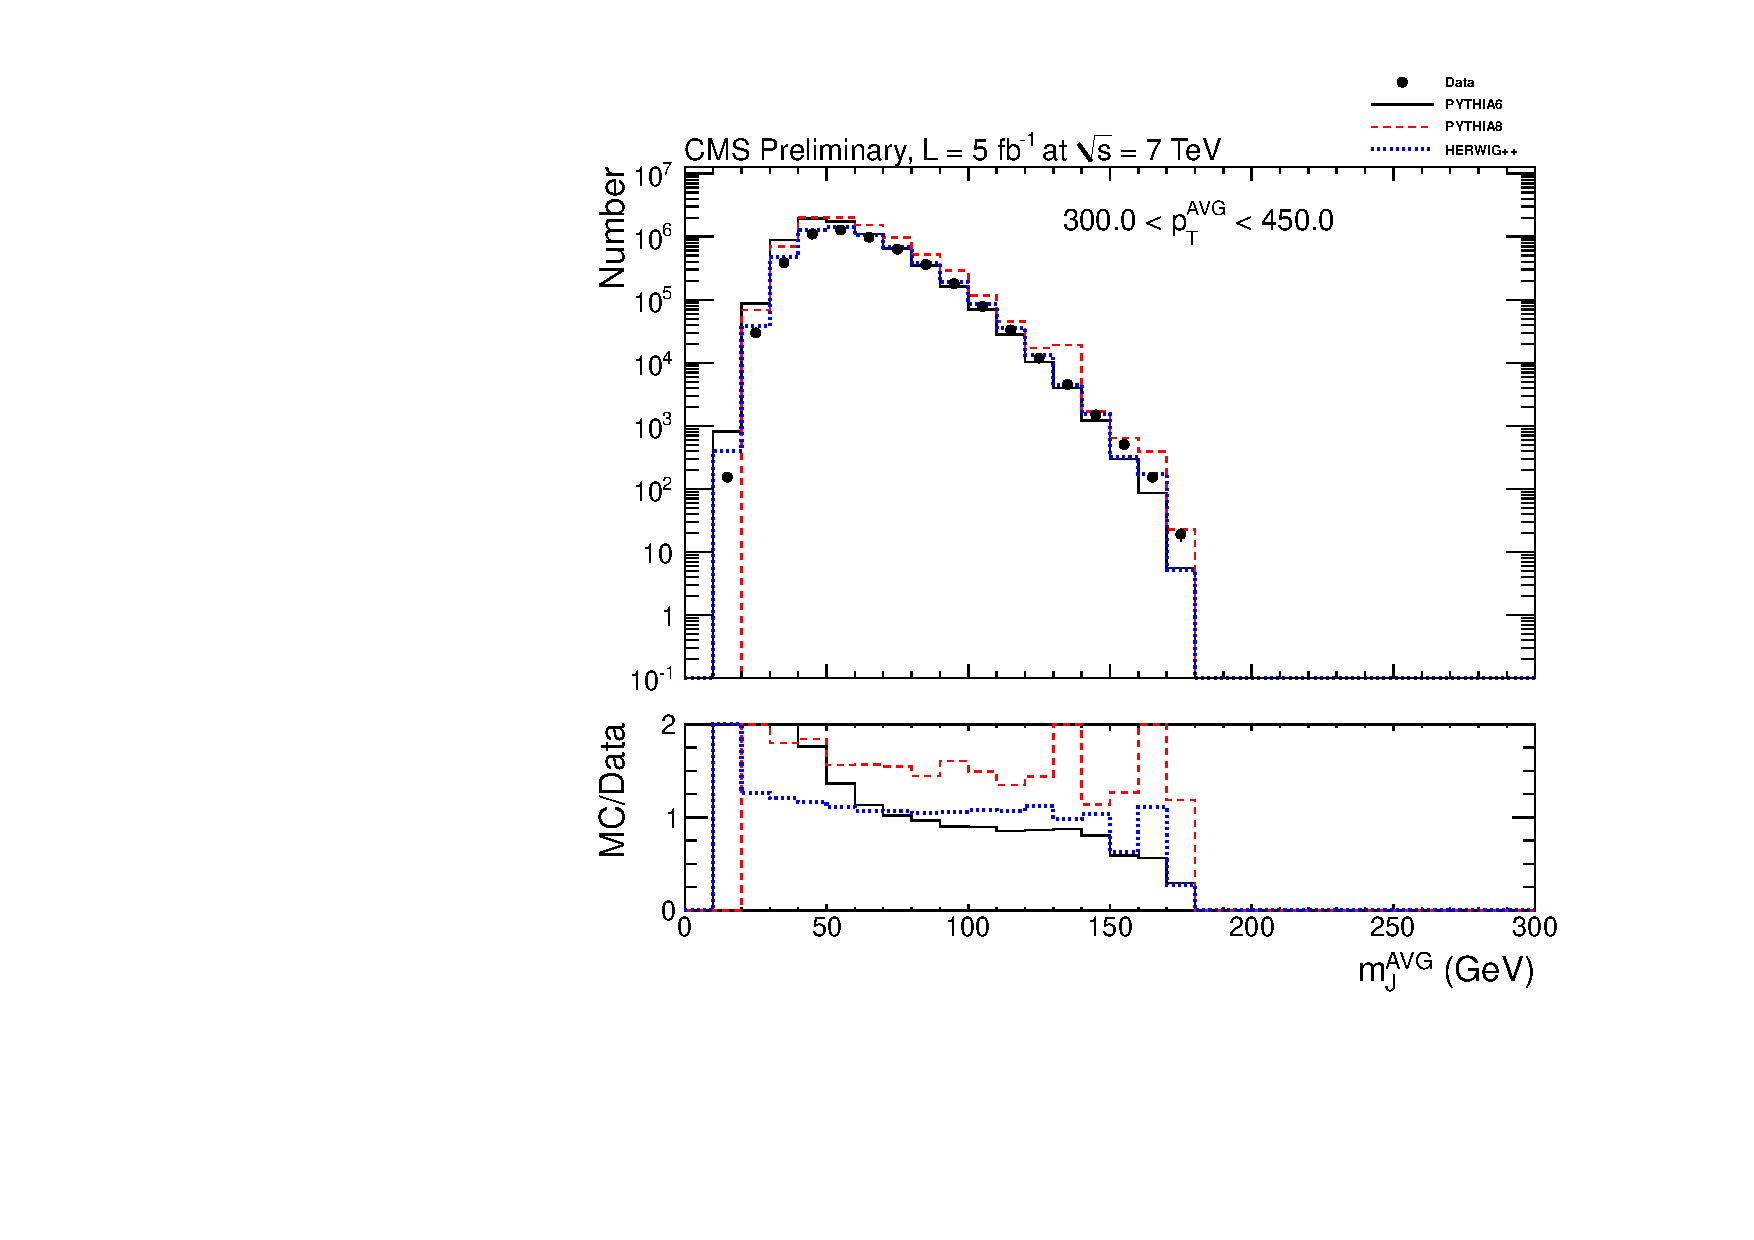
\includegraphics[width=0.95\textwidth]{figs/histAK7MjetVsPtAvg_rawDataMCComparisons_pt_5}
\caption{Detector-level distributions of the jet mass for AK7 jets,
for $300.0 < \pt^{AVG} < 450.0$ \GeVc. The data are shown in black points.
The simulated distribution from \PYTHIA is shown in solid black, 
the from \PYTHIAEIGHT in dashed red, and from \HERWIG in dotted blue. 
The bottom frame shows the ratio of the simulated distribution
to the distribution from data. 
\label{figs:histAK7MjetVsPtAvg_rawDataMCComparisons_pt_5}}
\end{figure}
\fi

%%

\ifnpas

\begin{figure}[htbp]
\centering
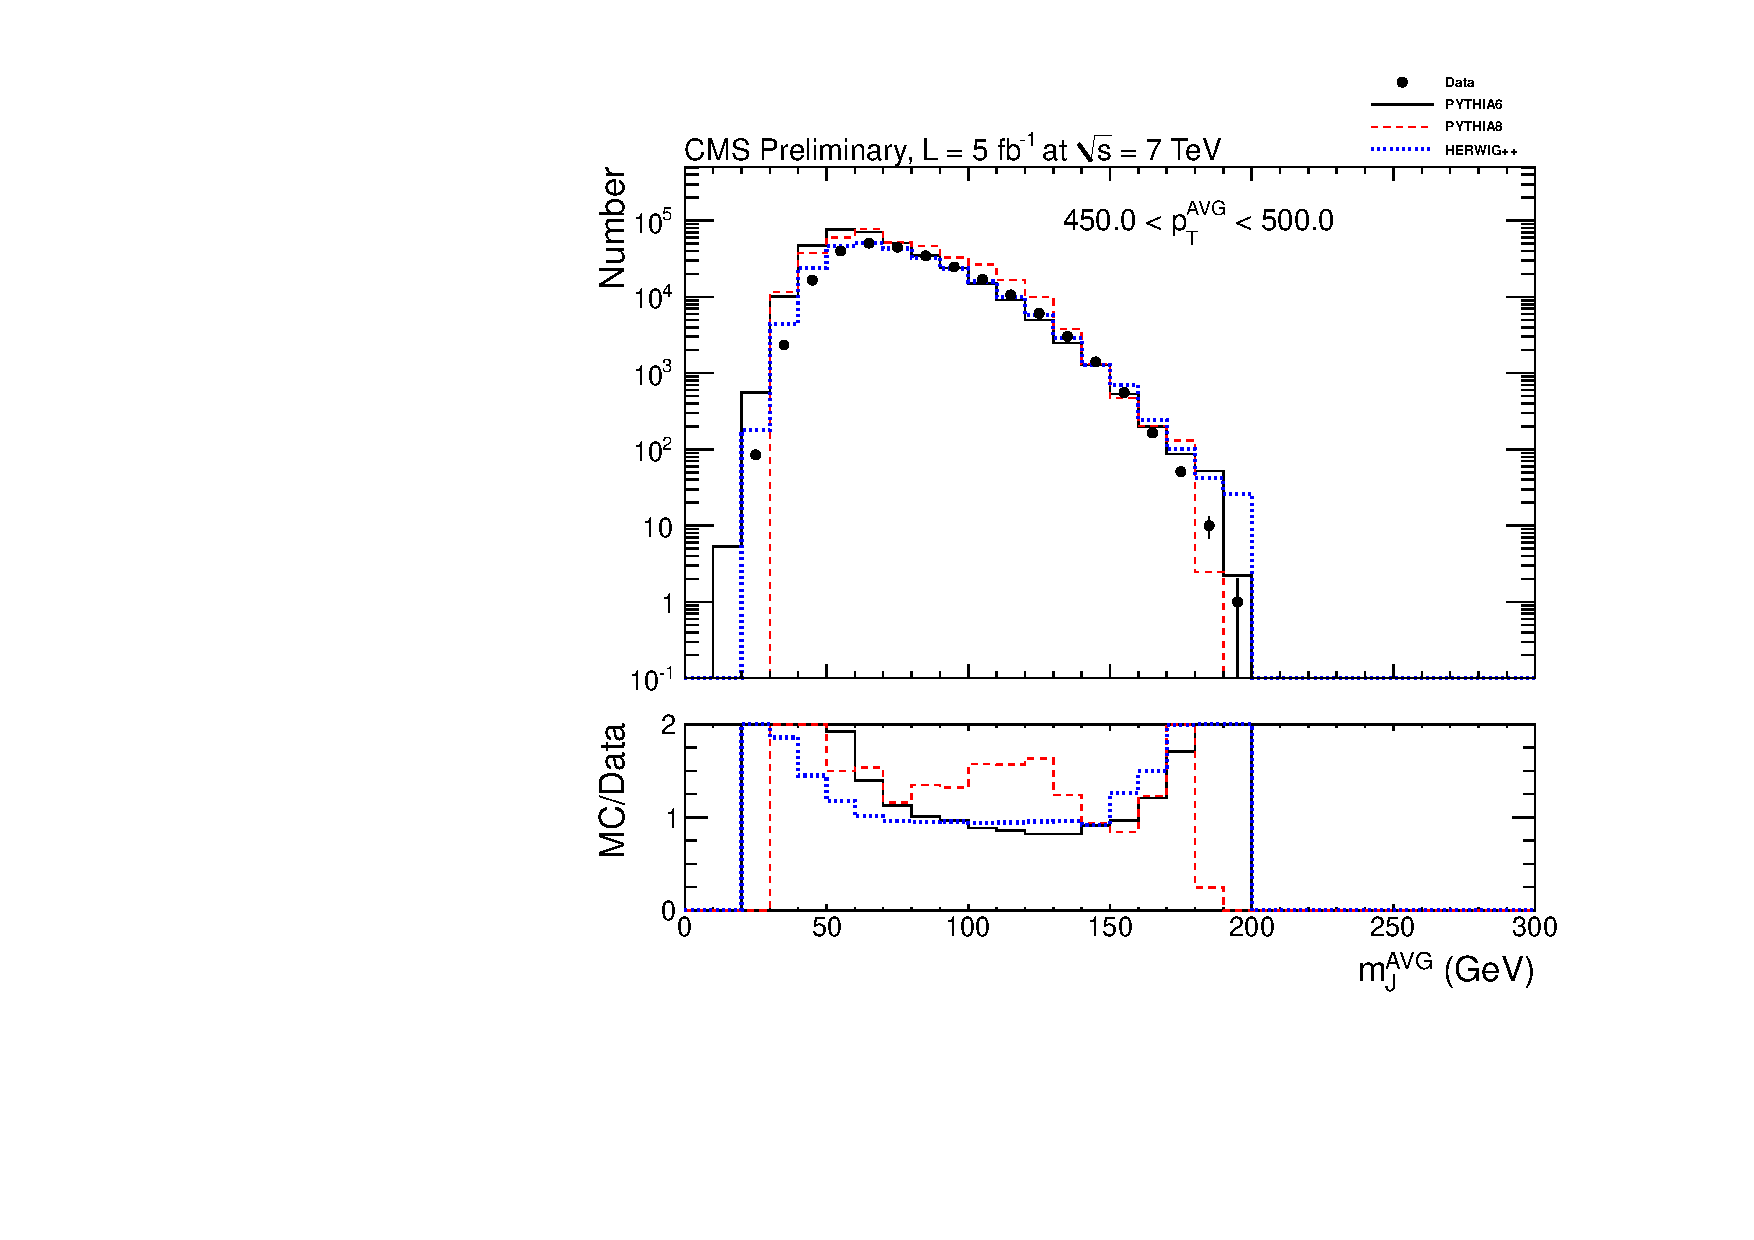
\includegraphics[width=0.95\textwidth]{figs/histAK7MjetVsPtAvg_rawDataMCComparisons_pt_6}
\caption{Detector-level distributions of the jet mass for AK7 jets,
for $450.0 < \pt^{AVG} < 500.0$ \GeVc. The data are shown in black points.
The simulated distribution from \PYTHIA is shown in solid black, 
the from \PYTHIAEIGHT in dashed red, and from \HERWIG in dotted blue. 
The bottom frame shows the ratio of the simulated distribution
to the distribution from data. 
\label{figs:histAK7MjetVsPtAvg_rawDataMCComparisons_pt_6}}
\end{figure}



\begin{figure}[htbp]
\centering
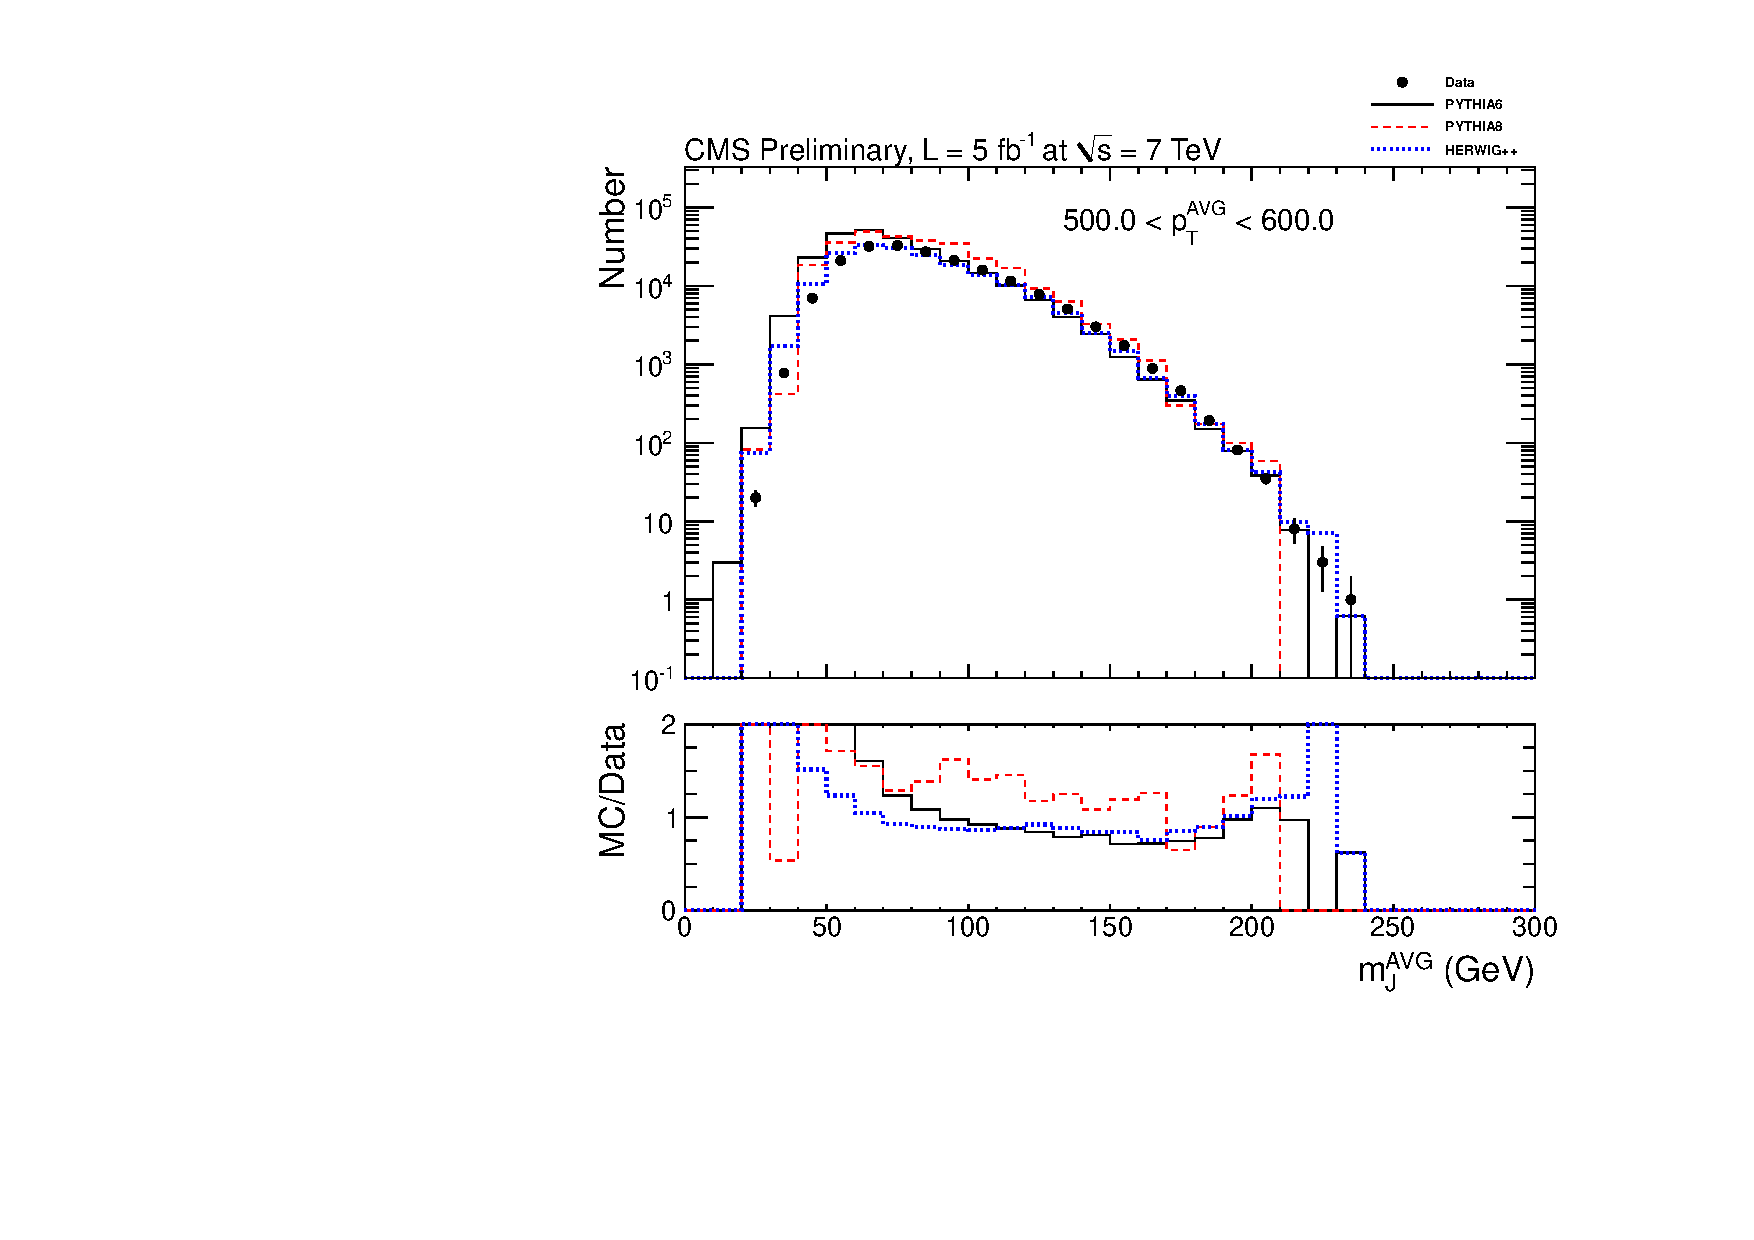
\includegraphics[width=0.95\textwidth]{figs/histAK7MjetVsPtAvg_rawDataMCComparisons_pt_7}
\caption{Detector-level distributions of the jet mass for AK7 jets,
for $500.0 < \pt^{AVG} < 600.0$ \GeVc. The data are shown in black points.
The simulated distribution from \PYTHIA is shown in solid black, 
the from \PYTHIAEIGHT in dashed red, and from \HERWIG in dotted blue. 
The bottom frame shows the ratio of the simulated distribution
to the distribution from data. 
\label{figs:histAK7MjetVsPtAvg_rawDataMCComparisons_pt_7}}
\end{figure}



\begin{figure}[htbp]
\centering
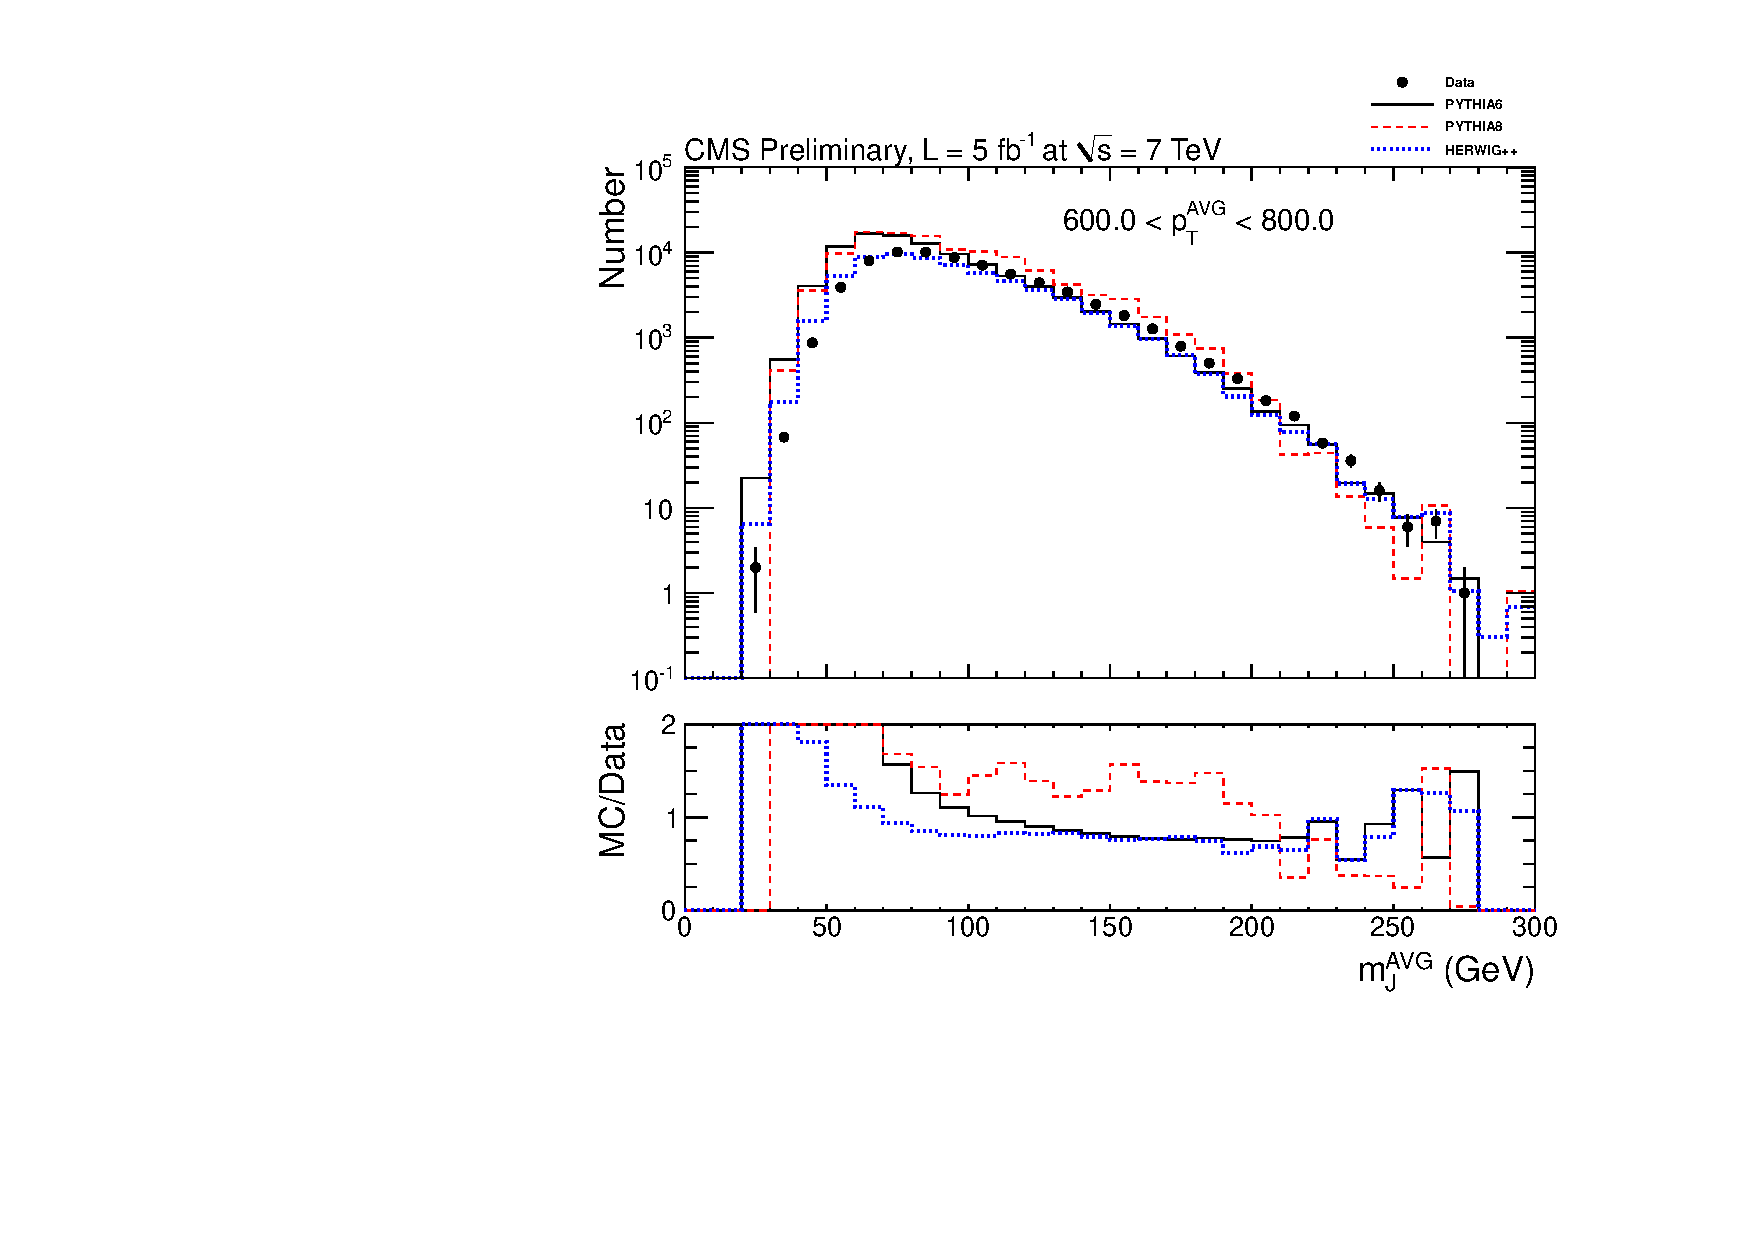
\includegraphics[width=0.95\textwidth]{figs/histAK7MjetVsPtAvg_rawDataMCComparisons_pt_8}
\caption{Detector-level distributions of the jet mass for AK7 jets,
for $600.0 < \pt^{AVG} < 800.0$ \GeVc. The data are shown in black points.
The simulated distribution from \PYTHIA is shown in solid black, 
the from \PYTHIAEIGHT in dashed red, and from \HERWIG in dotted blue. 
The bottom frame shows the ratio of the simulated distribution
to the distribution from data. 
\label{figs:histAK7MjetVsPtAvg_rawDataMCComparisons_pt_8}}
\end{figure}



\begin{figure}[htbp]
\centering
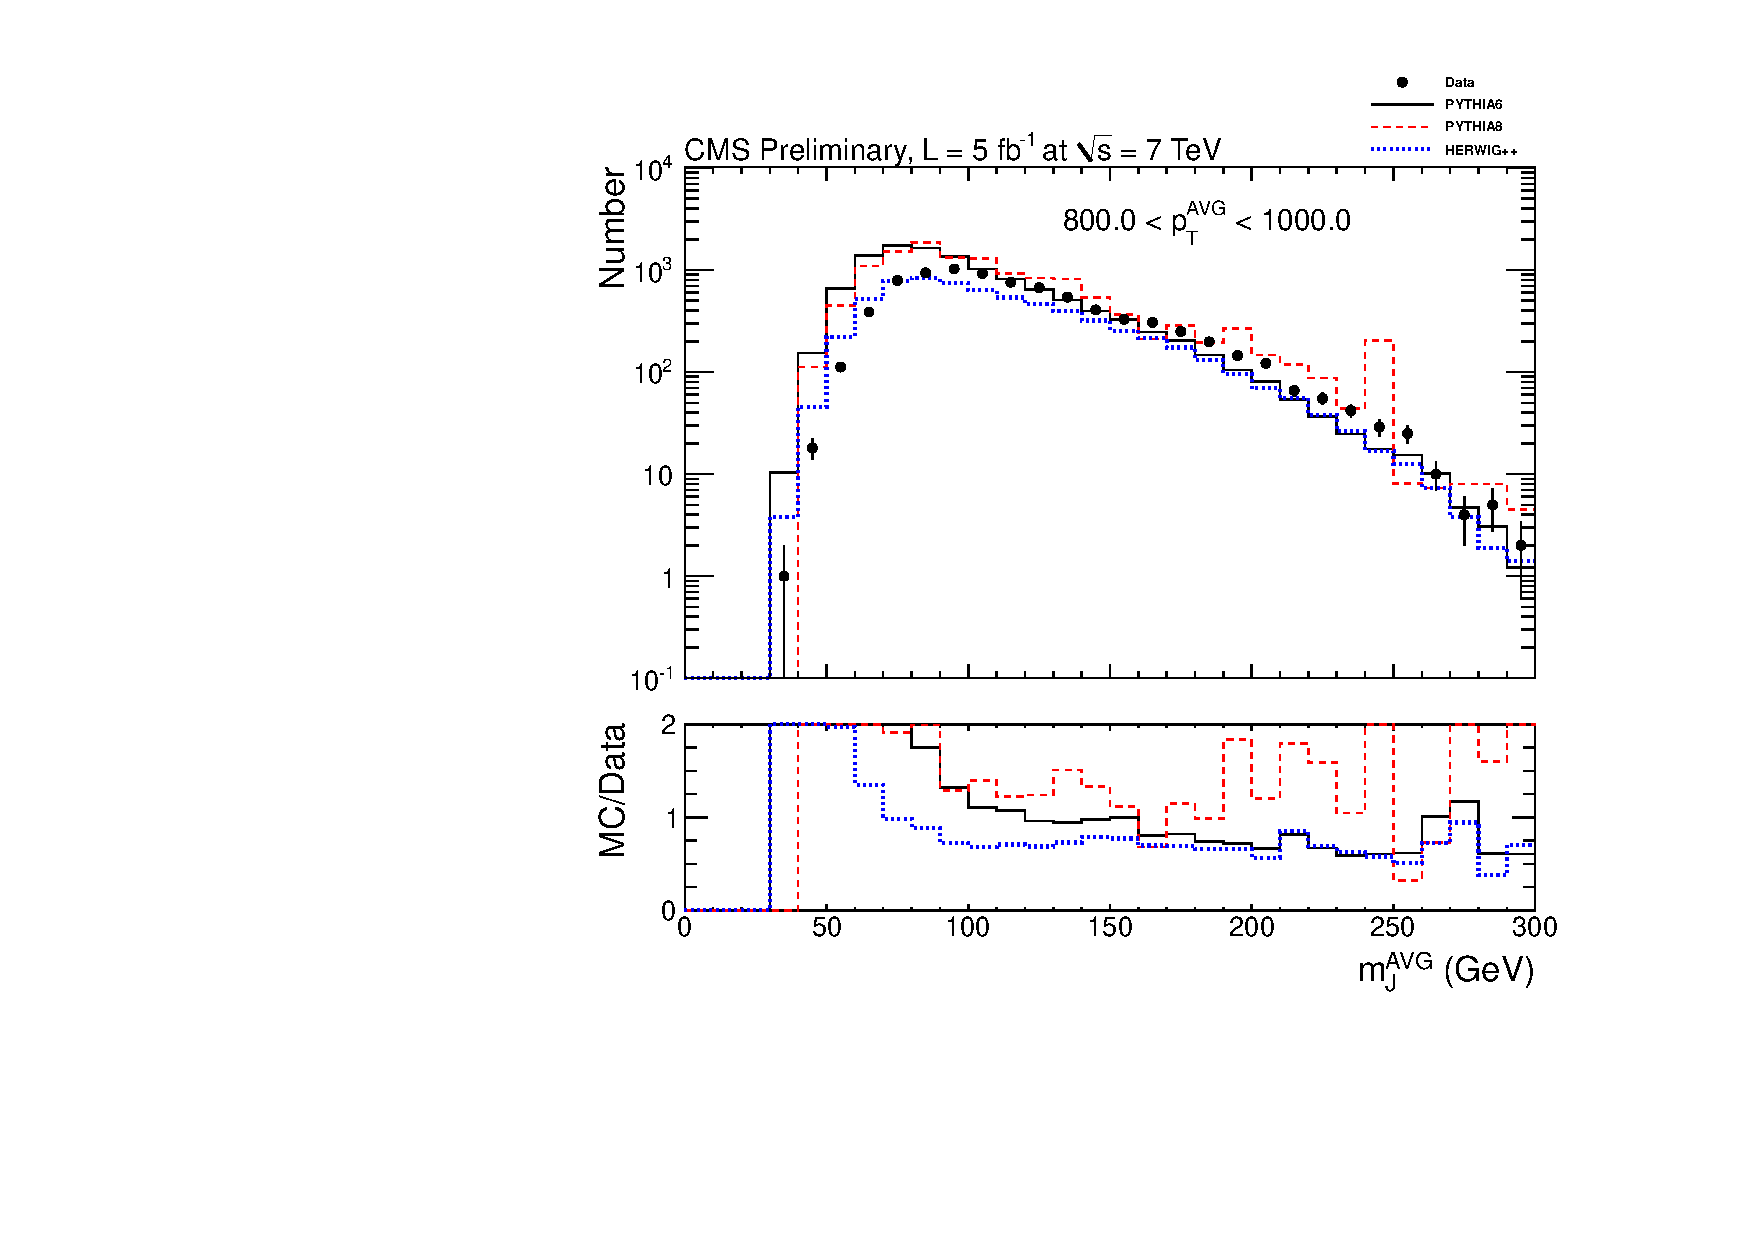
\includegraphics[width=0.95\textwidth]{figs/histAK7MjetVsPtAvg_rawDataMCComparisons_pt_9}
\caption{Detector-level distributions of the jet mass for AK7 jets,
for $800.0 < \pt^{AVG} < 1000.0$ \GeVc. The data are shown in black points.
The simulated distribution from \PYTHIA is shown in solid black, 
the from \PYTHIAEIGHT in dashed red, and from \HERWIG in dotted blue. 
The bottom frame shows the ratio of the simulated distribution
to the distribution from data. 
\label{figs:histAK7MjetVsPtAvg_rawDataMCComparisons_pt_9}}
\end{figure}



\begin{figure}[htbp]
\centering
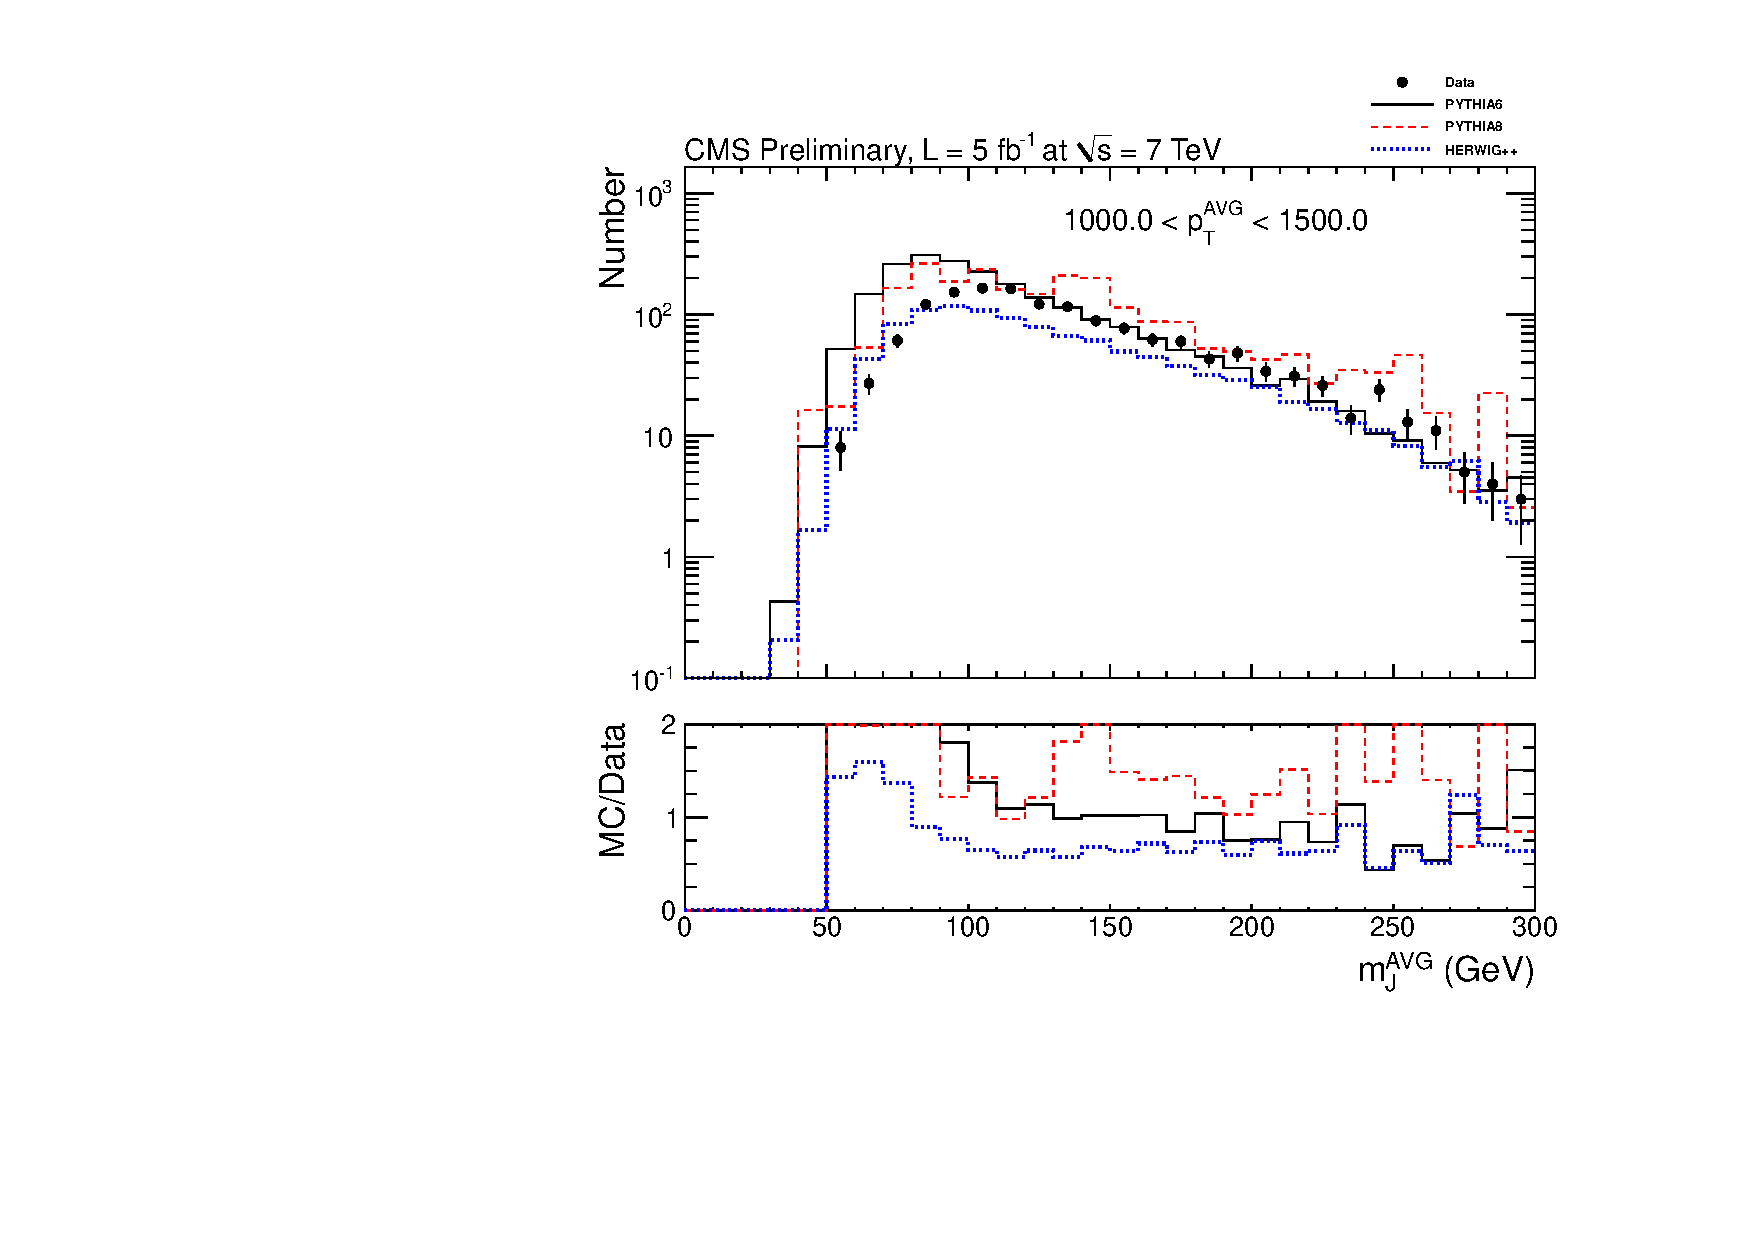
\includegraphics[width=0.95\textwidth]{figs/histAK7MjetVsPtAvg_rawDataMCComparisons_pt_10}
\caption{Detector-level distributions of the jet mass for AK7 jets,
for $1000.0 < \pt^{AVG} < 1500.0$ \GeVc. The data are shown in black points.
The simulated distribution from \PYTHIA is shown in solid black, 
the from \PYTHIAEIGHT in dashed red, and from \HERWIG in dotted blue. 
The bottom frame shows the ratio of the simulated distribution
to the distribution from data. 
\label{figs:histAK7MjetVsPtAvg_rawDataMCComparisons_pt_10}}
\end{figure}

\fi

\clearpage

\ifnpas


\begin{figure}[htbp]
\centering
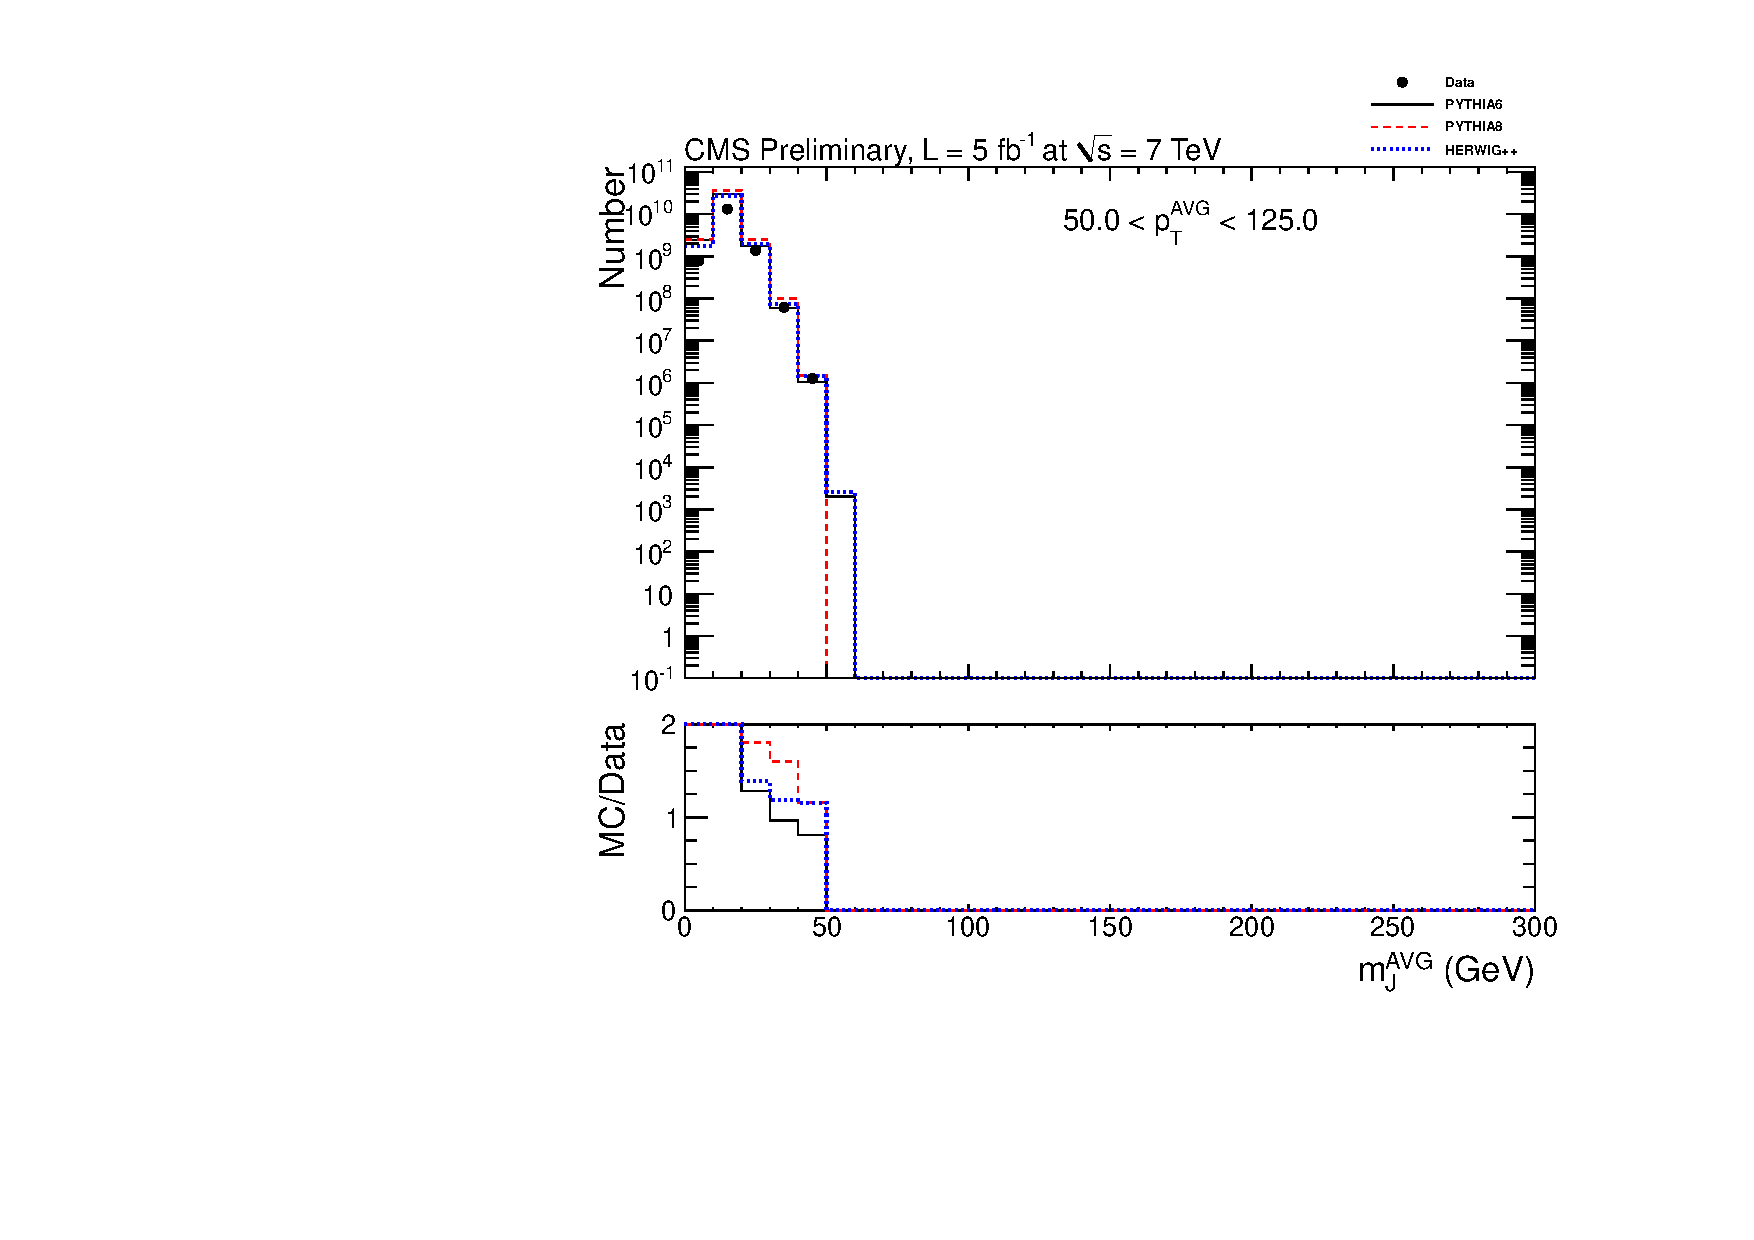
\includegraphics[width=0.95\textwidth]{figs/histAK7MjetVsPtAvg_rawDataMCComparisons_pt_1_Filtered}
\caption{Detector-level distributions of the jet mass for AK7 Filtered jets,
for $50.0 < \pt^{AVG} < 125.0$ \GeVc. The data are shown in black points.
The simulated distribution from \PYTHIA is shown in solid black, 
the from \PYTHIAEIGHT in dashed red, and from \HERWIG in dotted blue. 
The bottom frame shows the ratio of the simulated distribution
to the distribution from data. 
\label{figs:histAK7MjetVsPtAvg_rawDataMCComparisons_pt_1_Filtered}}
\end{figure}

\fi

\begin{figure}[htbp]
\centering
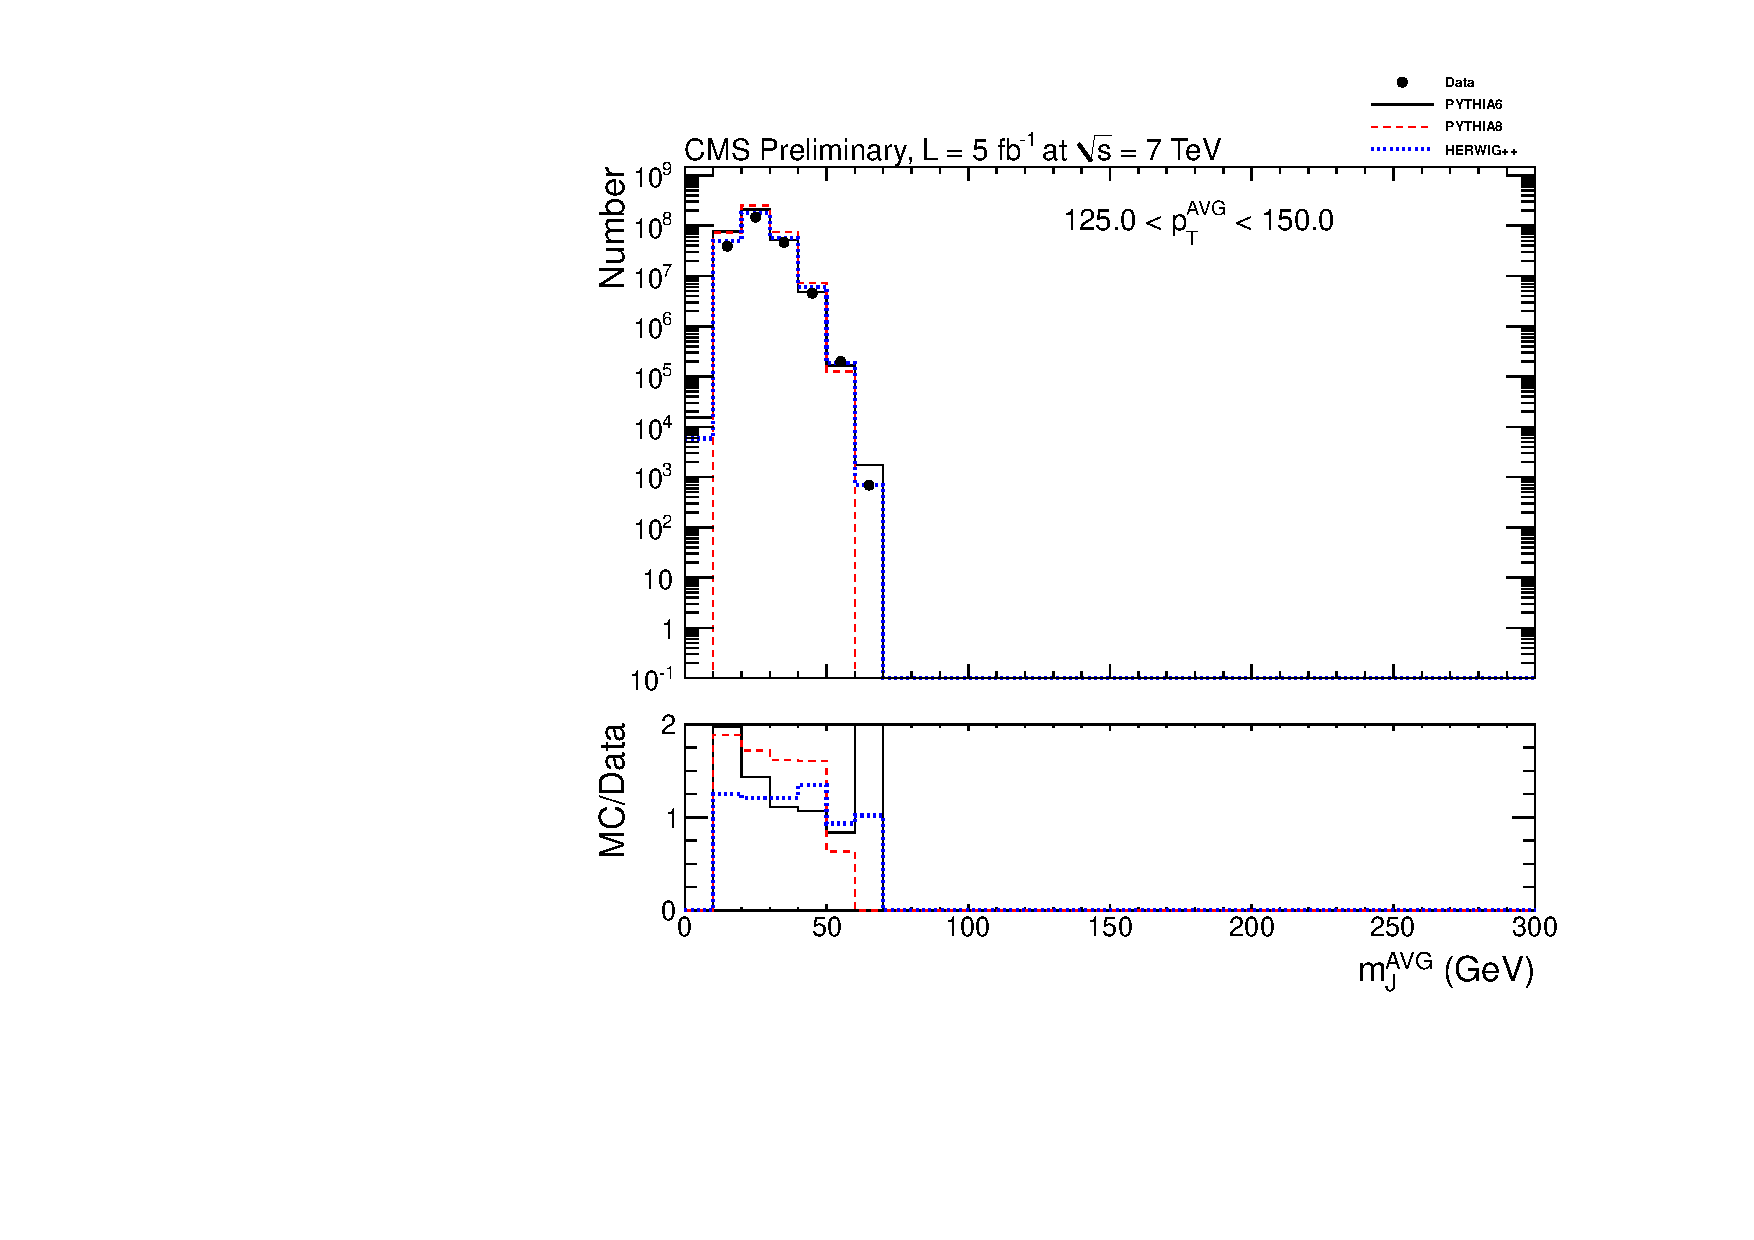
\includegraphics[width=0.49\textwidth]{figs/histAK7MjetVsPtAvg_rawDataMCComparisons_pt_2_Filtered}
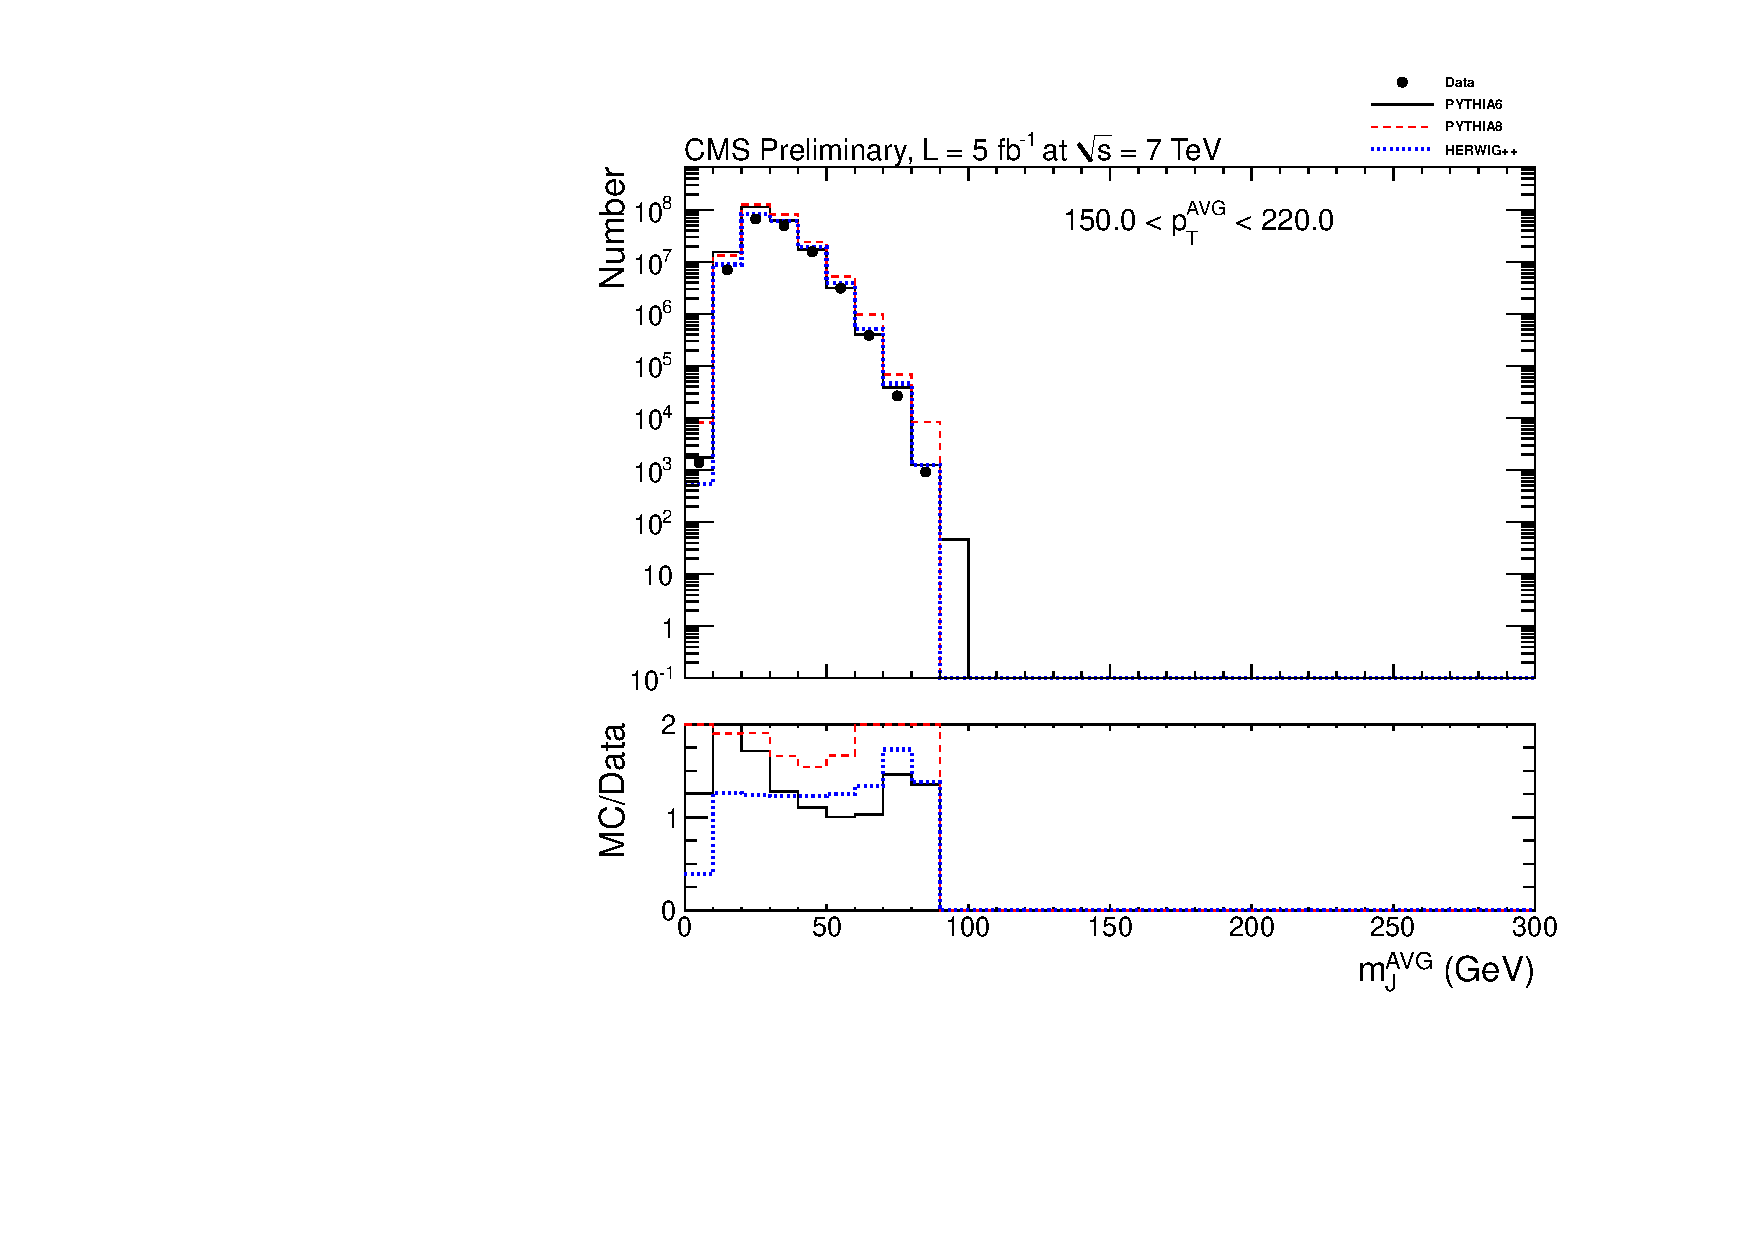
\includegraphics[width=0.49\textwidth]{figs/histAK7MjetVsPtAvg_rawDataMCComparisons_pt_3_Filtered}
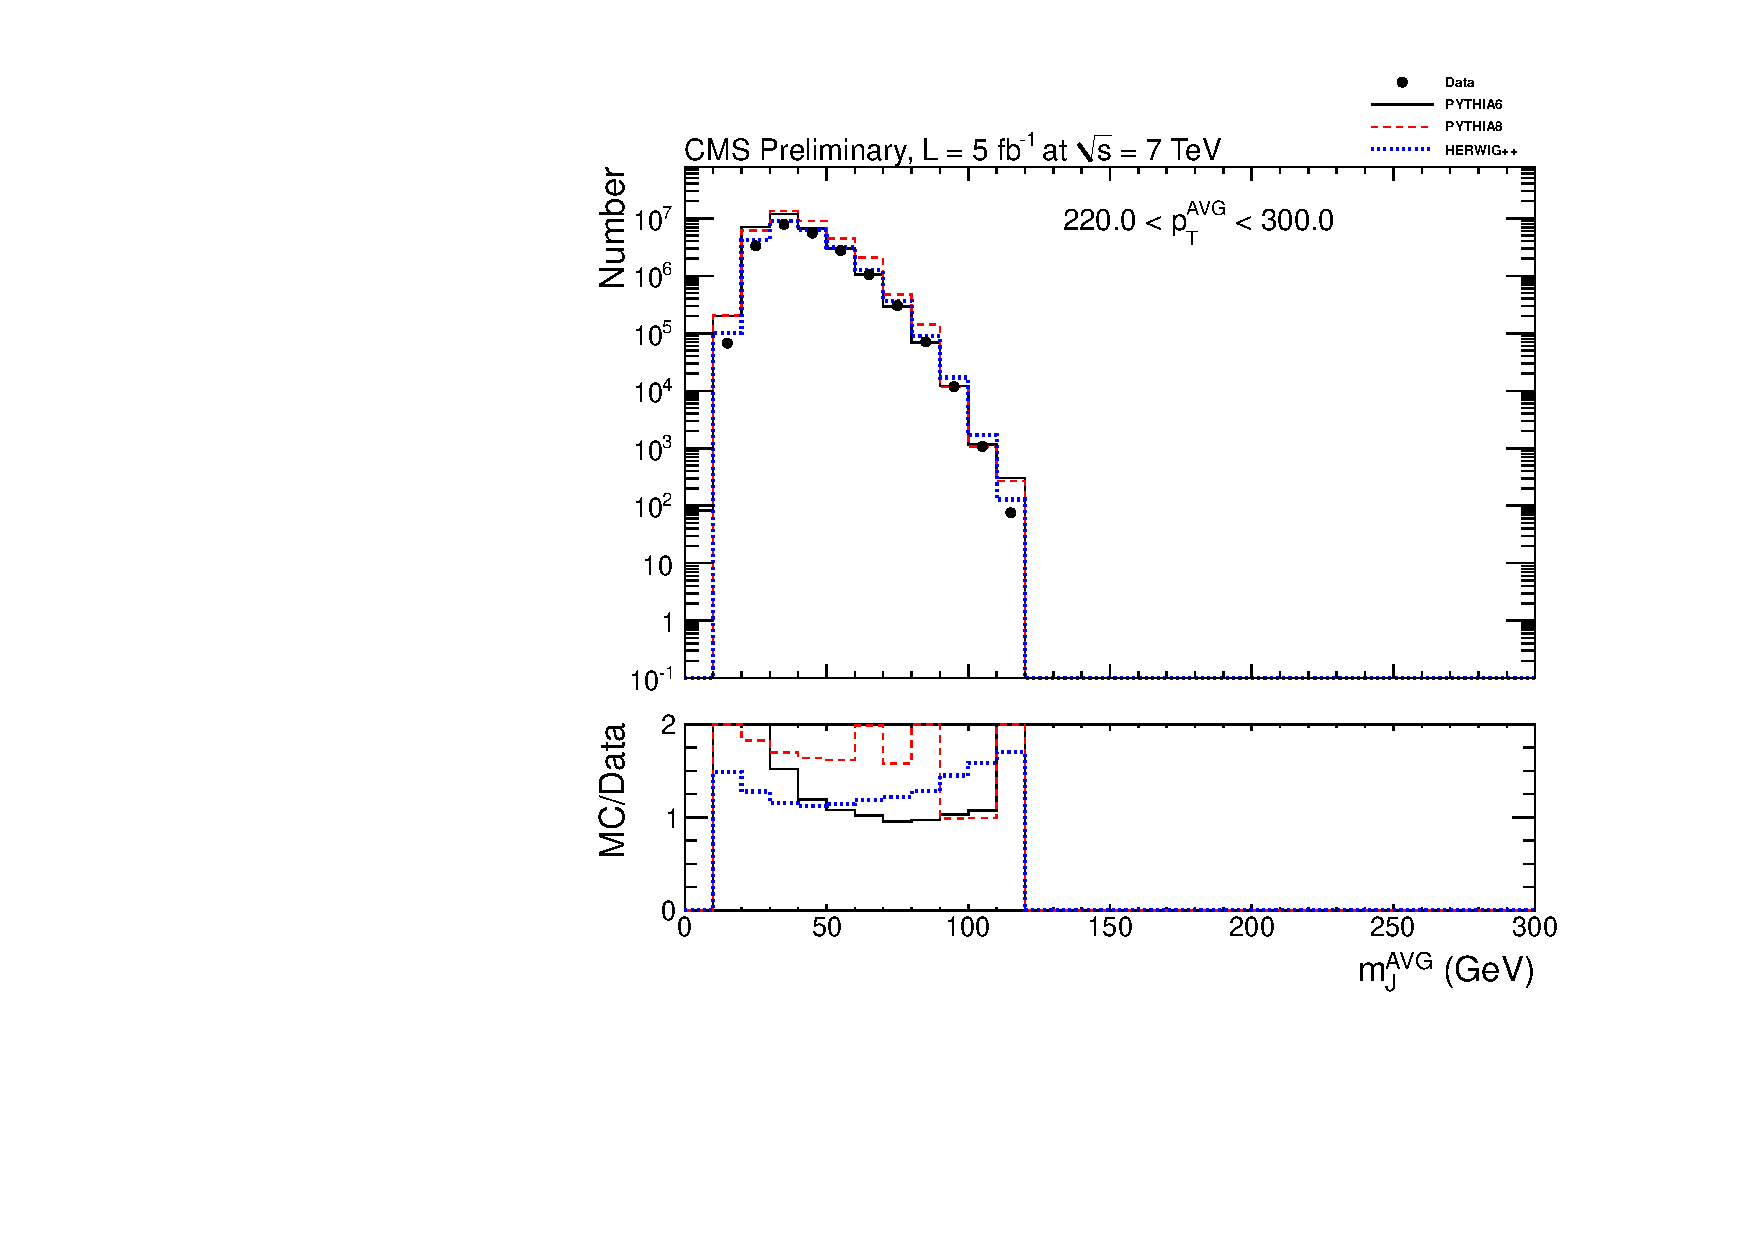
\includegraphics[width=0.49\textwidth]{figs/histAK7MjetVsPtAvg_rawDataMCComparisons_pt_4_Filtered}
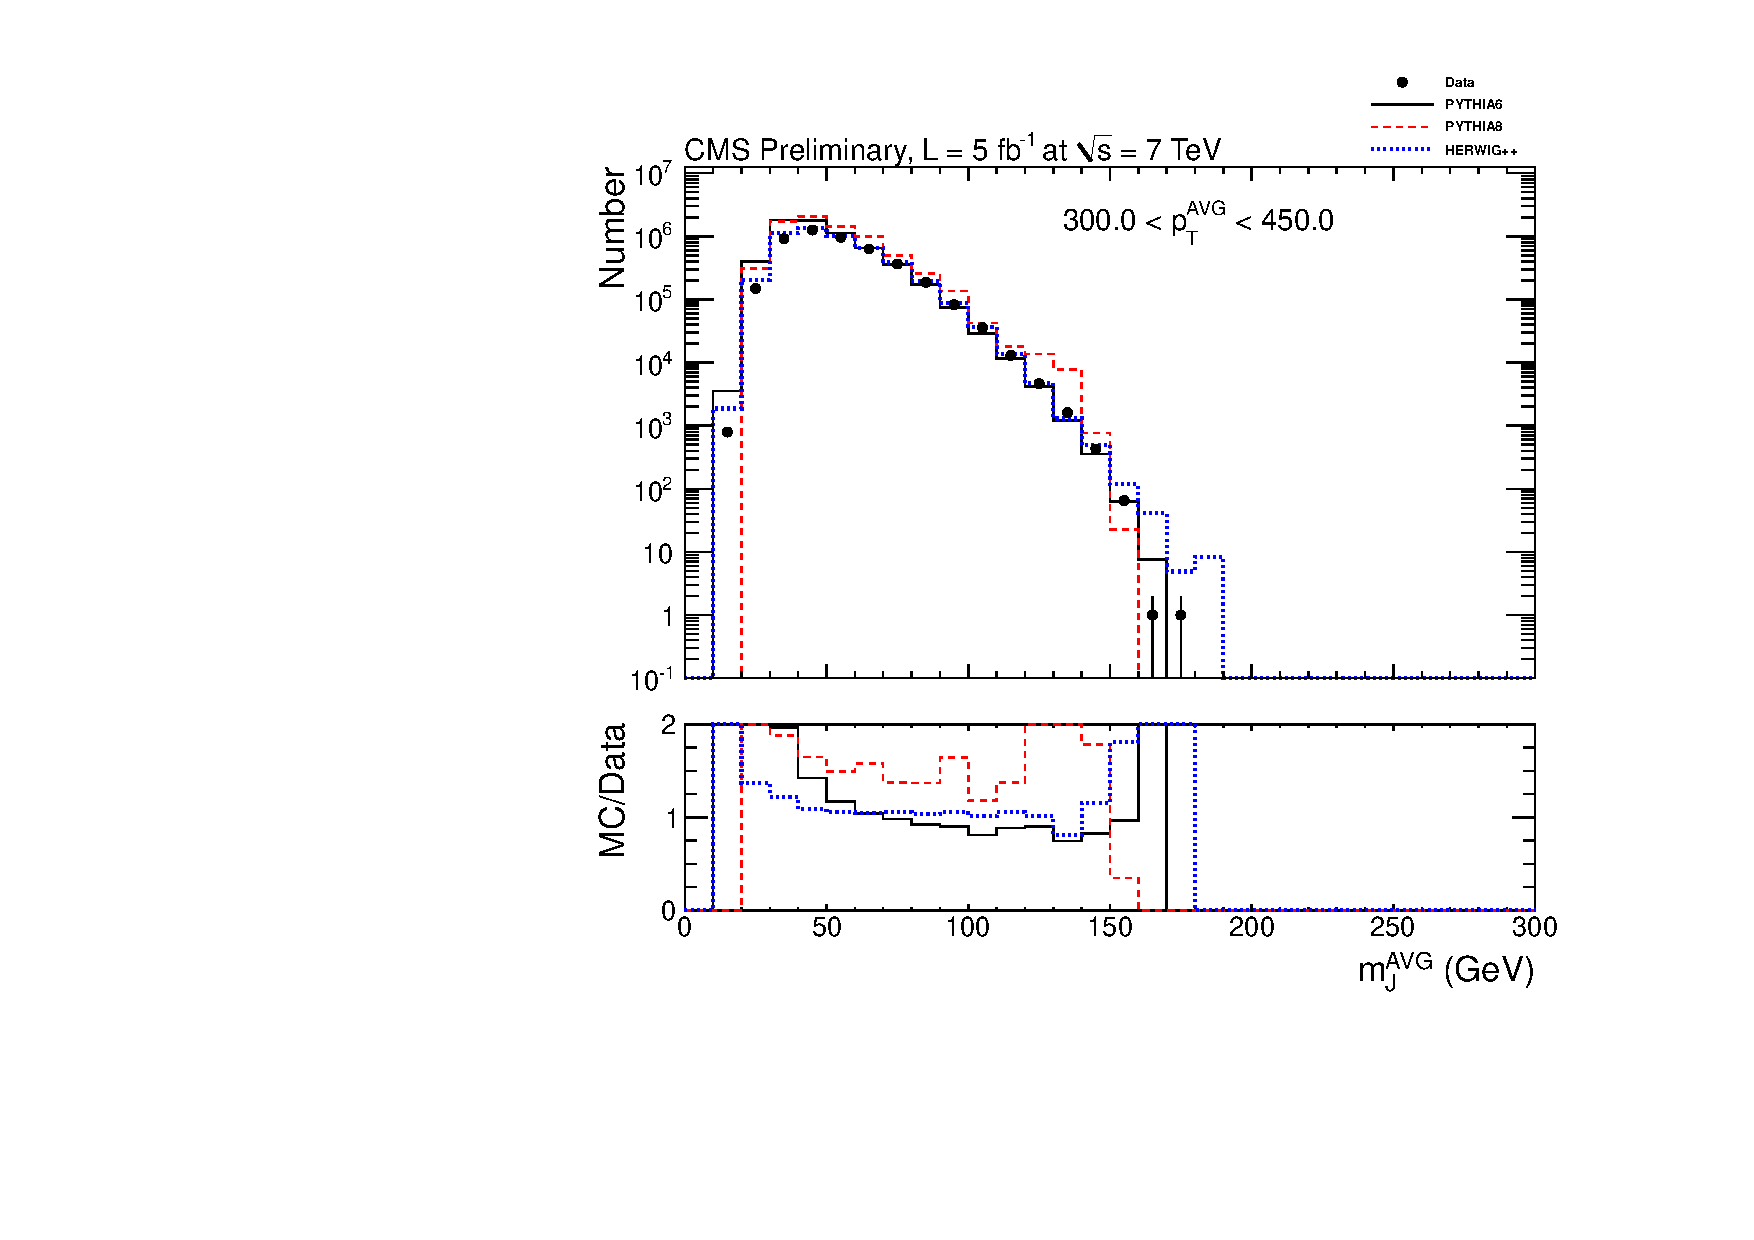
\includegraphics[width=0.49\textwidth]{figs/histAK7MjetVsPtAvg_rawDataMCComparisons_pt_5_Filtered}
\caption{Detector-level distributions of the jet mass for AK7 Filtered jets,
for several $\pt^{AVG}$ bins. The data are shown in black points.
%for $125.0 < \pt^{AVG} < 150.0$ \GeVc. The data are shown in black points.
The simulated distribution from \PYTHIA is shown in solid black, 
the from \PYTHIAEIGHT in dashed red, and from \HERWIG in dotted blue. 
The bottom frame shows the ratio of the simulated distribution
to the distribution from data. 
\label{figs:histAK7MjetVsPtAvg_rawDataMCComparisons_pt_2_Filtered}}
\end{figure}


%%%
\ifnpas

\begin{figure}[htbp]
\centering
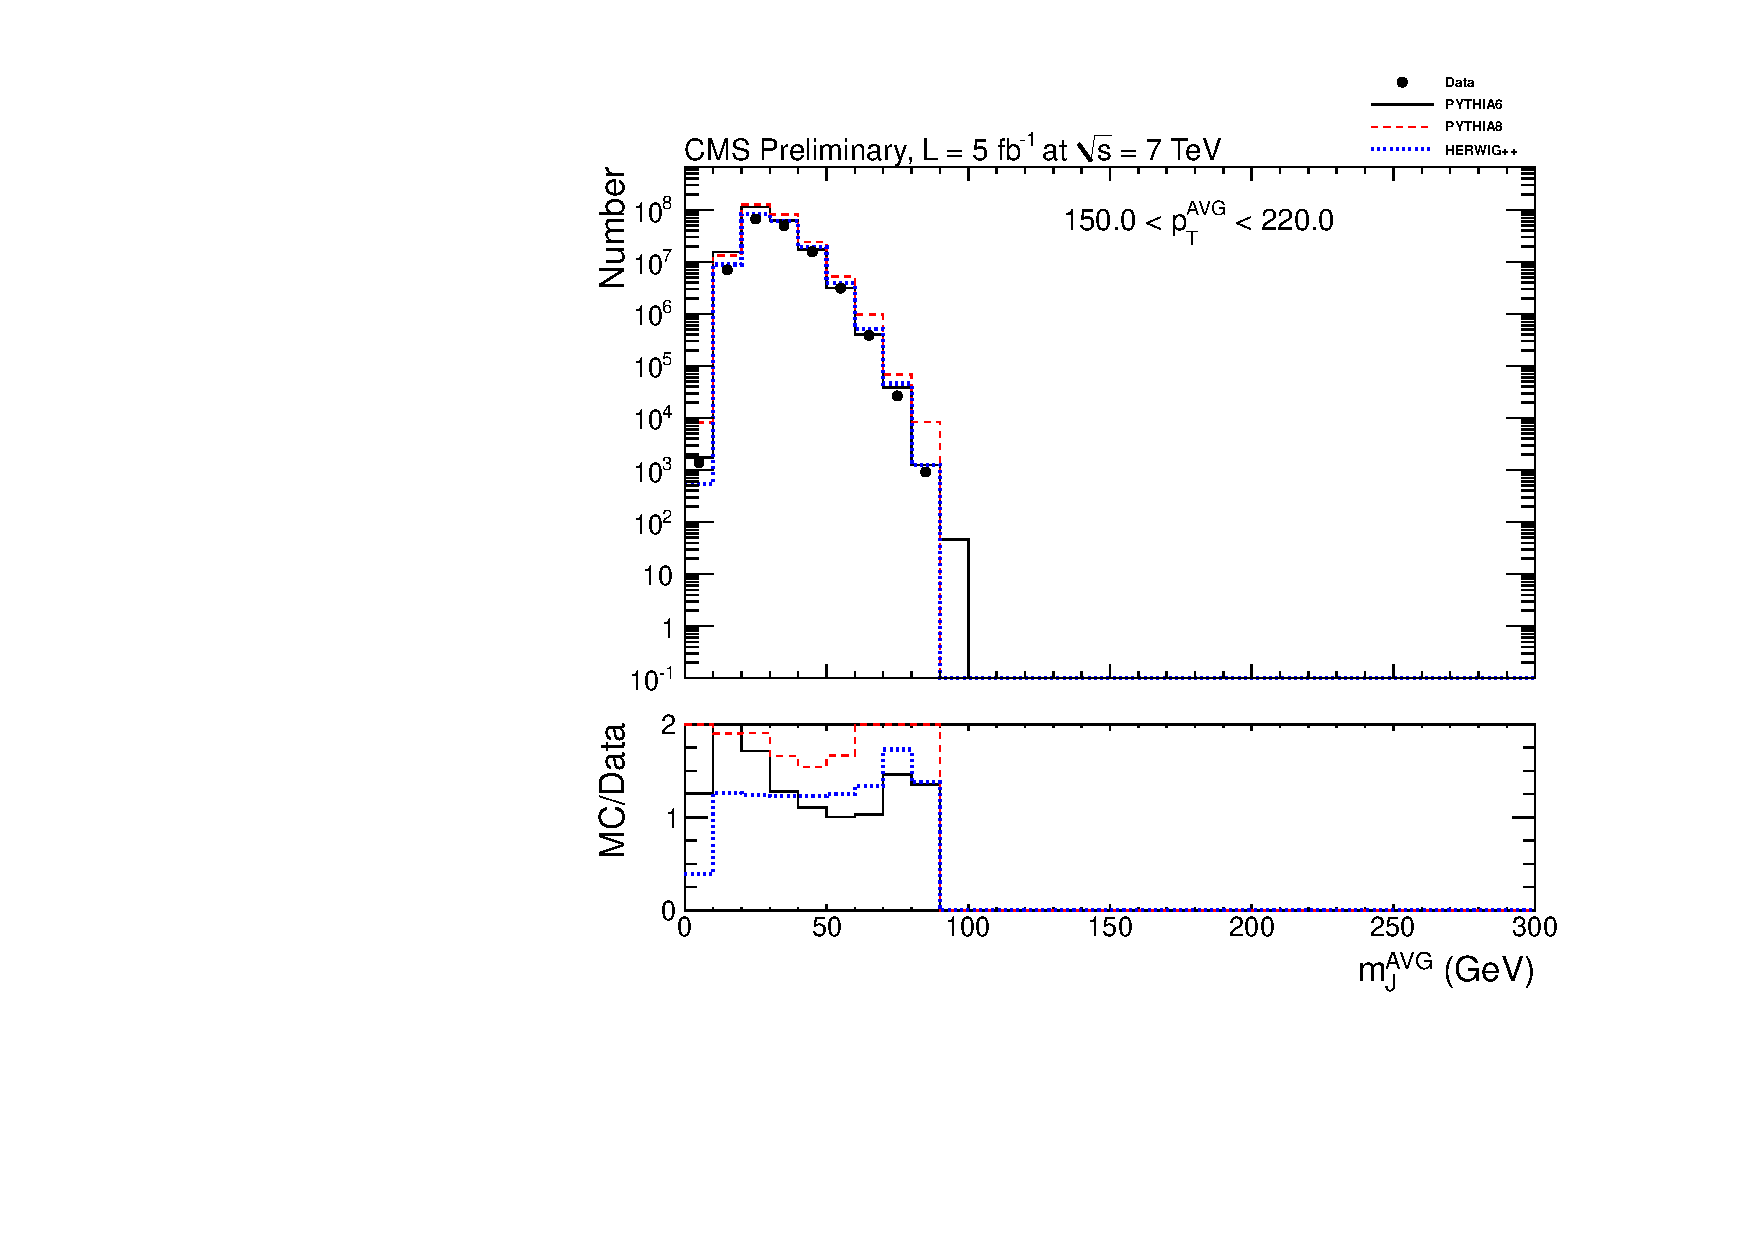
\includegraphics[width=0.95\textwidth]{figs/histAK7MjetVsPtAvg_rawDataMCComparisons_pt_3_Filtered}
\caption{Detector-level distributions of the jet mass for AK7 Filtered jets,
for $150.0 < \pt^{AVG} < 220.0$ \GeVc. The data are shown in black points.
The simulated distribution from \PYTHIA is shown in solid black, 
the from \PYTHIAEIGHT in dashed red, and from \HERWIG in dotted blue. 
The bottom frame shows the ratio of the simulated distribution
to the distribution from data. 
\label{figs:histAK7MjetVsPtAvg_rawDataMCComparisons_pt_3_Filtered}}
\end{figure}



\begin{figure}[htbp]
\centering
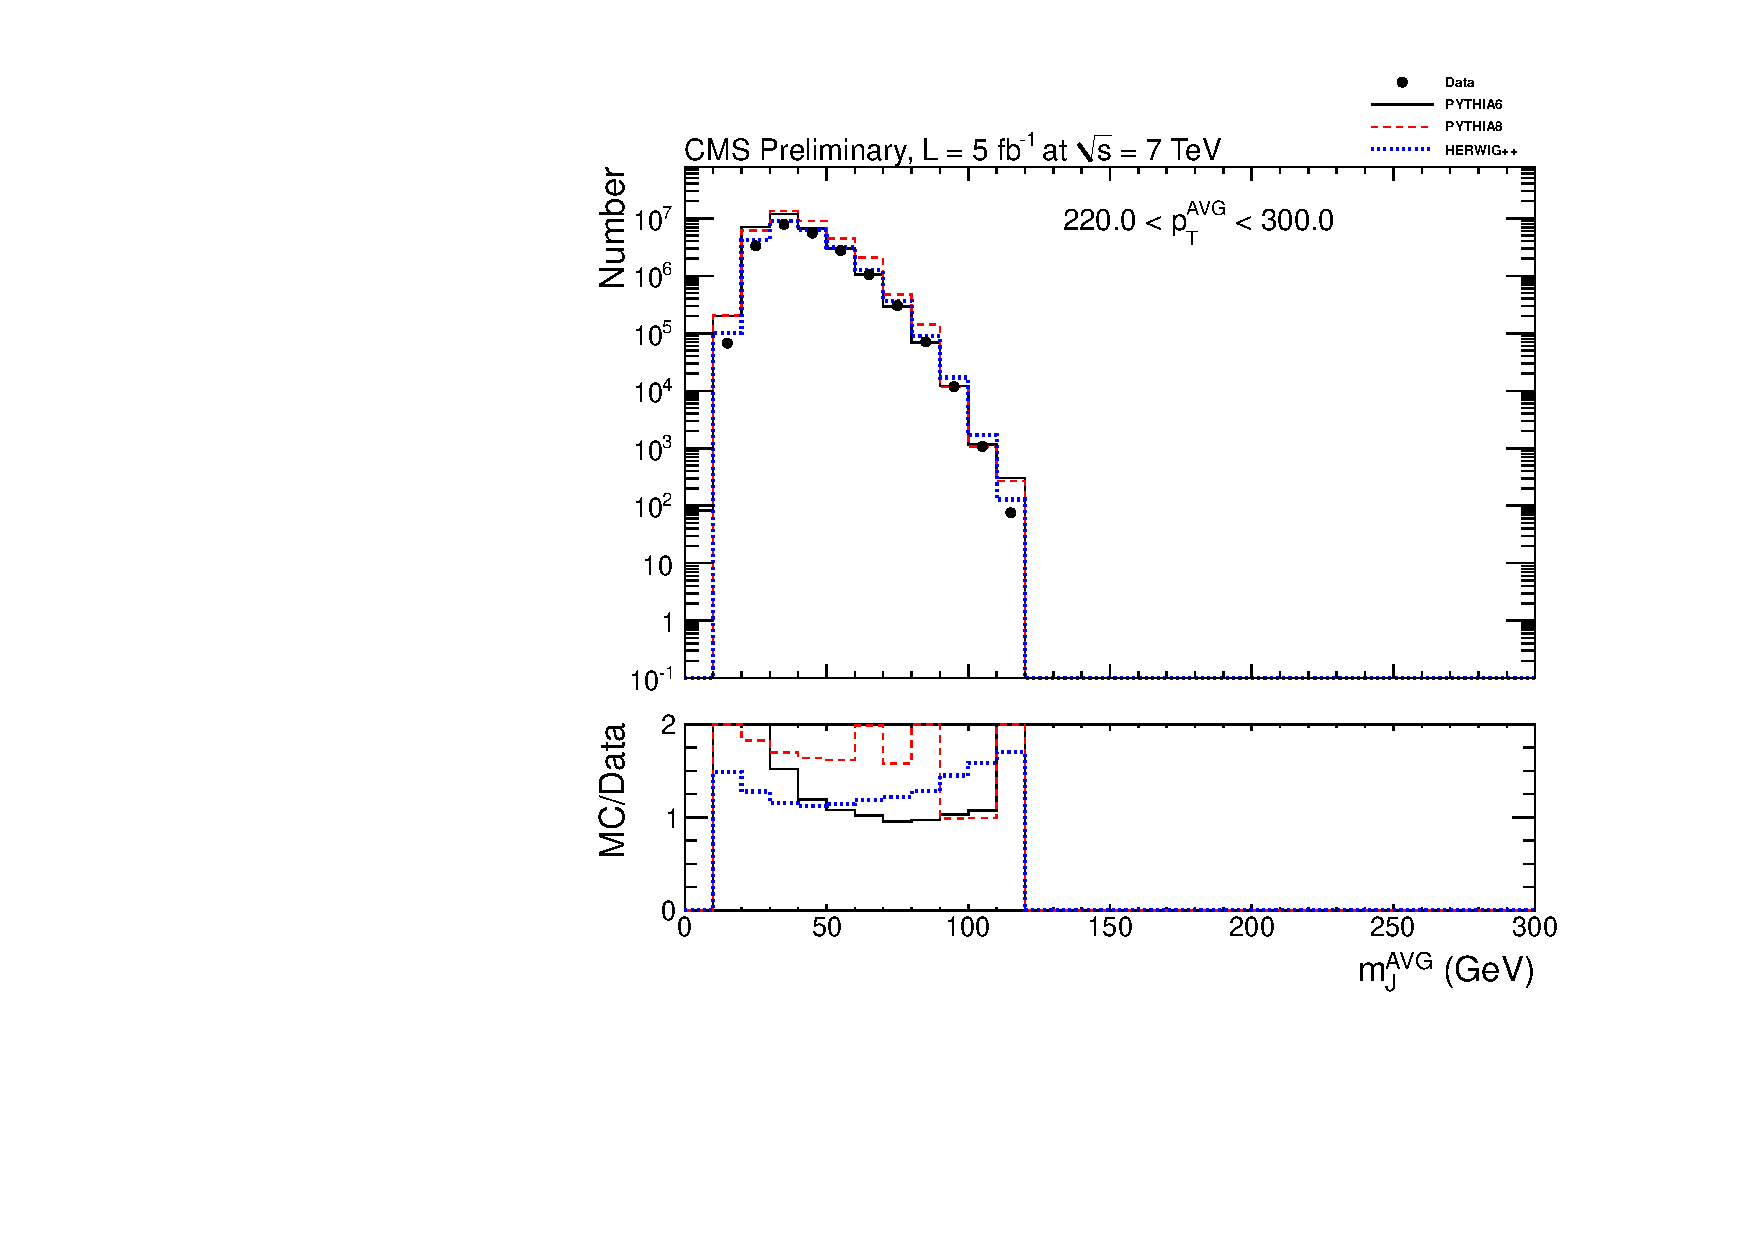
\includegraphics[width=0.95\textwidth]{figs/histAK7MjetVsPtAvg_rawDataMCComparisons_pt_4_Filtered}
\caption{Detector-level distributions of the jet mass for AK7 Filtered jets,
for $220.0 < \pt^{AVG} < 300.0$ \GeVc. The data are shown in black points.
The simulated distribution from \PYTHIA is shown in solid black, 
the from \PYTHIAEIGHT in dashed red, and from \HERWIG in dotted blue. 
The bottom frame shows the ratio of the simulated distribution
to the distribution from data. 
\label{figs:histAK7MjetVsPtAvg_rawDataMCComparisons_pt_4_Filtered}}
\end{figure}



\begin{figure}[htbp]
\centering
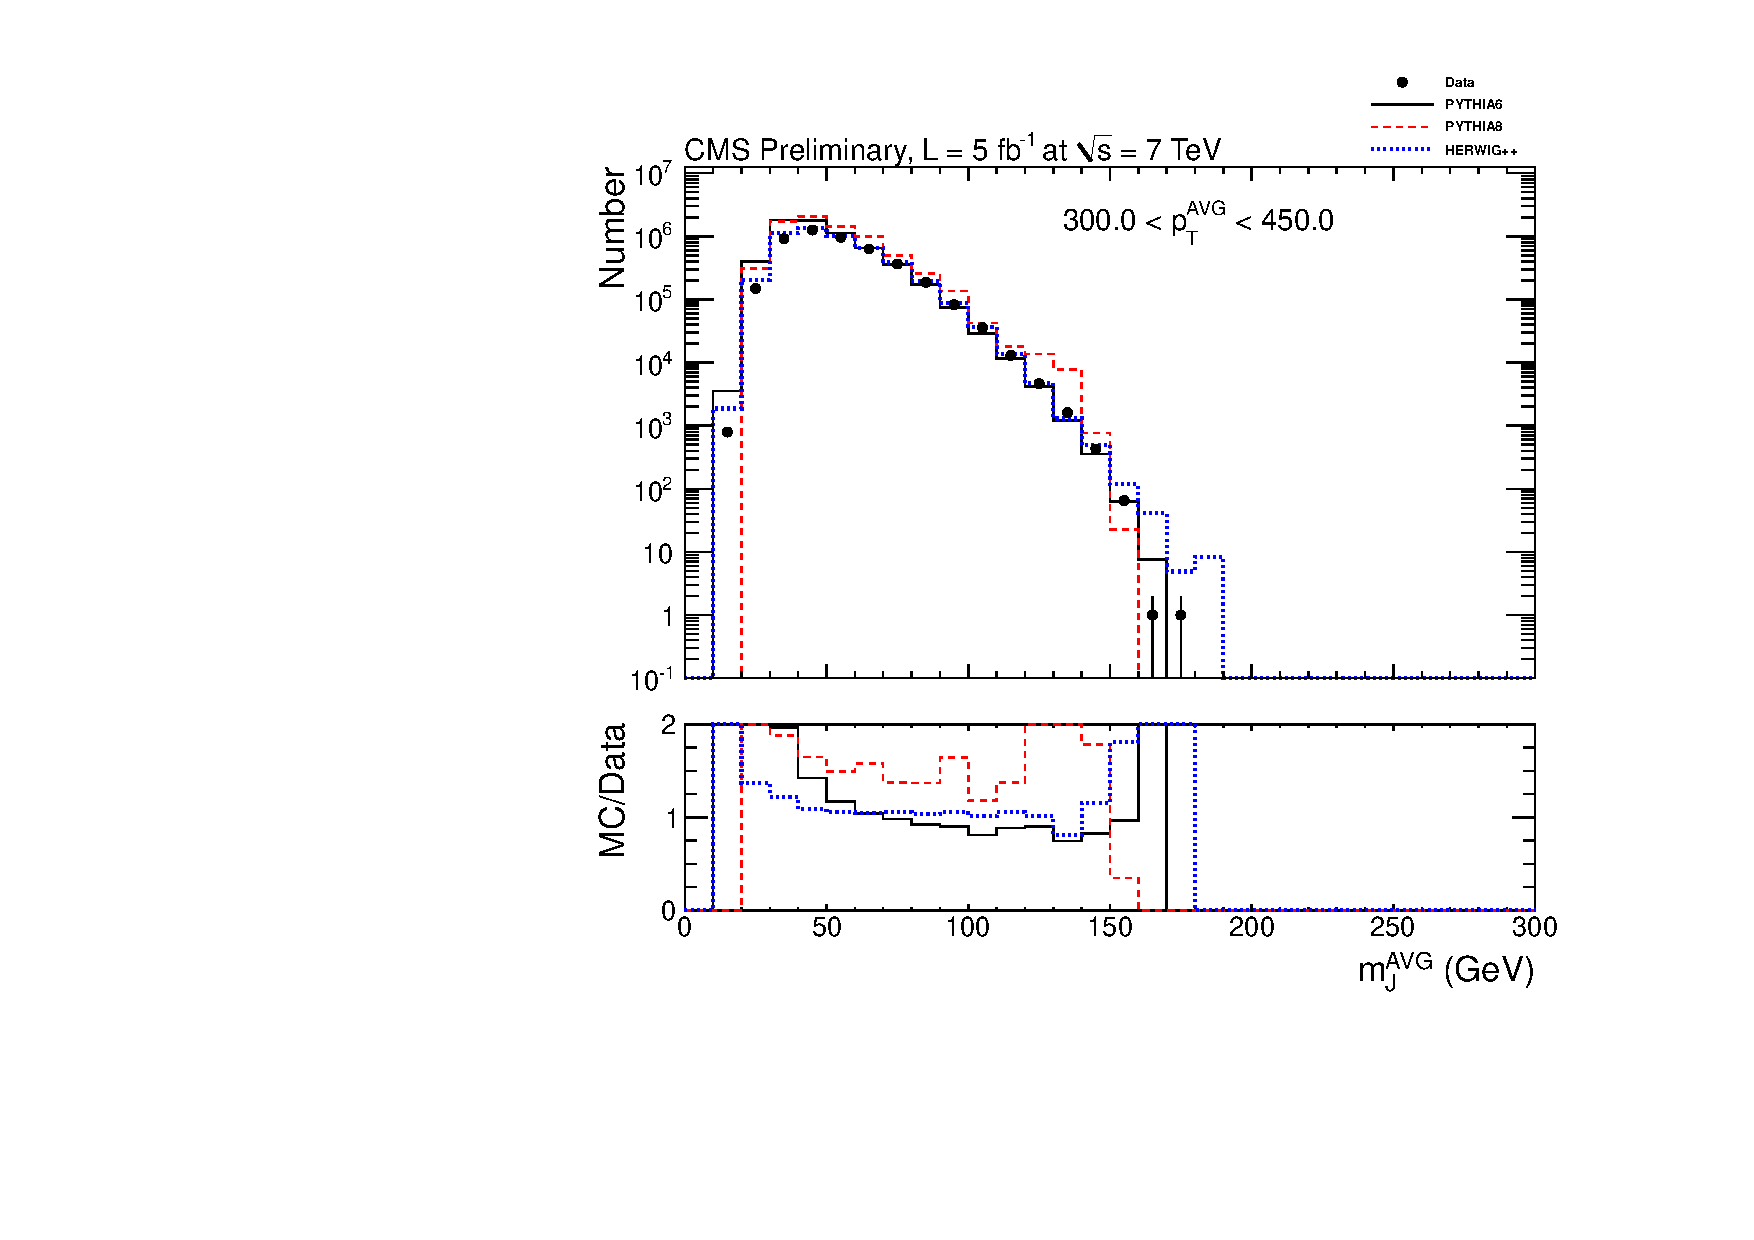
\includegraphics[width=0.95\textwidth]{figs/histAK7MjetVsPtAvg_rawDataMCComparisons_pt_5_Filtered}
\caption{Detector-level distributions of the jet mass for AK7 Filtered jets,
for $300.0 < \pt^{AVG} < 450.0$ \GeVc. The data are shown in black points.
The simulated distribution from \PYTHIA is shown in solid black, 
the from \PYTHIAEIGHT in dashed red, and from \HERWIG in dotted blue. 
The bottom frame shows the ratio of the simulated distribution
to the distribution from data. 
\label{figs:histAK7MjetVsPtAvg_rawDataMCComparisons_pt_5_Filtered}}
\end{figure}

\fi
%%%%%%%

\ifnpas

\begin{figure}[htbp]
\centering
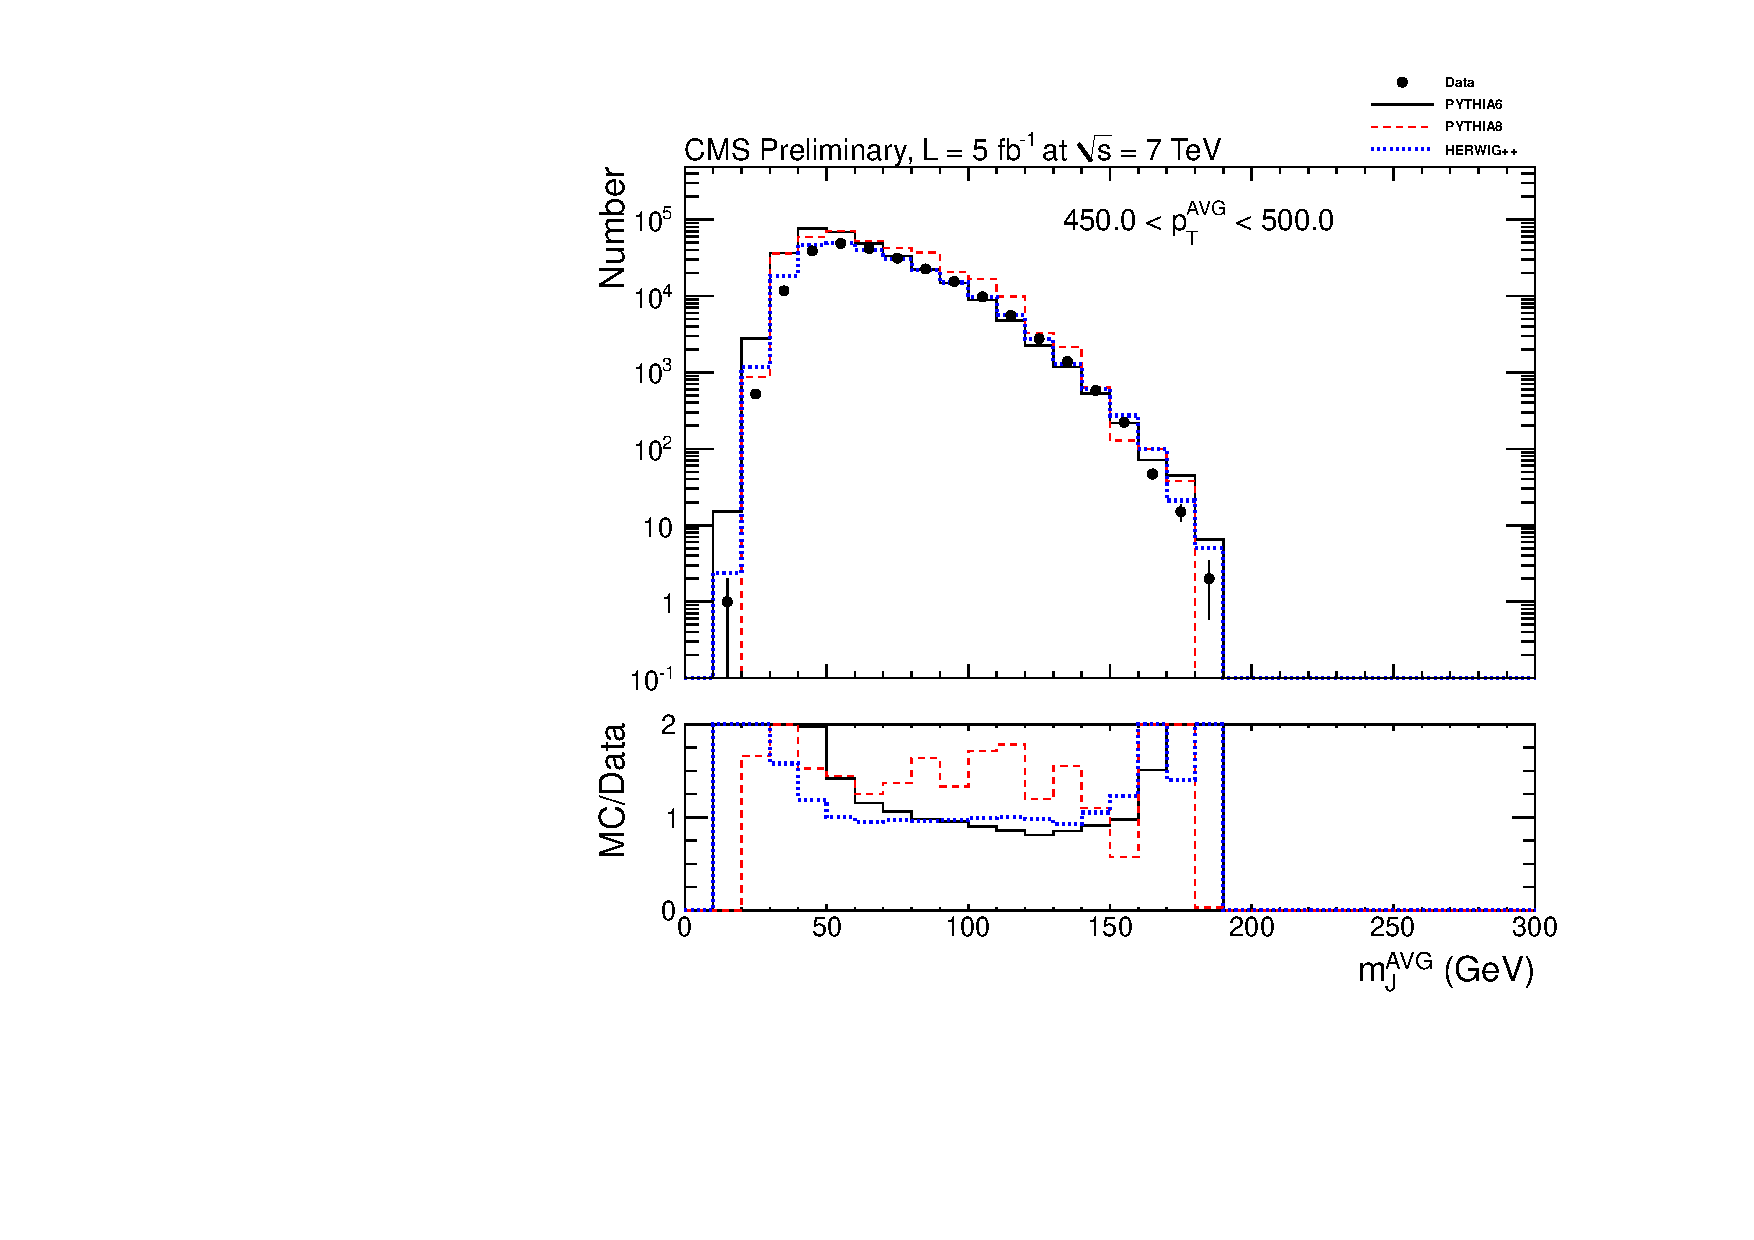
\includegraphics[width=0.95\textwidth]{figs/histAK7MjetVsPtAvg_rawDataMCComparisons_pt_6_Filtered}
\caption{Detector-level distributions of the jet mass for AK7 Filtered jets,
for $450.0 < \pt^{AVG} < 500.0$ \GeVc. The data are shown in black points.
The simulated distribution from \PYTHIA is shown in solid black, 
the from \PYTHIAEIGHT in dashed red, and from \HERWIG in dotted blue. 
The bottom frame shows the ratio of the simulated distribution
to the distribution from data. 
\label{figs:histAK7MjetVsPtAvg_rawDataMCComparisons_pt_6_Filtered}}
\end{figure}



\begin{figure}[htbp]
\centering
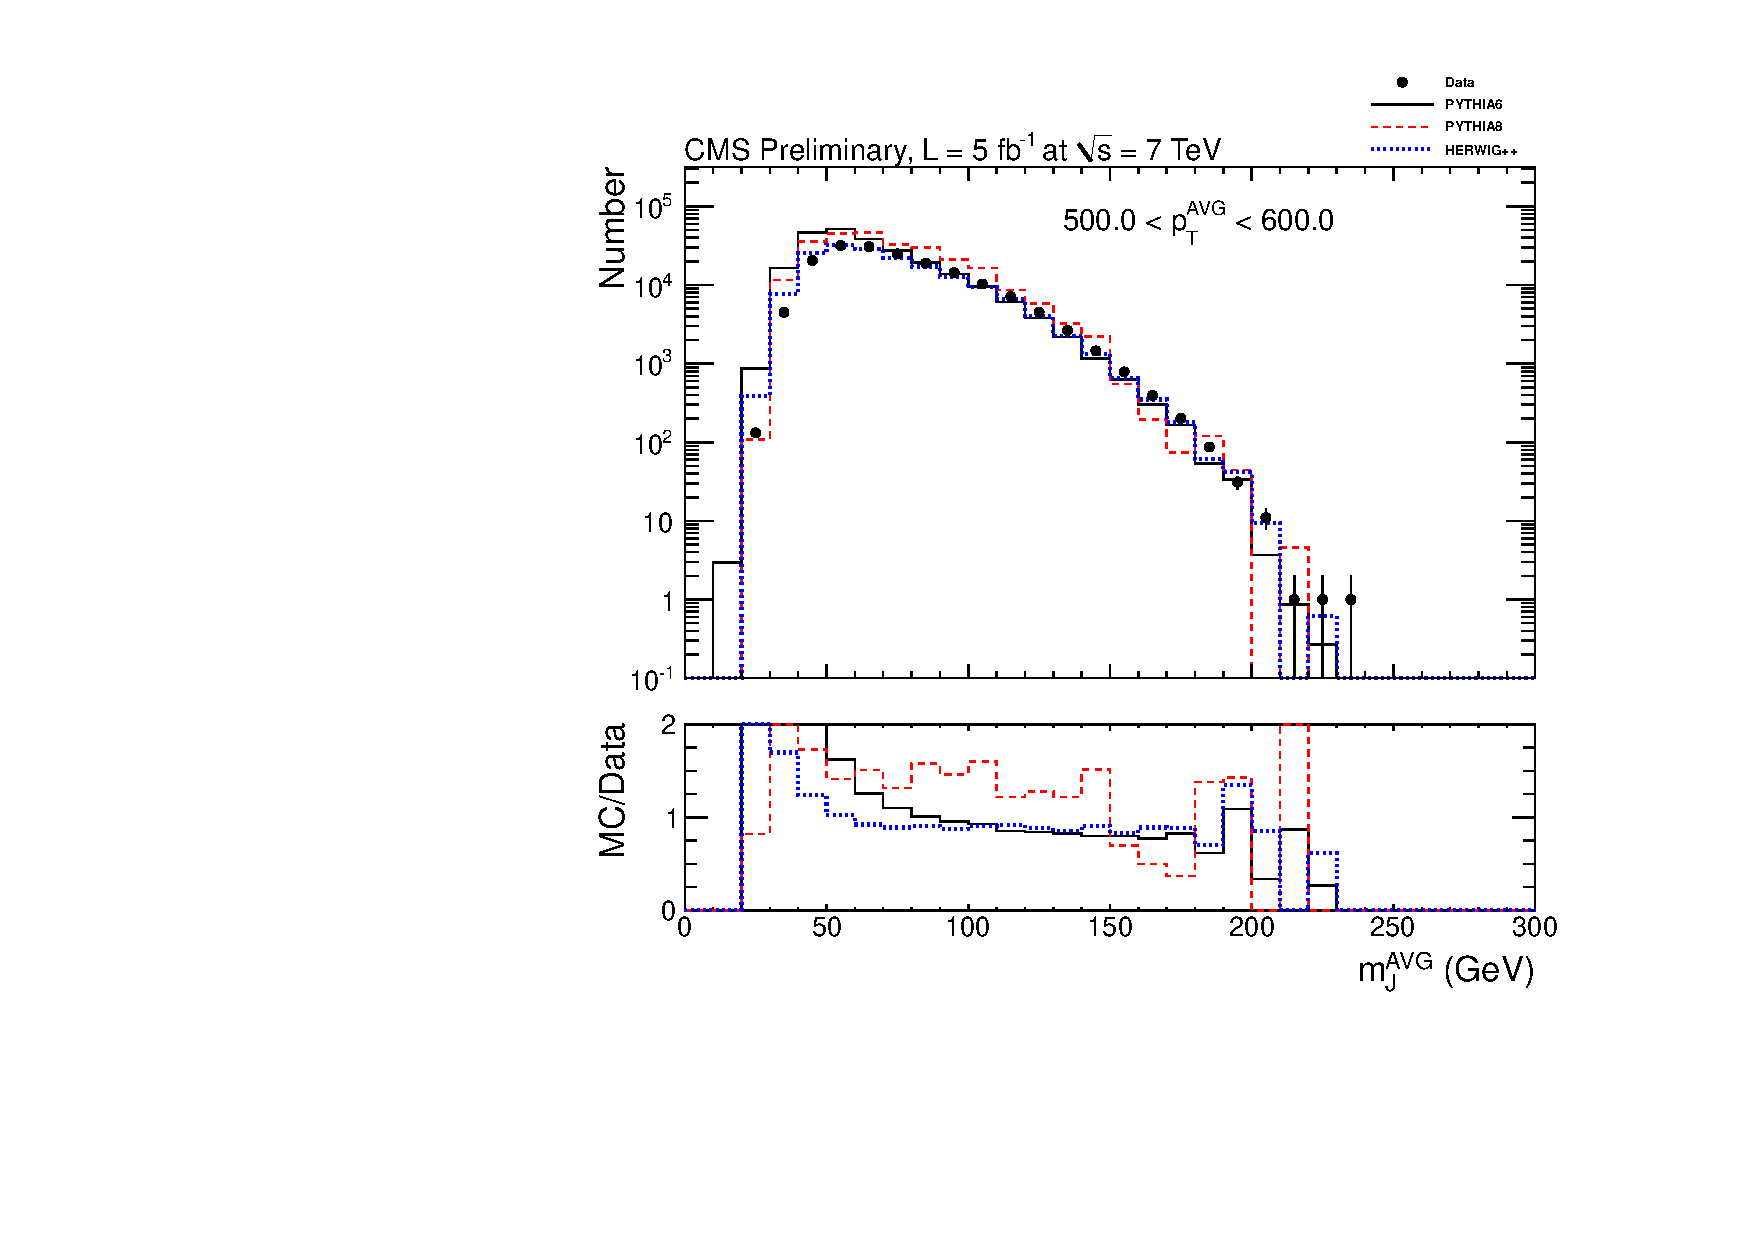
\includegraphics[width=0.95\textwidth]{figs/histAK7MjetVsPtAvg_rawDataMCComparisons_pt_7_Filtered}
\caption{Detector-level distributions of the jet mass for AK7 Filtered jets,
for $500.0 < \pt^{AVG} < 600.0$ \GeVc. The data are shown in black points.
The simulated distribution from \PYTHIA is shown in solid black, 
the from \PYTHIAEIGHT in dashed red, and from \HERWIG in dotted blue. 
The bottom frame shows the ratio of the simulated distribution
to the distribution from data. 
\label{figs:histAK7MjetVsPtAvg_rawDataMCComparisons_pt_7_Filtered}}
\end{figure}



\begin{figure}[htbp]
\centering
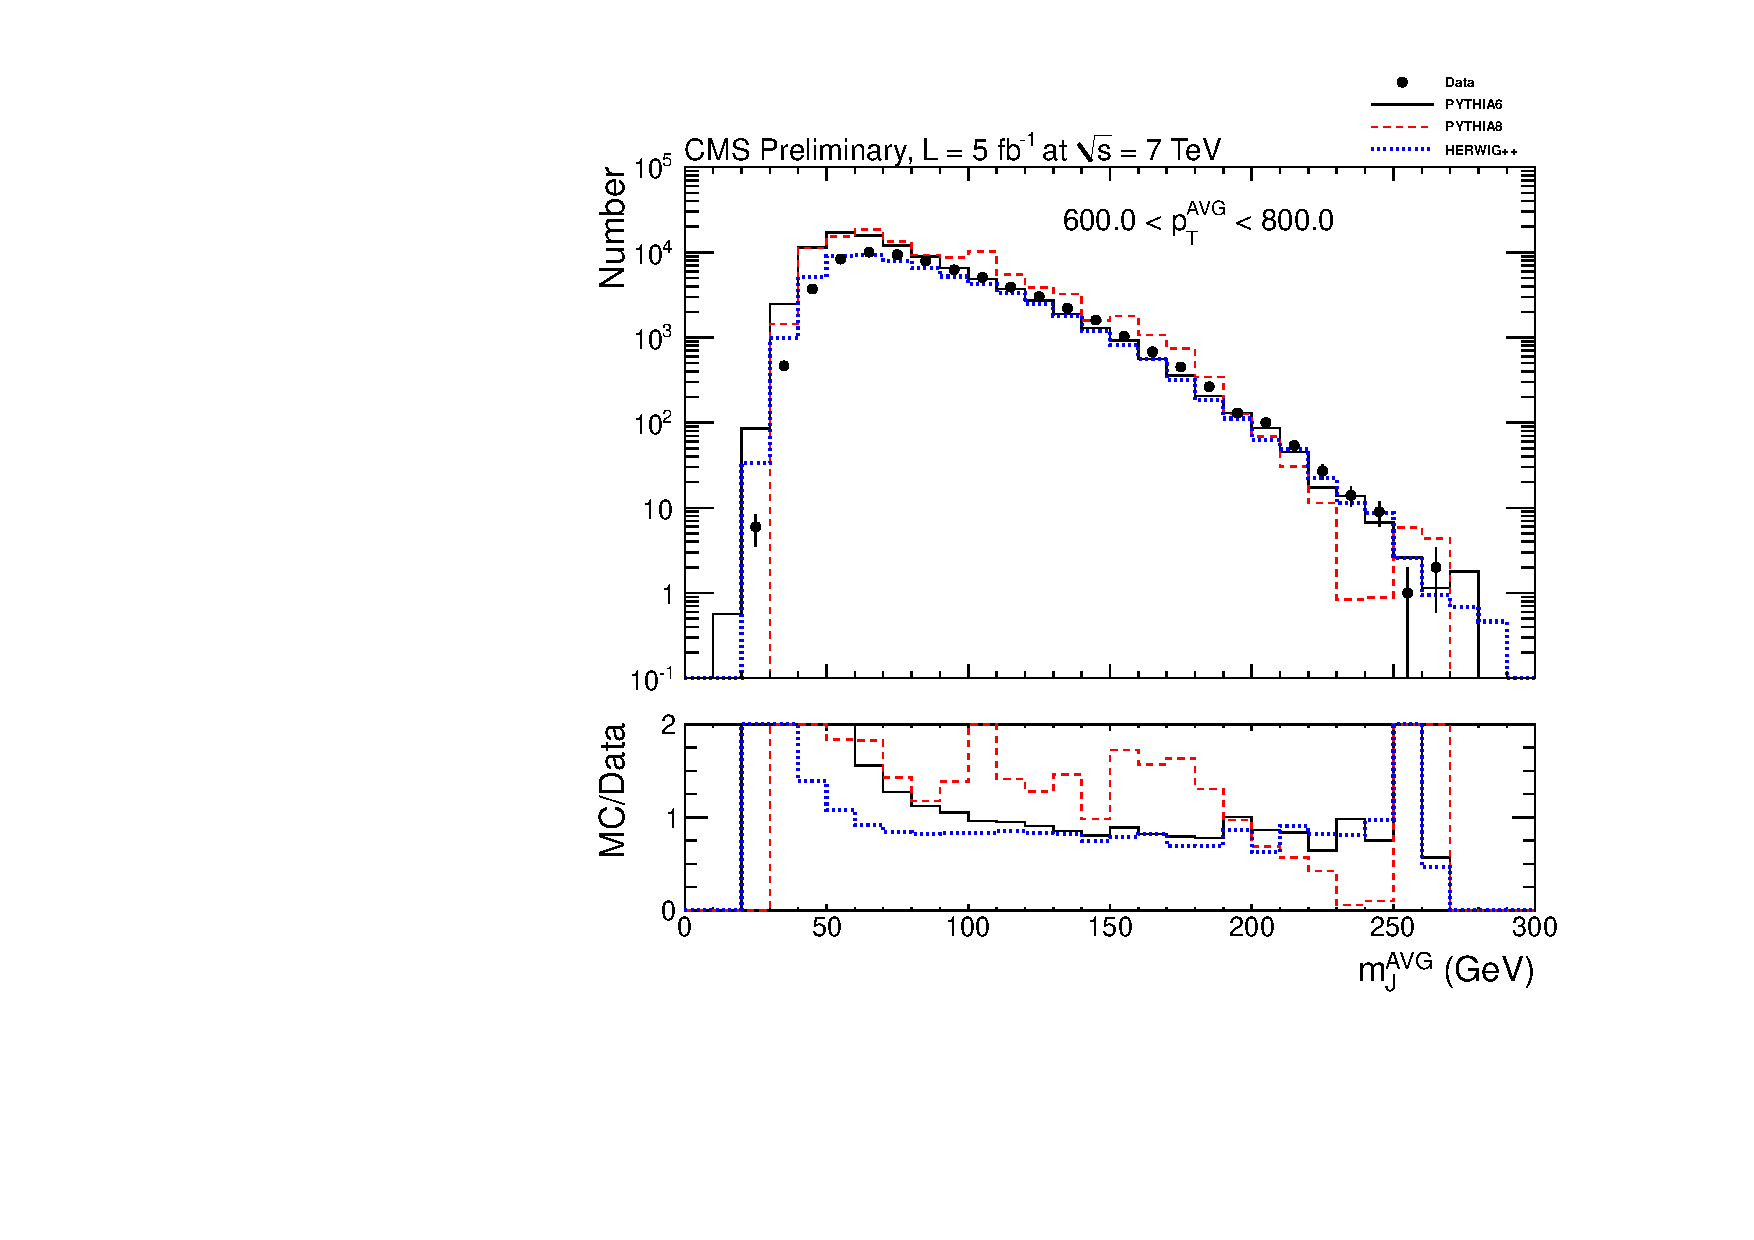
\includegraphics[width=0.95\textwidth]{figs/histAK7MjetVsPtAvg_rawDataMCComparisons_pt_8_Filtered}
\caption{Detector-level distributions of the jet mass for AK7 Filtered jets,
for $600.0 < \pt^{AVG} < 800.0$ \GeVc. The data are shown in black points.
The simulated distribution from \PYTHIA is shown in solid black, 
the from \PYTHIAEIGHT in dashed red, and from \HERWIG in dotted blue. 
The bottom frame shows the ratio of the simulated distribution
to the distribution from data. 
\label{figs:histAK7MjetVsPtAvg_rawDataMCComparisons_pt_8_Filtered}}
\end{figure}



\begin{figure}[htbp]
\centering
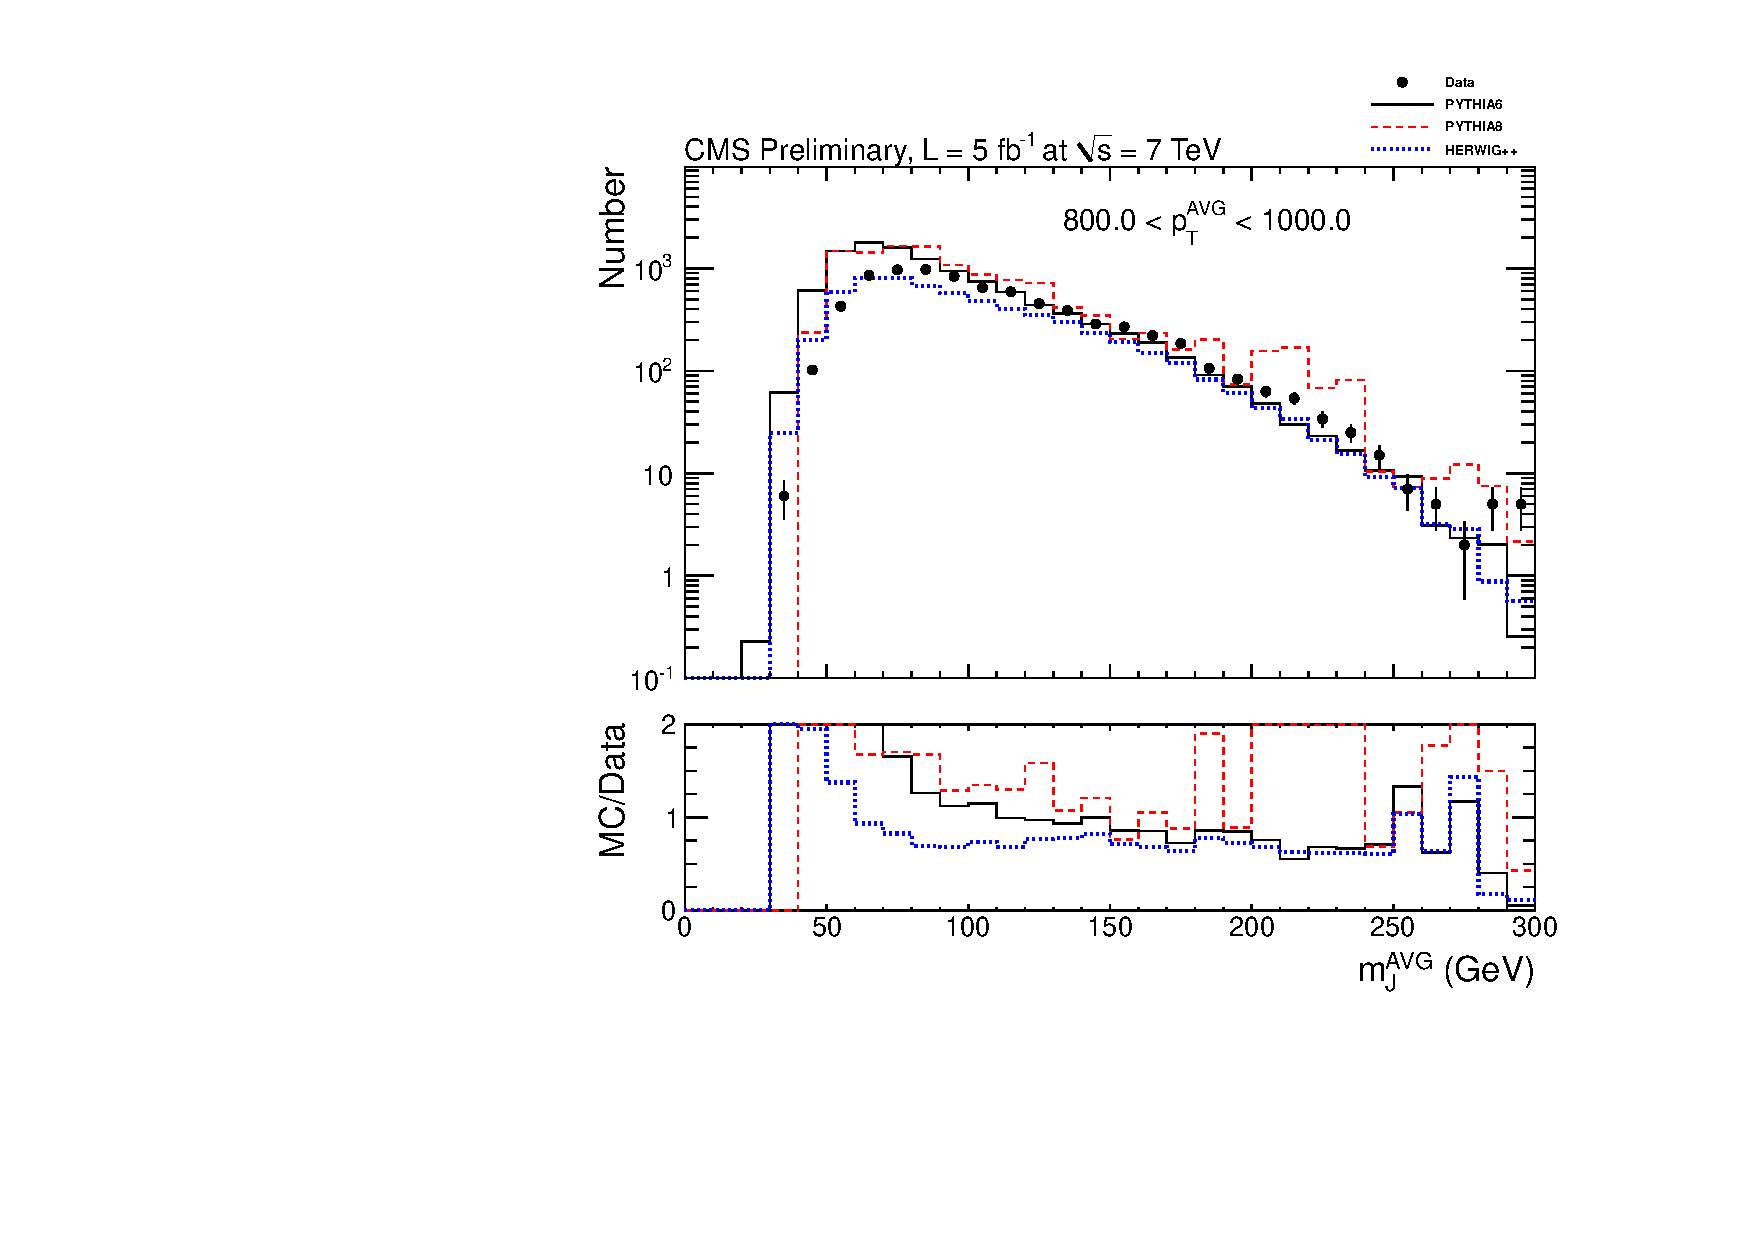
\includegraphics[width=0.95\textwidth]{figs/histAK7MjetVsPtAvg_rawDataMCComparisons_pt_9_Filtered}
\caption{Detector-level distributions of the jet mass for AK7 Filtered jets,
for $800.0 < \pt^{AVG} < 1000.0$ \GeVc. The data are shown in black points.
The simulated distribution from \PYTHIA is shown in solid black, 
the from \PYTHIAEIGHT in dashed red, and from \HERWIG in dotted blue. 
The bottom frame shows the ratio of the simulated distribution
to the distribution from data. 
\label{figs:histAK7MjetVsPtAvg_rawDataMCComparisons_pt_9_Filtered}}
\end{figure}



\begin{figure}[htbp]
\centering
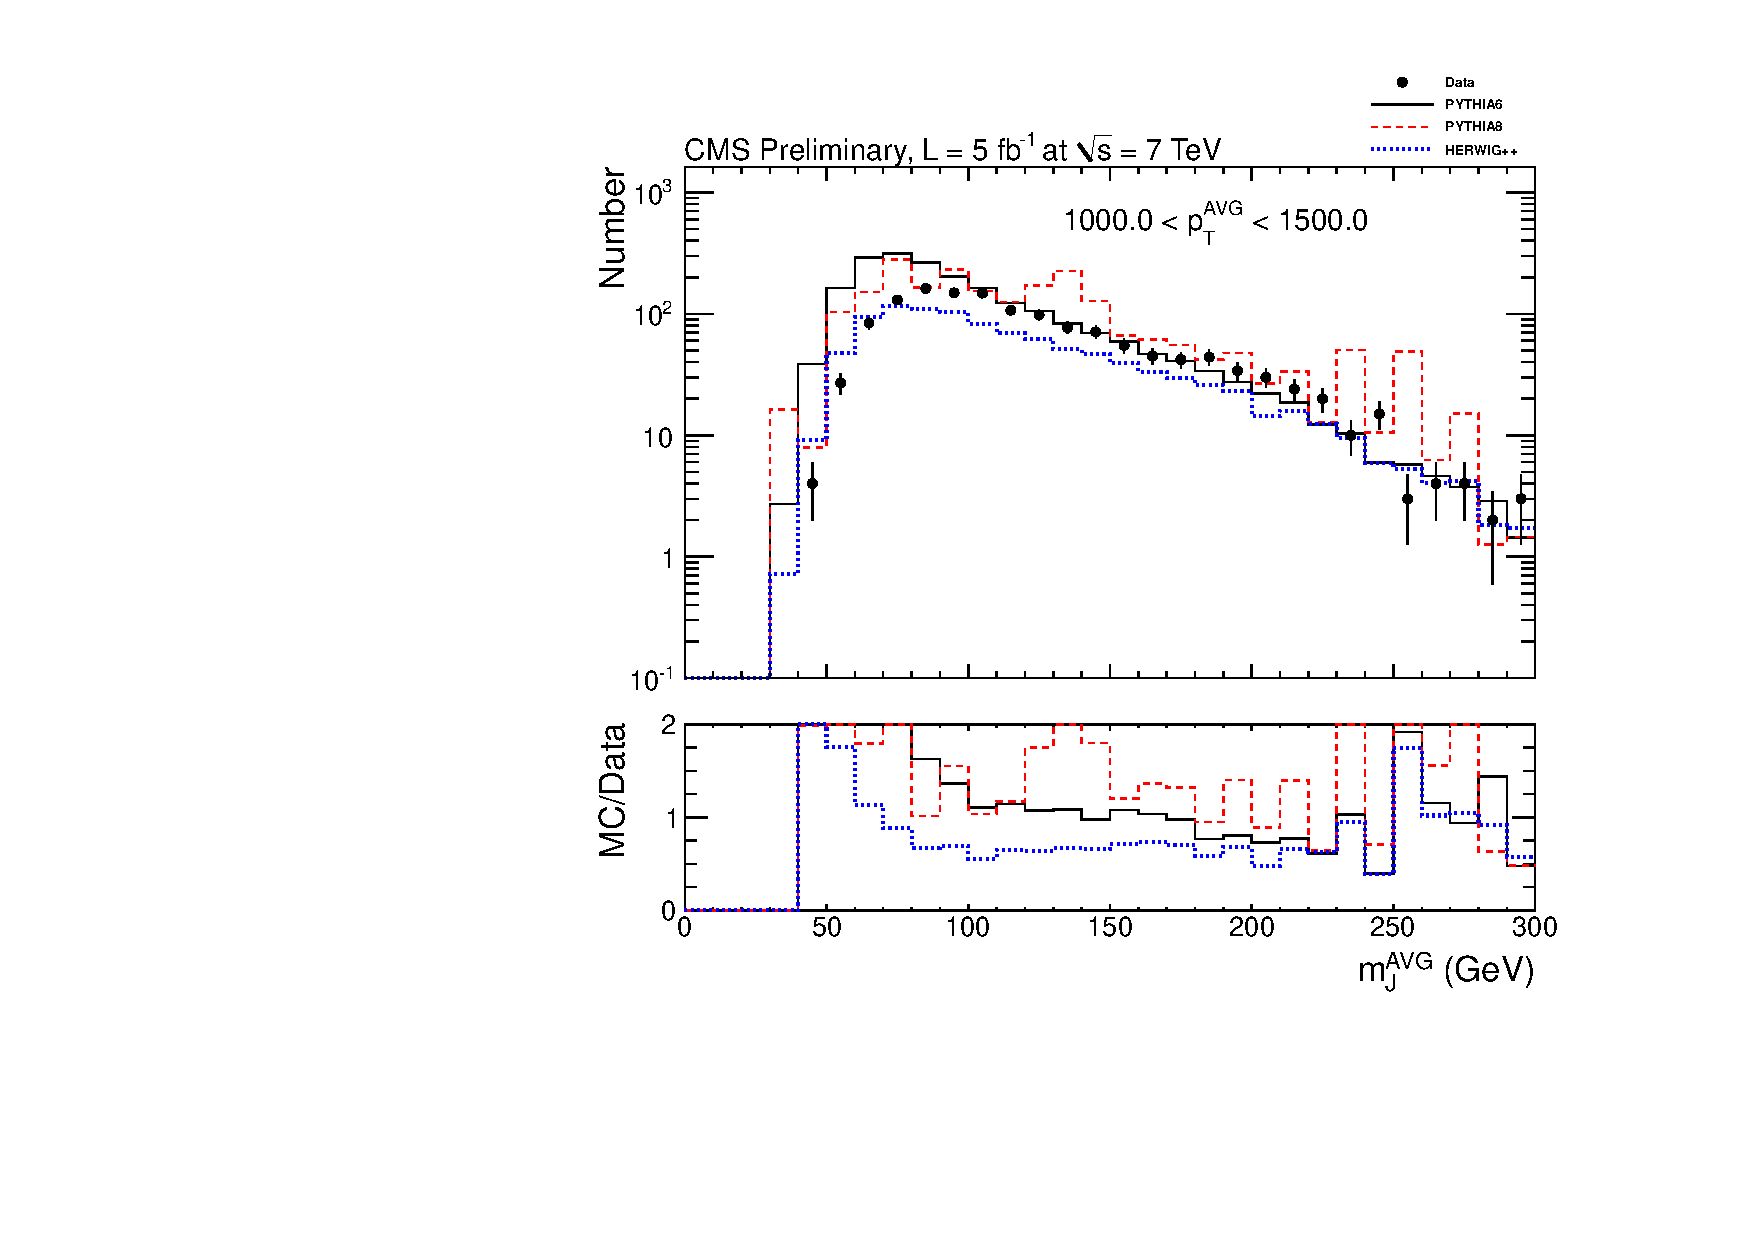
\includegraphics[width=0.95\textwidth]{figs/histAK7MjetVsPtAvg_rawDataMCComparisons_pt_10_Filtered}
\caption{Detector-level distributions of the jet mass for AK7 Filtered jets,
for $1000.0 < \pt^{AVG} < 1500.0$ \GeVc. The data are shown in black points.
The simulated distribution from \PYTHIA is shown in solid black, 
the from \PYTHIAEIGHT in dashed red, and from \HERWIG in dotted blue. 
The bottom frame shows the ratio of the simulated distribution
to the distribution from data. 
\label{figs:histAK7MjetVsPtAvg_rawDataMCComparisons_pt_10_Filtered}}
\end{figure}

\fi

\clearpage


\ifnpas

\begin{figure}[htbp]
\centering
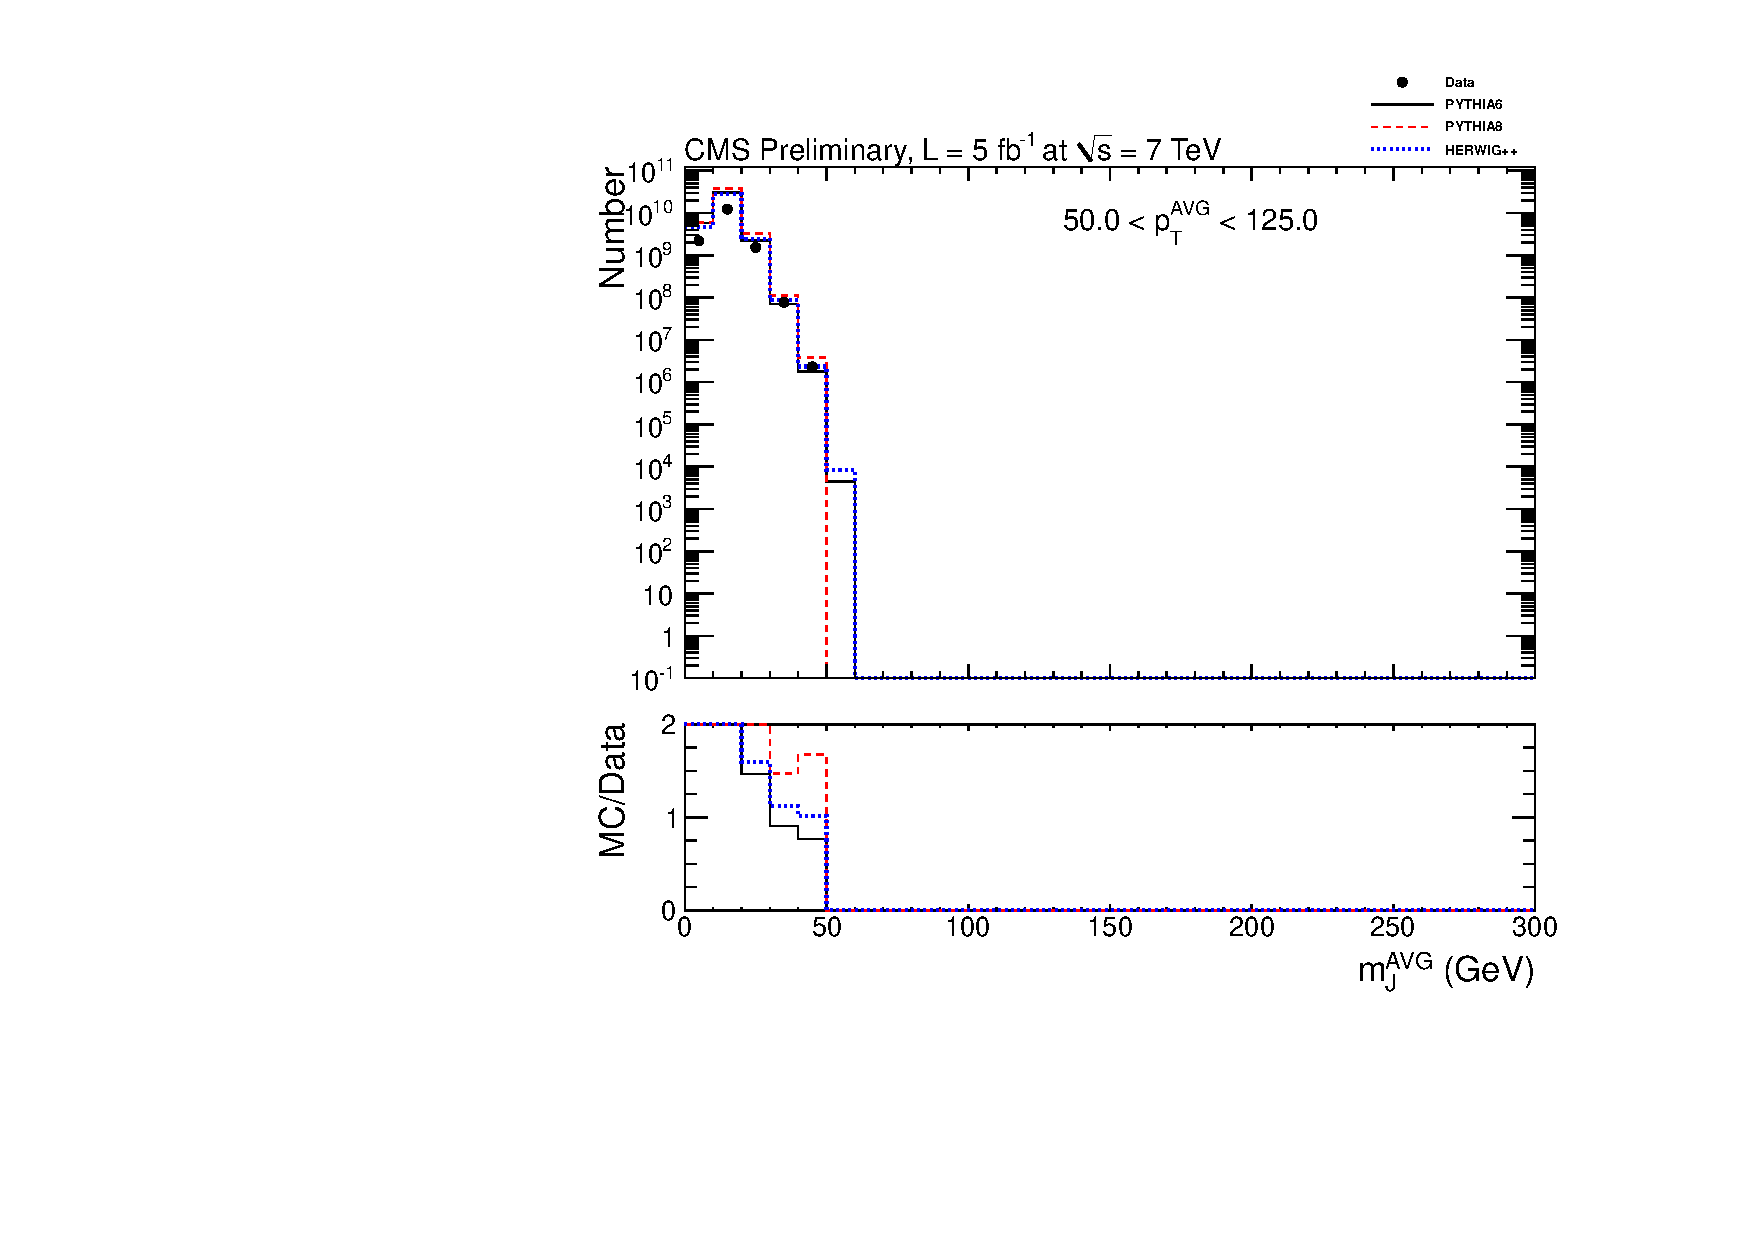
\includegraphics[width=0.95\textwidth]{figs/histAK7MjetVsPtAvg_rawDataMCComparisons_pt_1_Trimmed}
\caption{Detector-level distributions of the jet mass for AK7 Trimmed jets,
for $50.0 < \pt^{AVG} < 125.0$ \GeVc. The data are shown in black points.
The simulated distribution from \PYTHIA is shown in solid black, 
the from \PYTHIAEIGHT in dashed red, and from \HERWIG in dotted blue. 
The bottom frame shows the ratio of the simulated distribution
to the distribution from data. 
\label{figs:histAK7MjetVsPtAvg_rawDataMCComparisons_pt_1_Trimmed}}
\end{figure}

\fi

\begin{figure}[htbp]
\centering
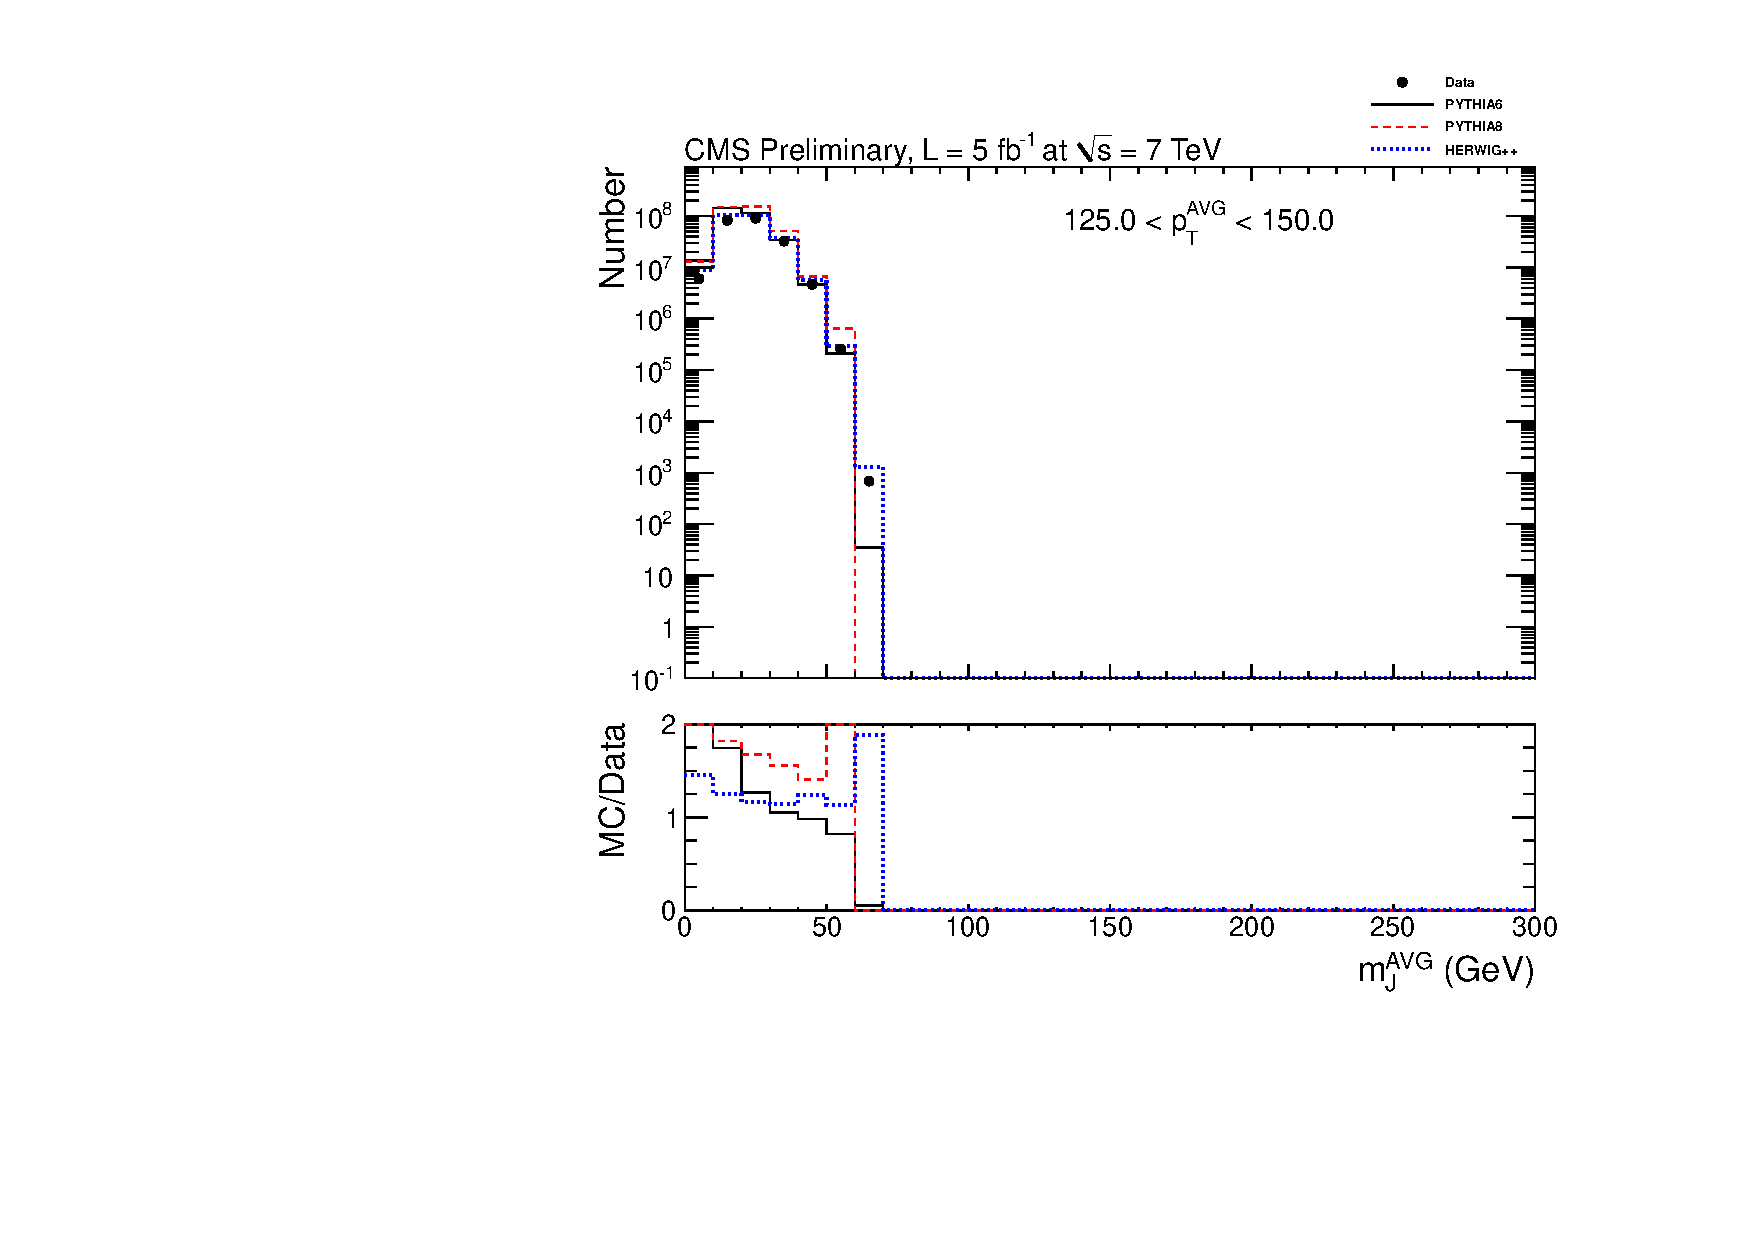
\includegraphics[width=0.49\textwidth]{figs/histAK7MjetVsPtAvg_rawDataMCComparisons_pt_2_Trimmed}
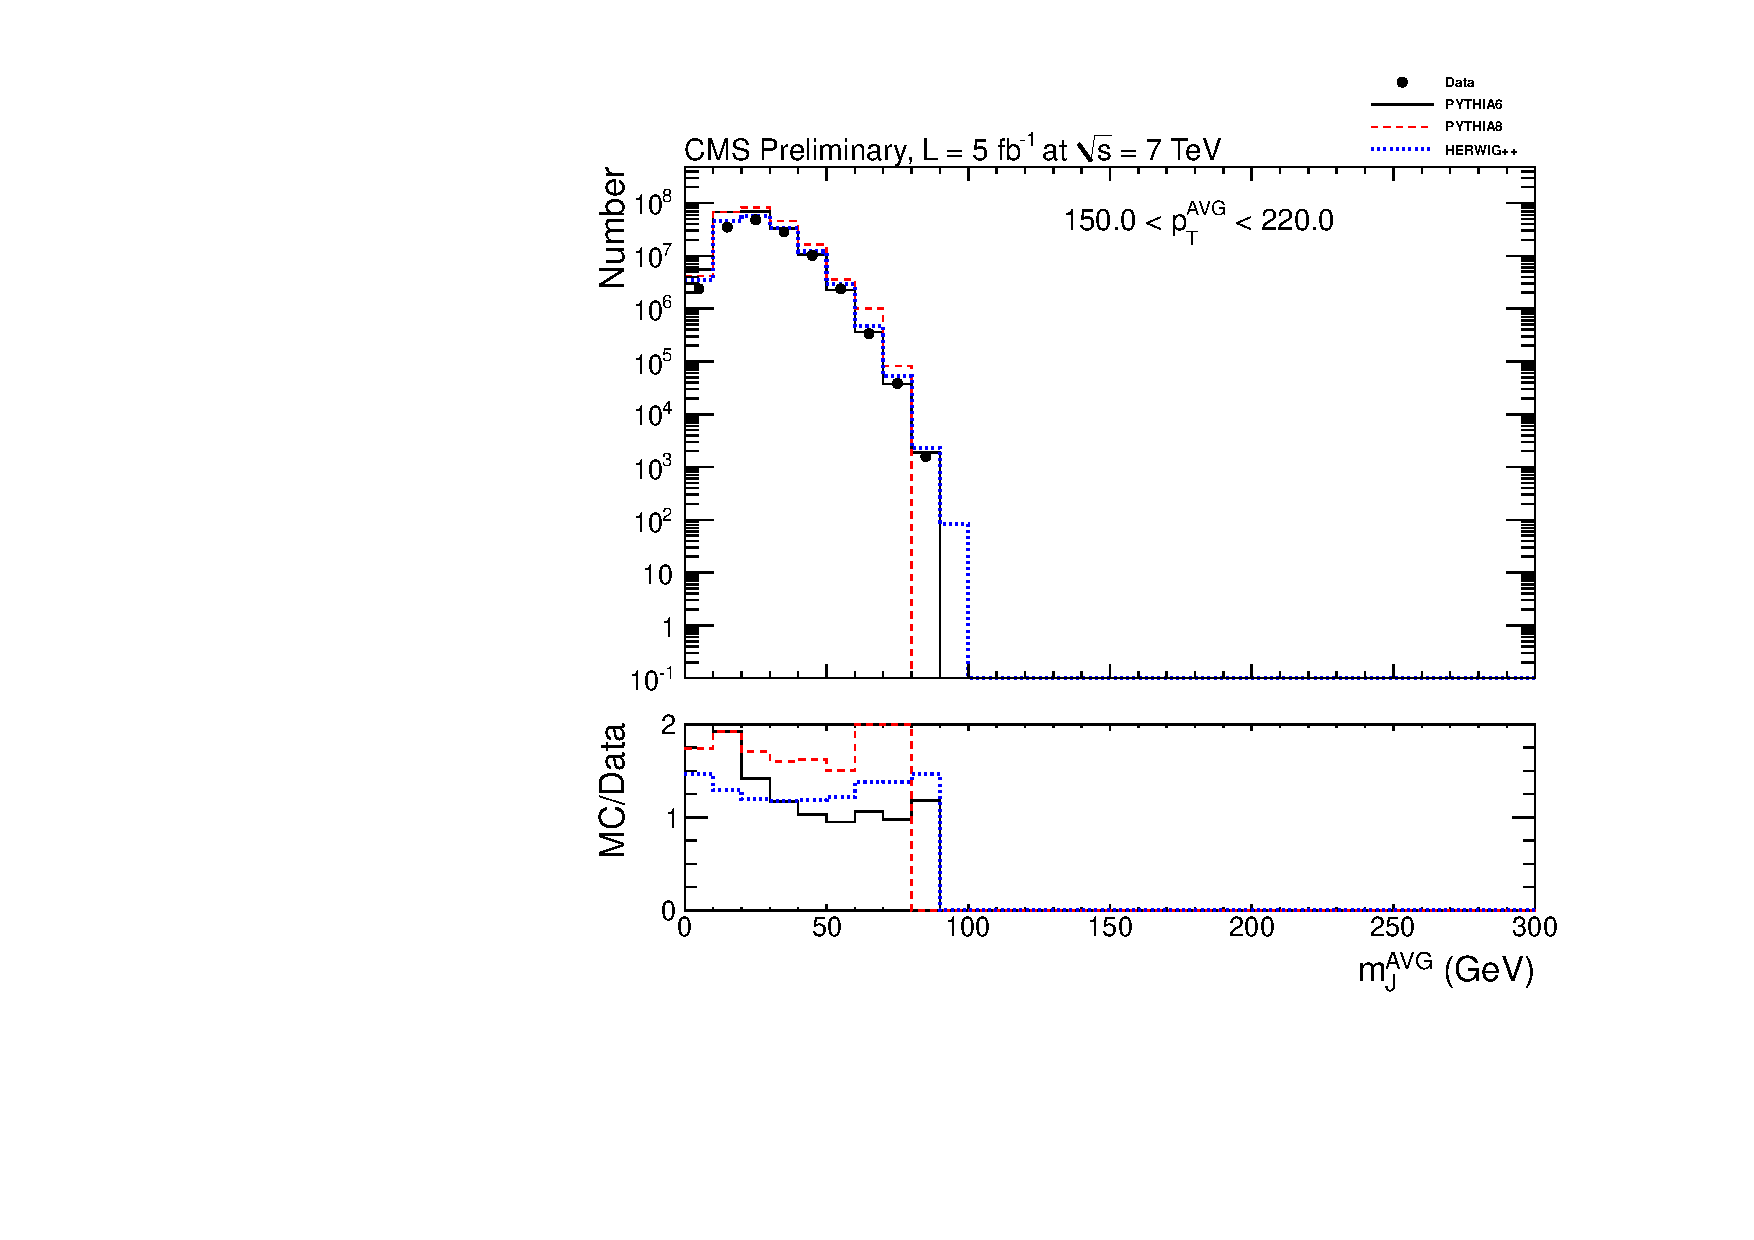
\includegraphics[width=0.49\textwidth]{figs/histAK7MjetVsPtAvg_rawDataMCComparisons_pt_3_Trimmed}
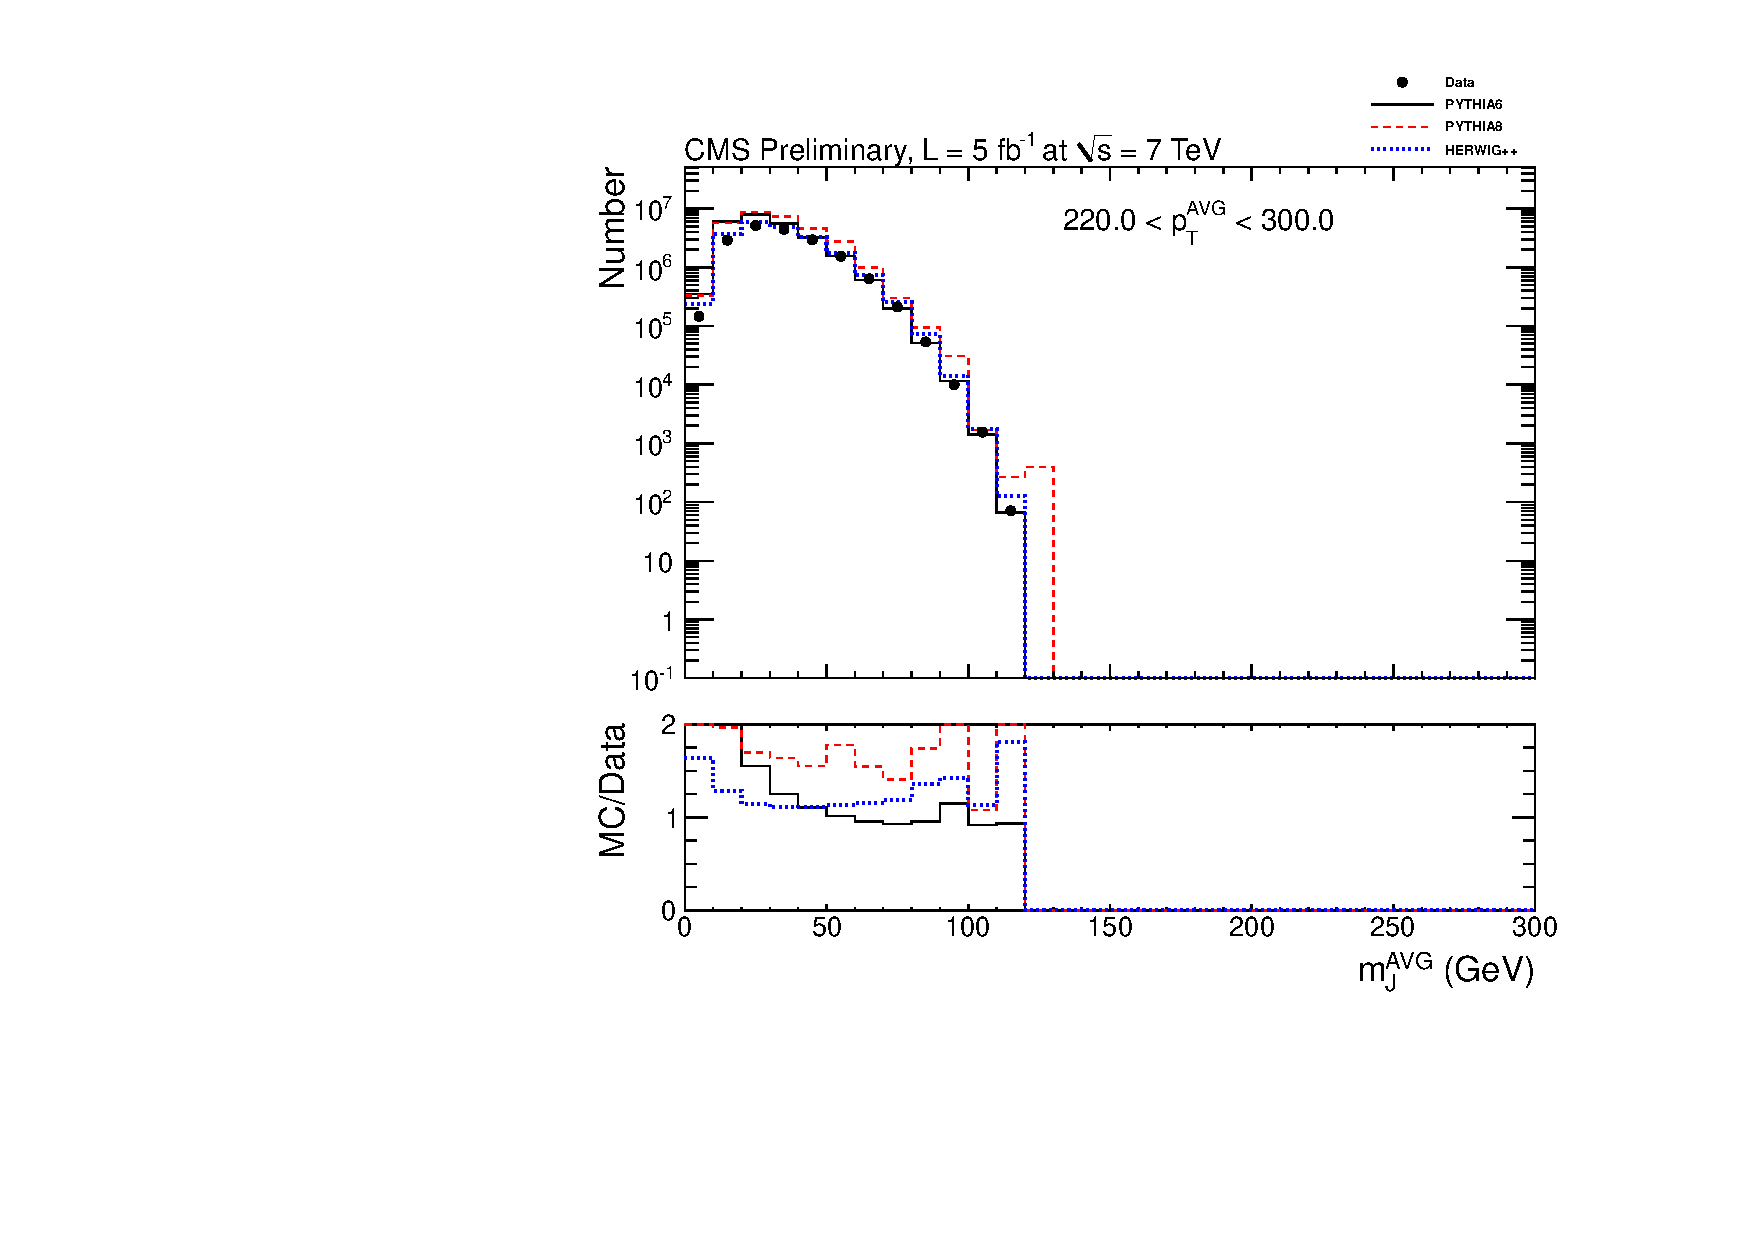
\includegraphics[width=0.49\textwidth]{figs/histAK7MjetVsPtAvg_rawDataMCComparisons_pt_4_Trimmed}
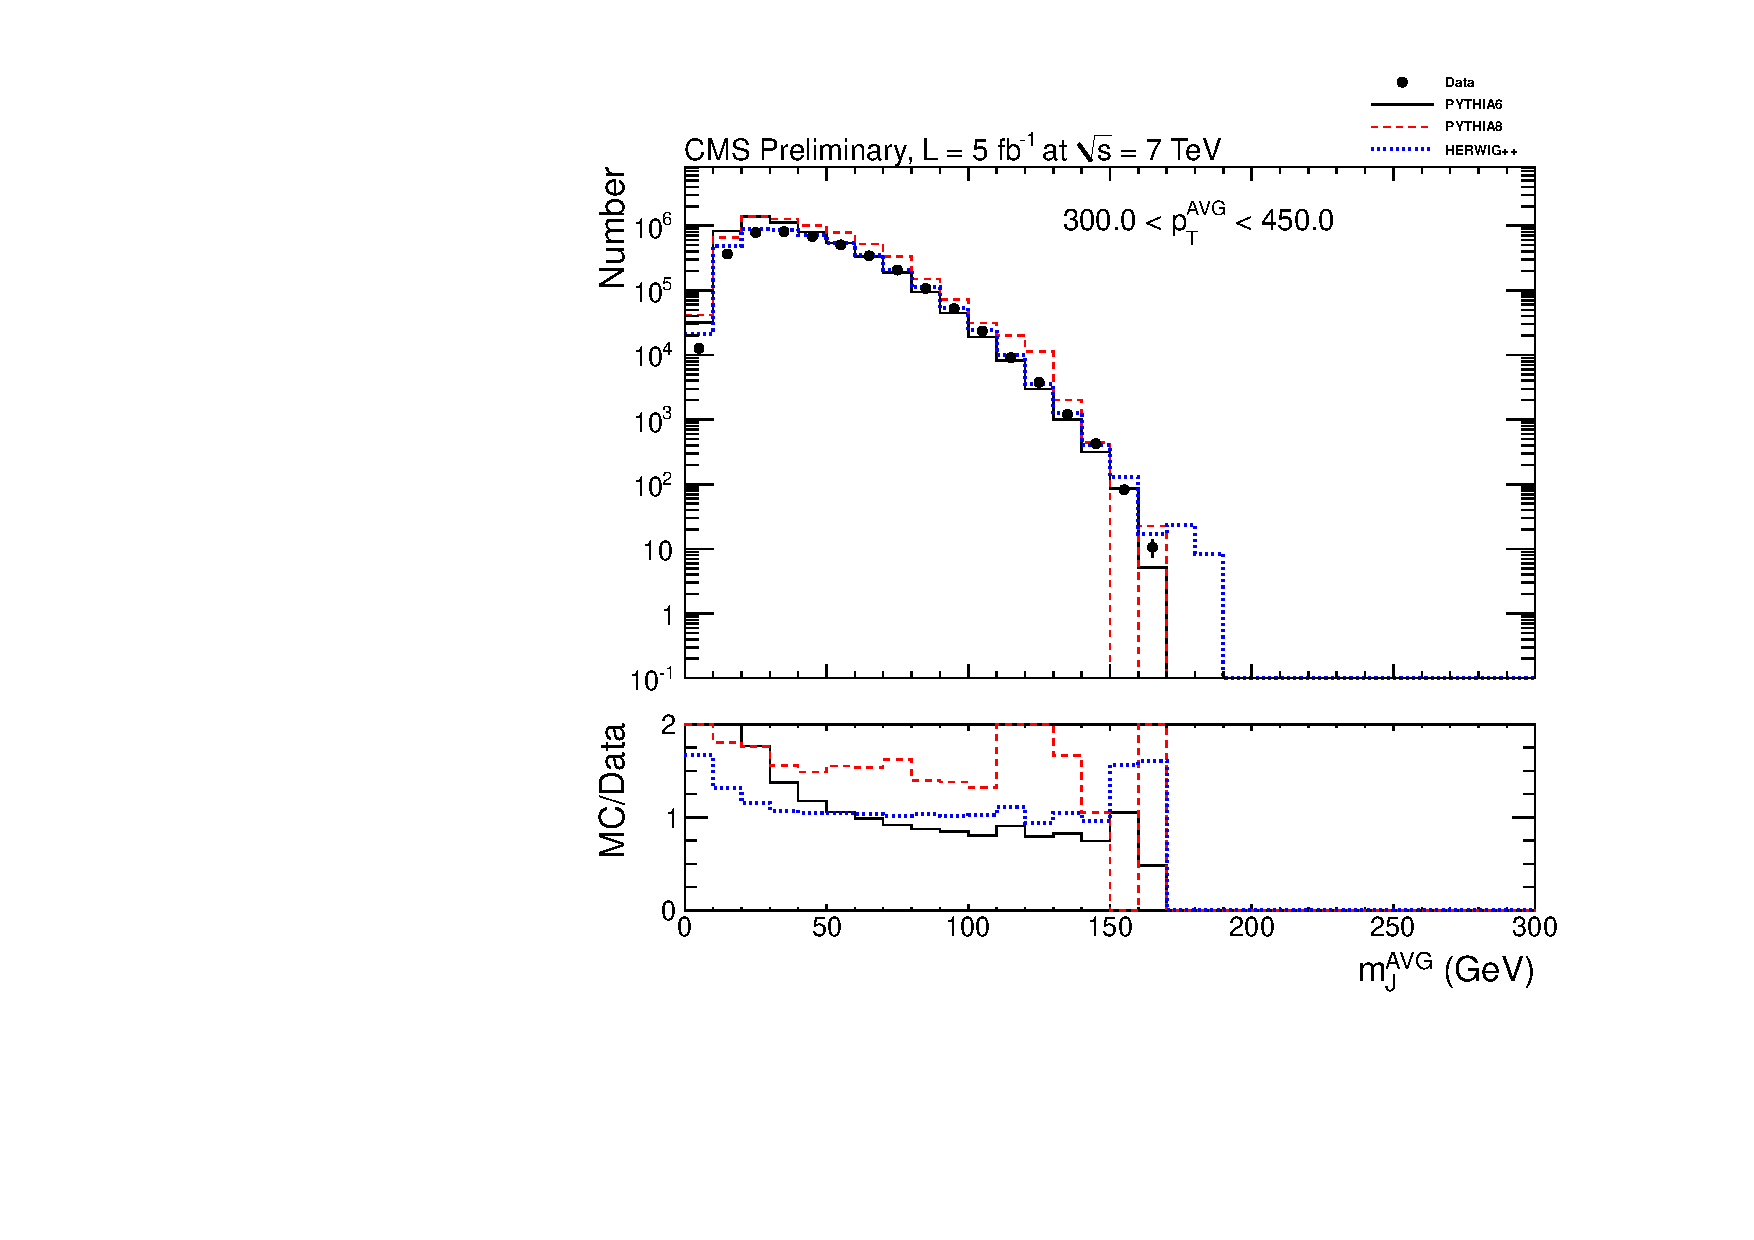
\includegraphics[width=0.49\textwidth]{figs/histAK7MjetVsPtAvg_rawDataMCComparisons_pt_5_Trimmed}
\caption{Detector-level distributions of the jet mass for AK7 Trimmed jets,
for several $\pt^{AVG}$ bins. The data are shown in black points.
%for $125.0 < \pt^{AVG} < 150.0$ \GeVc. The data are shown in black points.
The simulated distribution from \PYTHIA is shown in solid black, 
the from \PYTHIAEIGHT in dashed red, and from \HERWIG in dotted blue. 
The bottom frame shows the ratio of the simulated distribution
to the distribution from data. 
\label{figs:histAK7MjetVsPtAvg_rawDataMCComparisons_pt_2_Trimmed}}
\end{figure}

%%%%%%%%
\ifnpas


\begin{figure}[htbp]
\centering
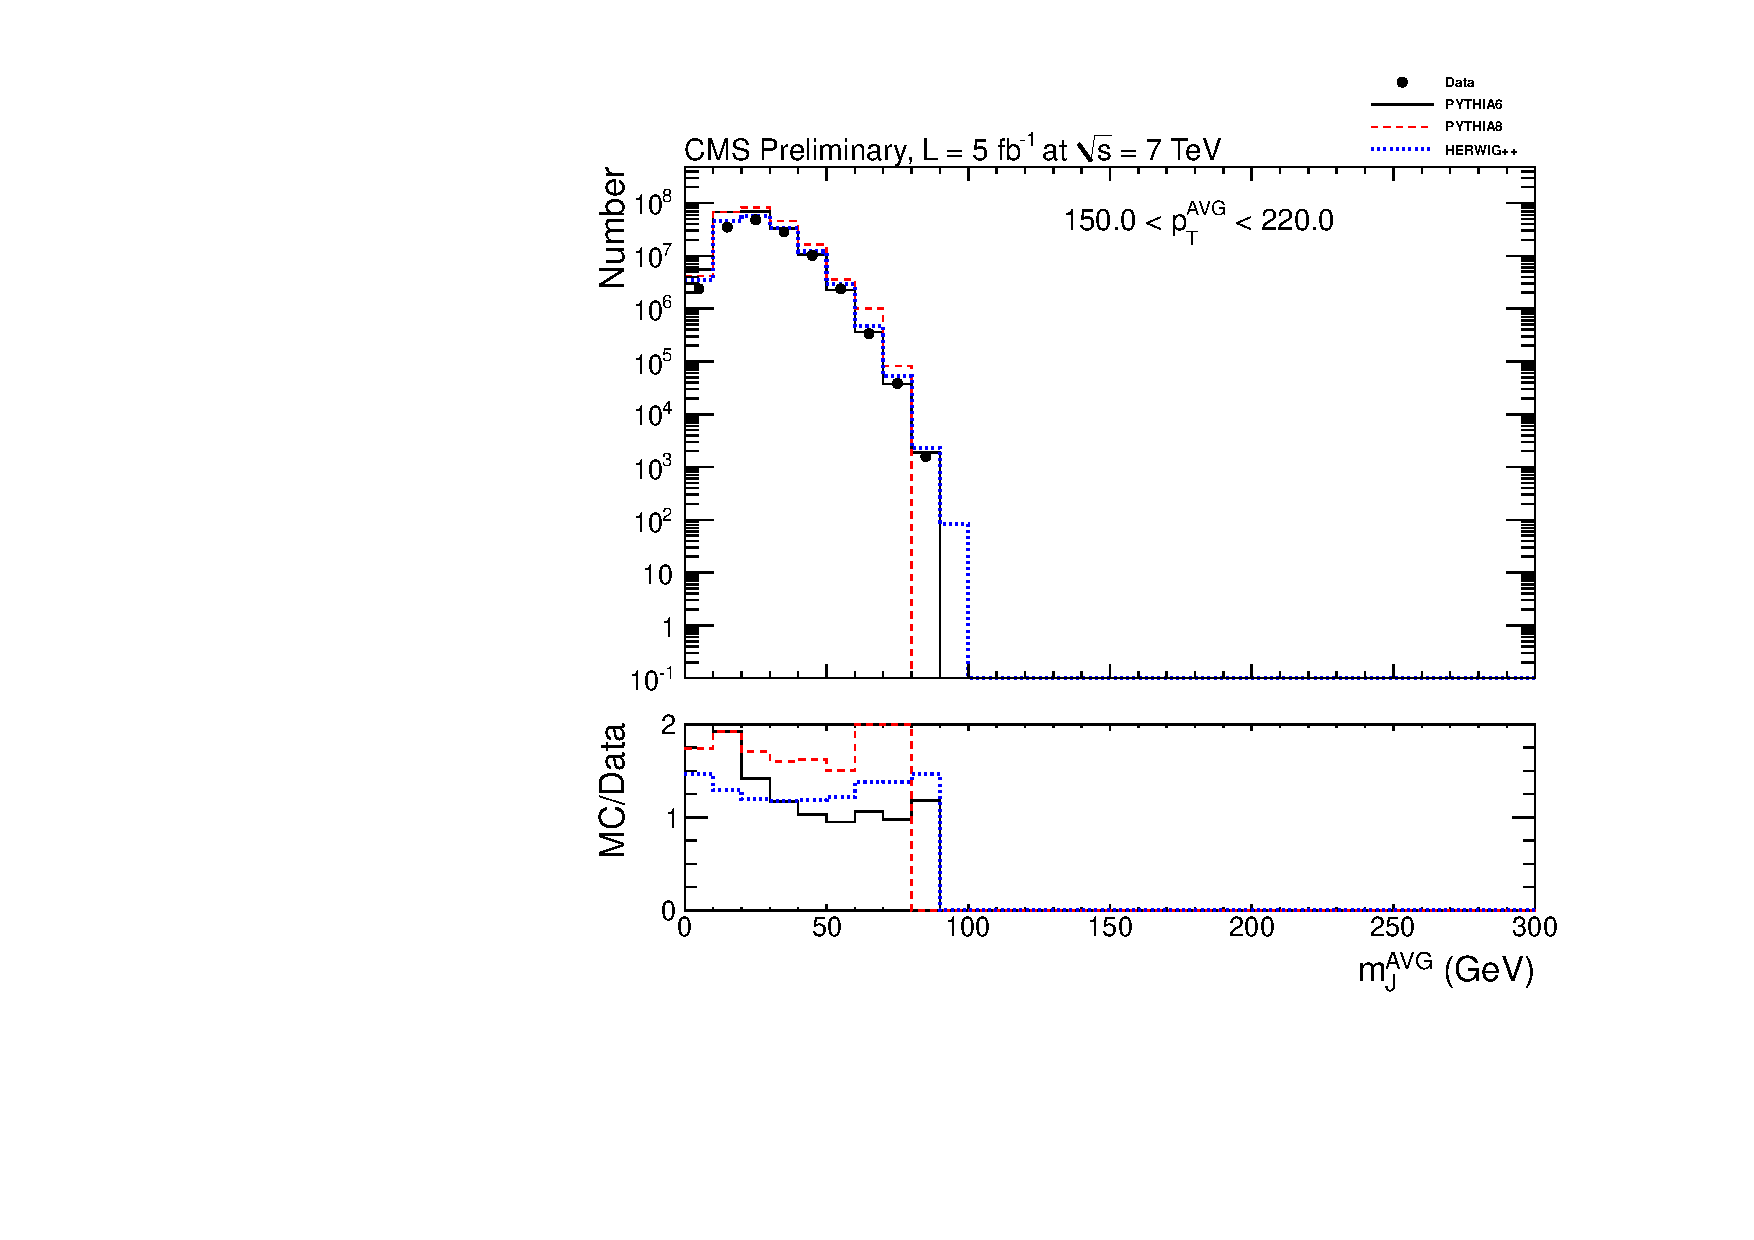
\includegraphics[width=0.95\textwidth]{figs/histAK7MjetVsPtAvg_rawDataMCComparisons_pt_3_Trimmed}
\caption{Detector-level distributions of the jet mass for AK7 Trimmed jets,
for $150.0 < \pt^{AVG} < 220.0$ \GeVc. The data are shown in black points.
The simulated distribution from \PYTHIA is shown in solid black, 
the from \PYTHIAEIGHT in dashed red, and from \HERWIG in dotted blue. 
The bottom frame shows the ratio of the simulated distribution
to the distribution from data. 
\label{figs:histAK7MjetVsPtAvg_rawDataMCComparisons_pt_3_Trimmed}}
\end{figure}



\begin{figure}[htbp]
\centering
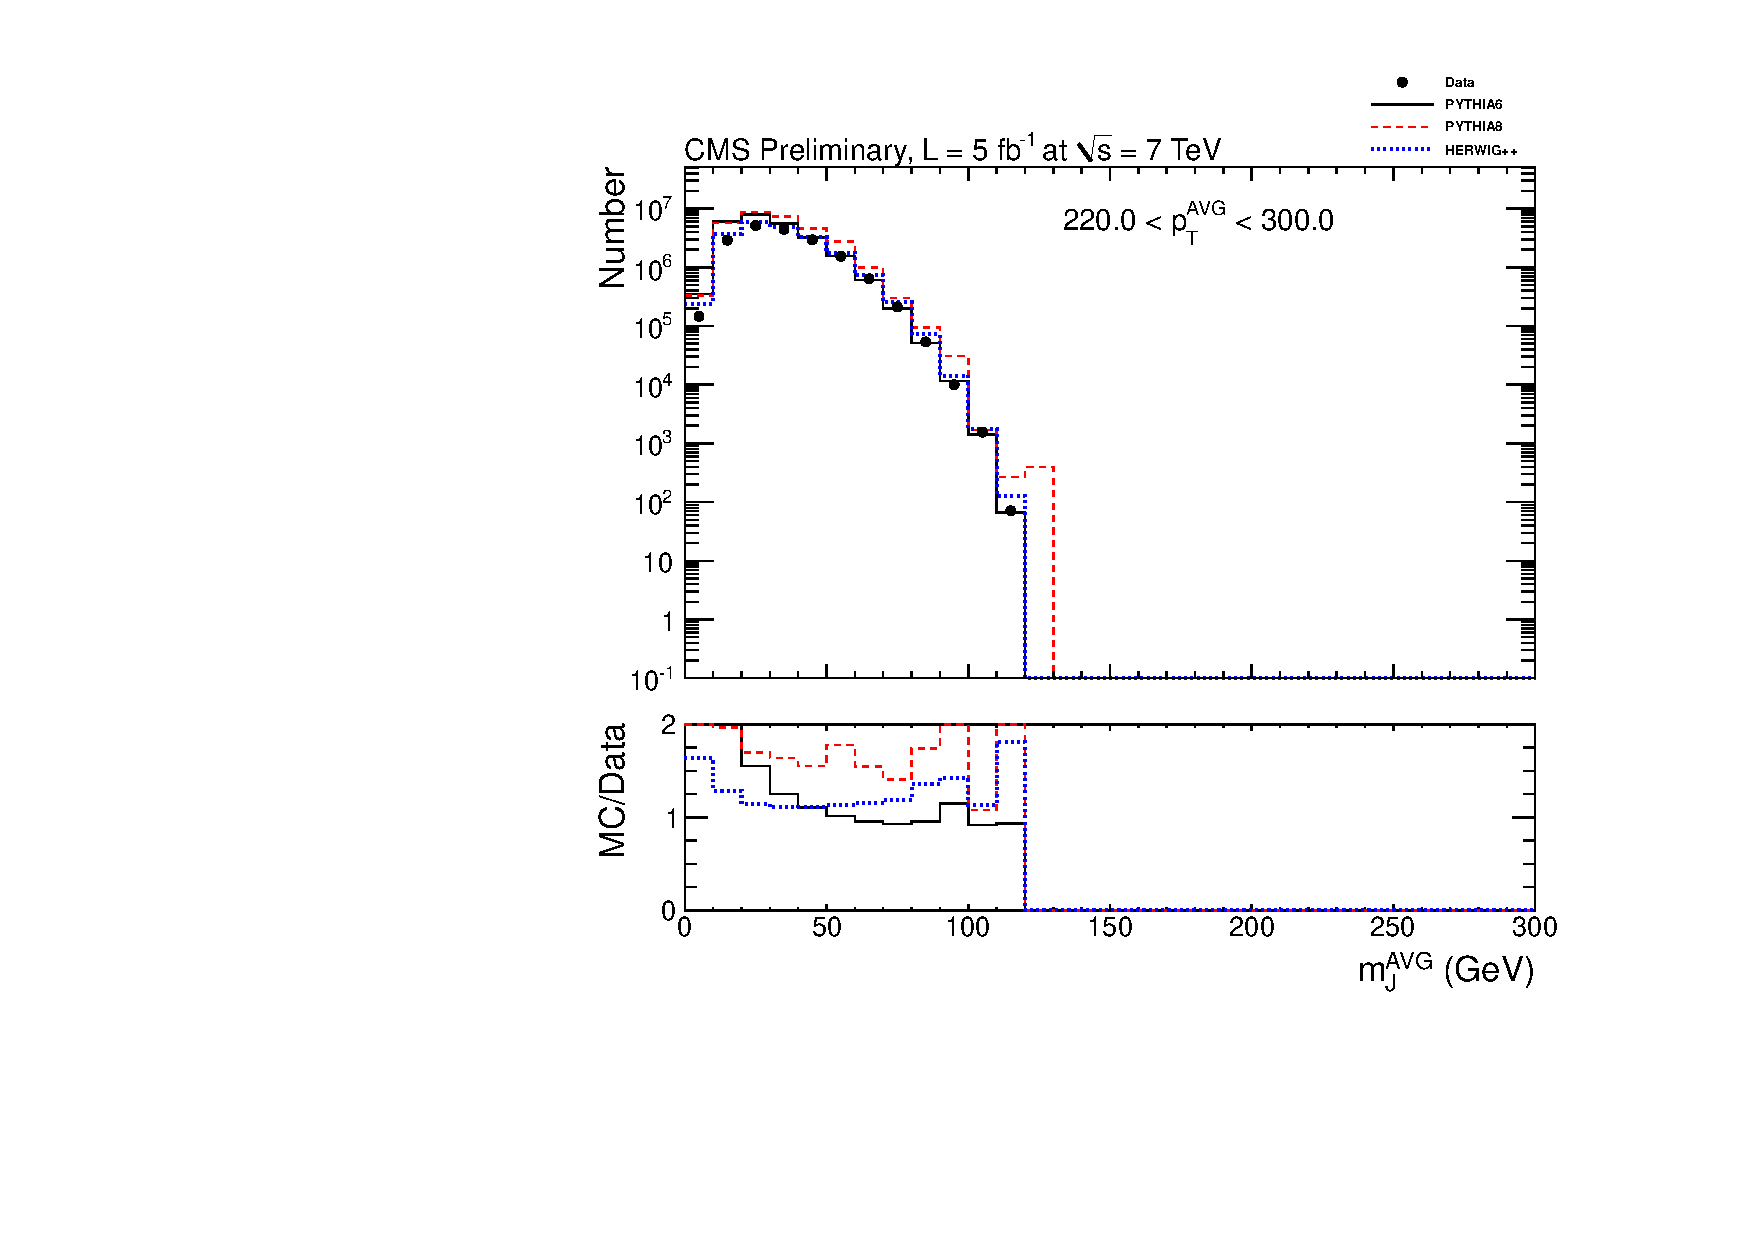
\includegraphics[width=0.95\textwidth]{figs/histAK7MjetVsPtAvg_rawDataMCComparisons_pt_4_Trimmed}
\caption{Detector-level distributions of the jet mass for AK7 Trimmed jets,
for $220.0 < \pt^{AVG} < 300.0$ \GeVc. The data are shown in black points.
The simulated distribution from \PYTHIA is shown in solid black, 
the from \PYTHIAEIGHT in dashed red, and from \HERWIG in dotted blue. 
The bottom frame shows the ratio of the simulated distribution
to the distribution from data. 
\label{figs:histAK7MjetVsPtAvg_rawDataMCComparisons_pt_4_Trimmed}}
\end{figure}



\begin{figure}[htbp]
\centering
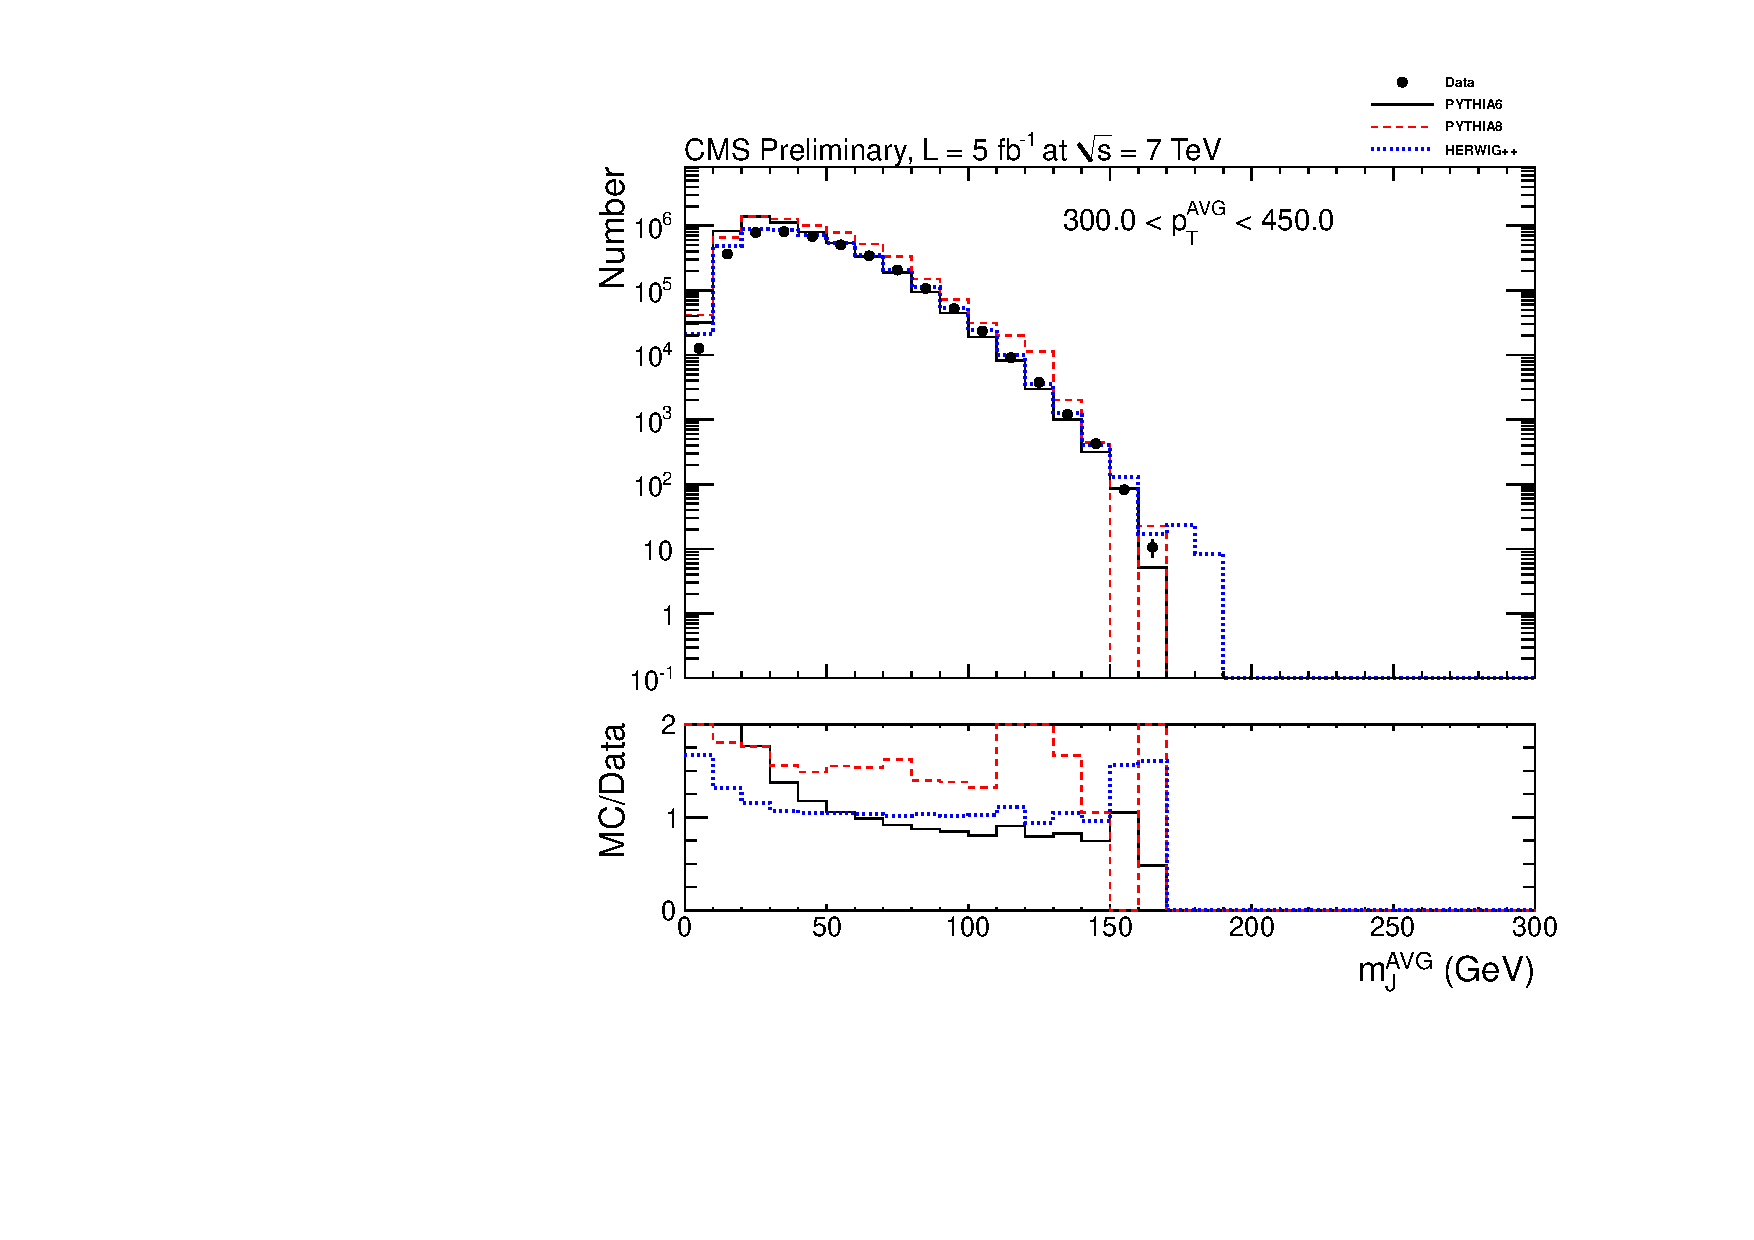
\includegraphics[width=0.95\textwidth]{figs/histAK7MjetVsPtAvg_rawDataMCComparisons_pt_5_Trimmed}
\caption{Detector-level distributions of the jet mass for AK7 Trimmed jets,
for $300.0 < \pt^{AVG} < 450.0$ \GeVc. The data are shown in black points.
The simulated distribution from \PYTHIA is shown in solid black, 
the from \PYTHIAEIGHT in dashed red, and from \HERWIG in dotted blue. 
The bottom frame shows the ratio of the simulated distribution
to the distribution from data. 
\label{figs:histAK7MjetVsPtAvg_rawDataMCComparisons_pt_5_Trimmed}}
\end{figure}

\fi
%%%%%%%%%%%%


\ifnpas

\begin{figure}[htbp]
\centering
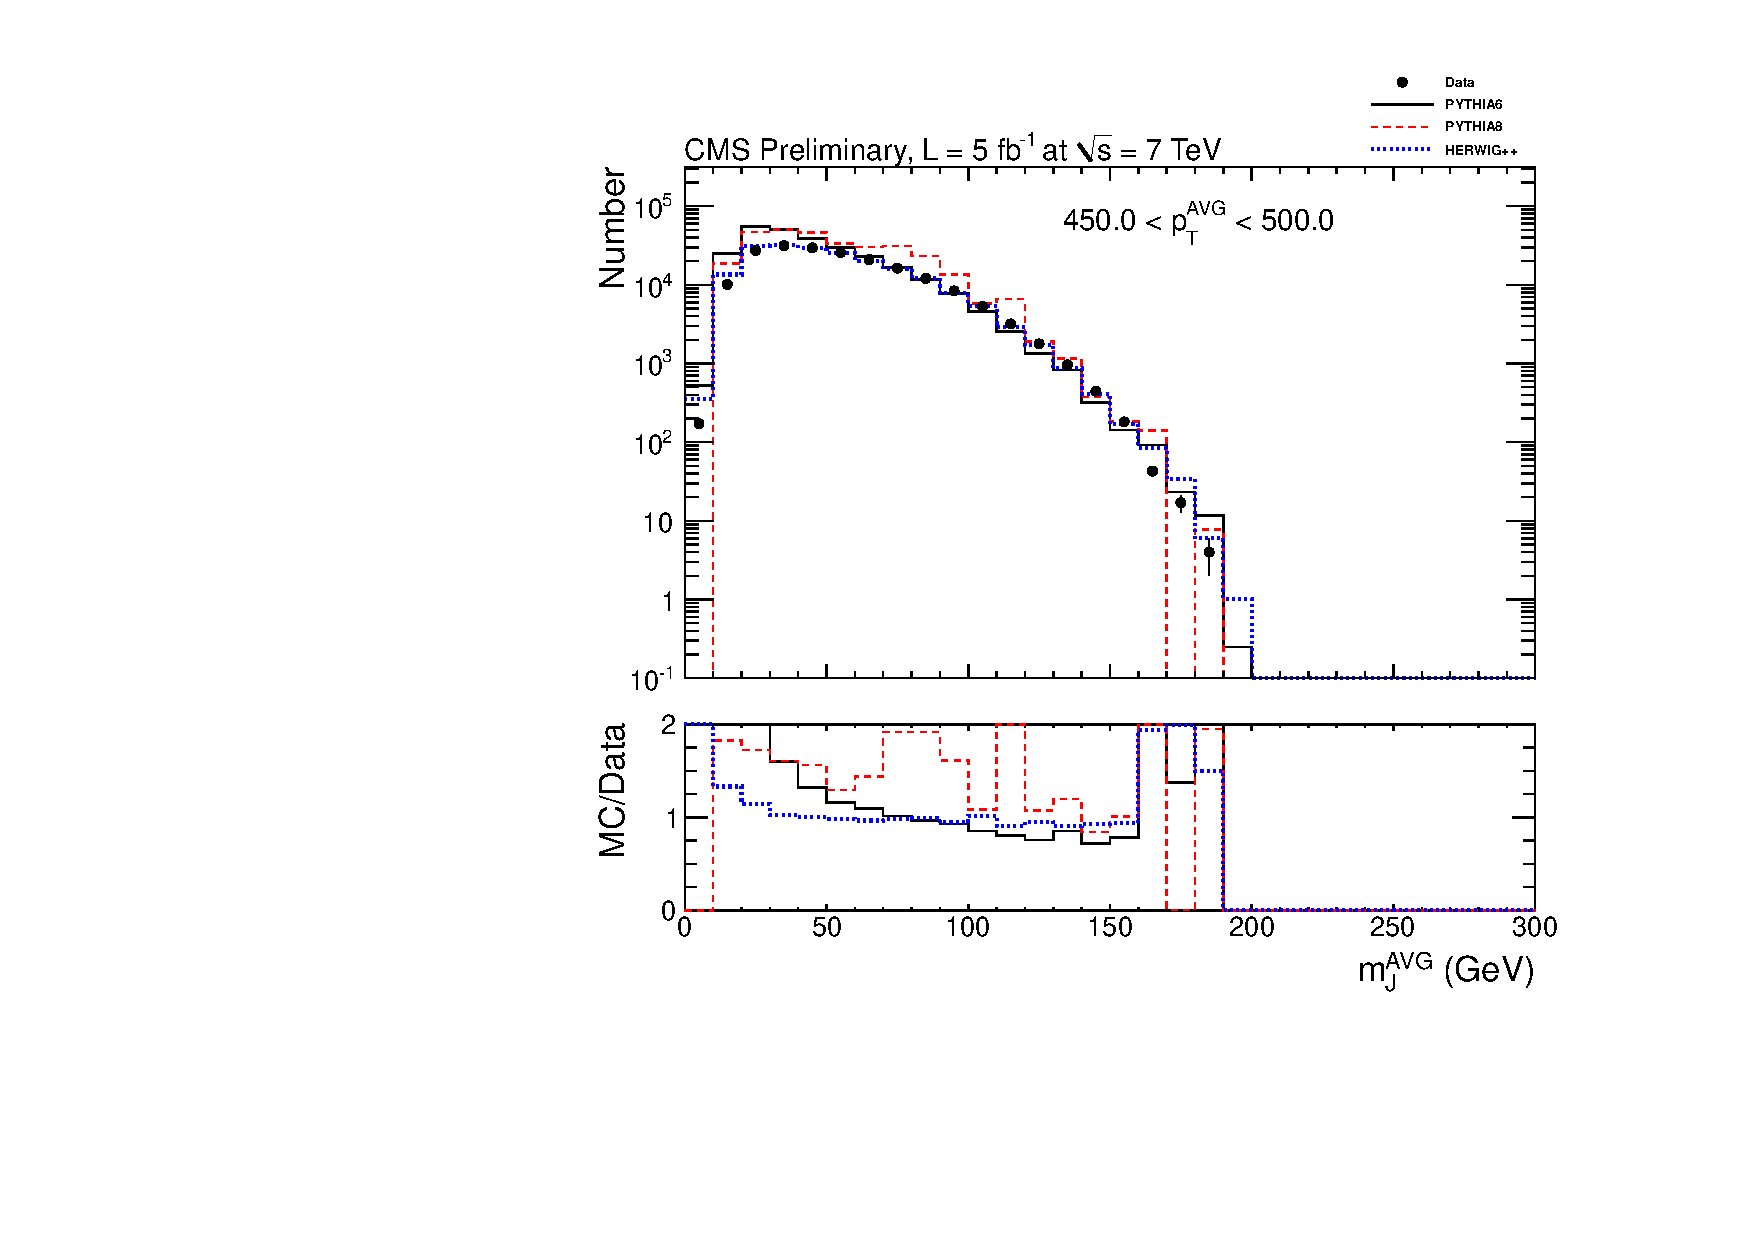
\includegraphics[width=0.95\textwidth]{figs/histAK7MjetVsPtAvg_rawDataMCComparisons_pt_6_Trimmed}
\caption{Detector-level distributions of the jet mass for AK7 Trimmed jets,
for $450.0 < \pt^{AVG} < 500.0$ \GeVc. The data are shown in black points.
The simulated distribution from \PYTHIA is shown in solid black, 
the from \PYTHIAEIGHT in dashed red, and from \HERWIG in dotted blue. 
The bottom frame shows the ratio of the simulated distribution
to the distribution from data. 
\label{figs:histAK7MjetVsPtAvg_rawDataMCComparisons_pt_6_Trimmed}}
\end{figure}



\begin{figure}[htbp]
\centering
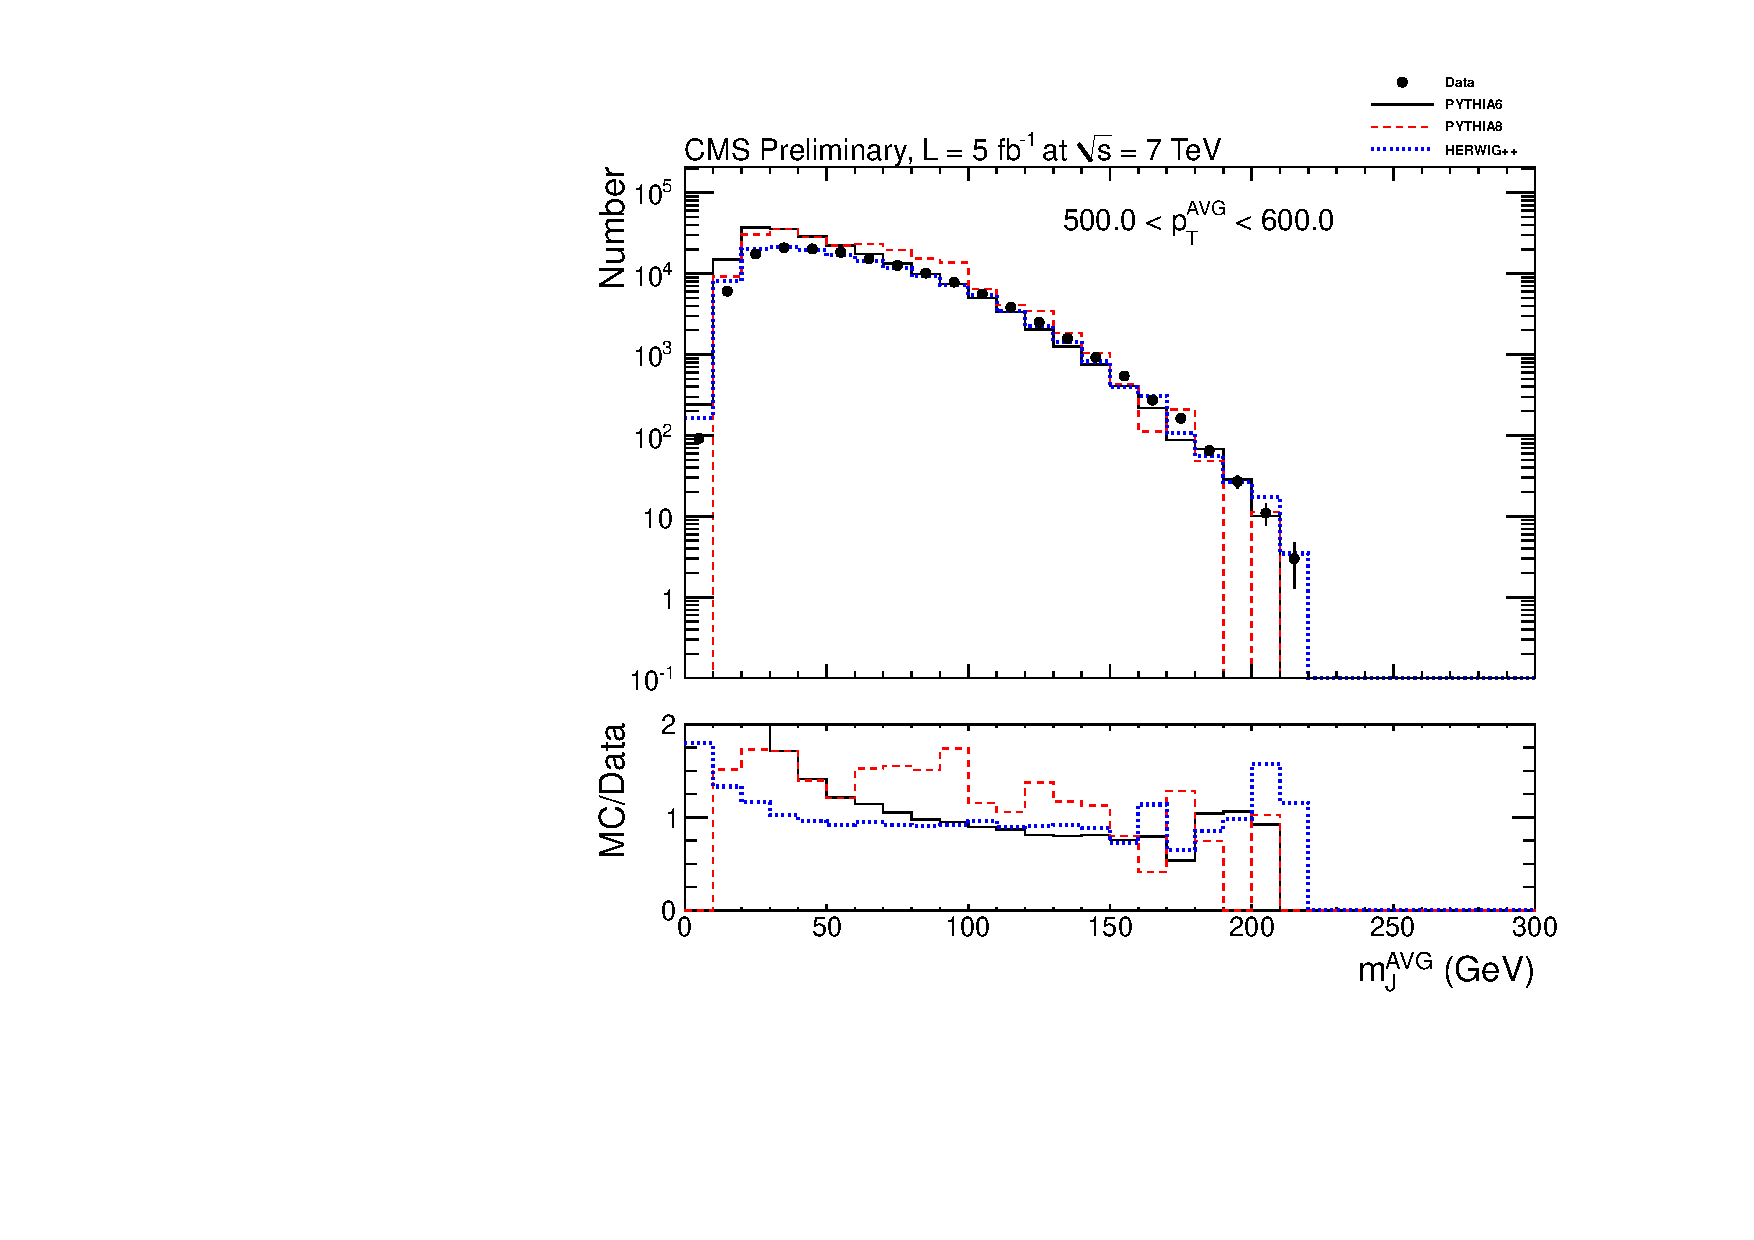
\includegraphics[width=0.95\textwidth]{figs/histAK7MjetVsPtAvg_rawDataMCComparisons_pt_7_Trimmed}
\caption{Detector-level distributions of the jet mass for AK7 Trimmed jets,
for $500.0 < \pt^{AVG} < 600.0$ \GeVc. The data are shown in black points.
The simulated distribution from \PYTHIA is shown in solid black, 
the from \PYTHIAEIGHT in dashed red, and from \HERWIG in dotted blue. 
The bottom frame shows the ratio of the simulated distribution
to the distribution from data. 
\label{figs:histAK7MjetVsPtAvg_rawDataMCComparisons_pt_7_Trimmed}}
\end{figure}



\begin{figure}[htbp]
\centering
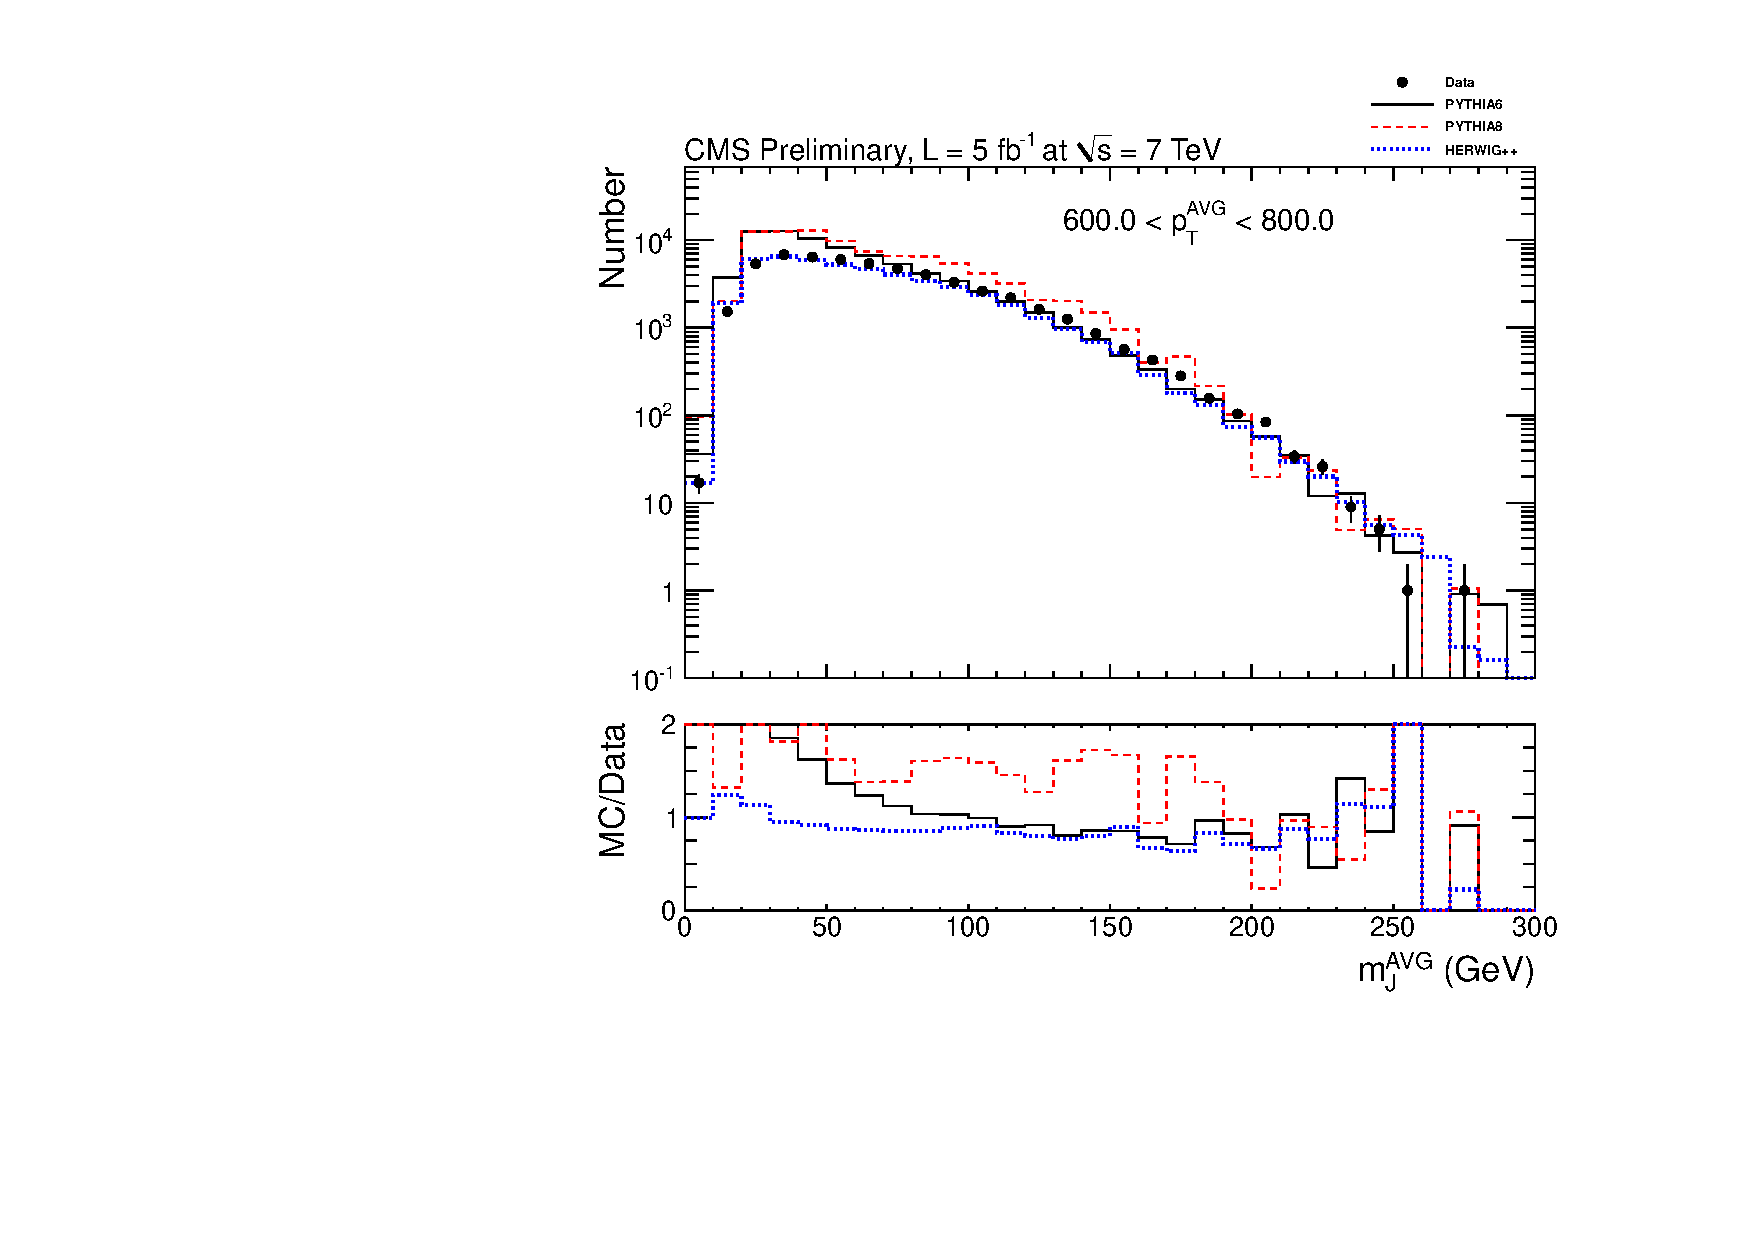
\includegraphics[width=0.95\textwidth]{figs/histAK7MjetVsPtAvg_rawDataMCComparisons_pt_8_Trimmed}
\caption{Detector-level distributions of the jet mass for AK7 Trimmed jets,
for $600.0 < \pt^{AVG} < 800.0$ \GeVc. The data are shown in black points.
The simulated distribution from \PYTHIA is shown in solid black, 
the from \PYTHIAEIGHT in dashed red, and from \HERWIG in dotted blue. 
The bottom frame shows the ratio of the simulated distribution
to the distribution from data. 
\label{figs:histAK7MjetVsPtAvg_rawDataMCComparisons_pt_8_Trimmed}}
\end{figure}



\begin{figure}[htbp]
\centering
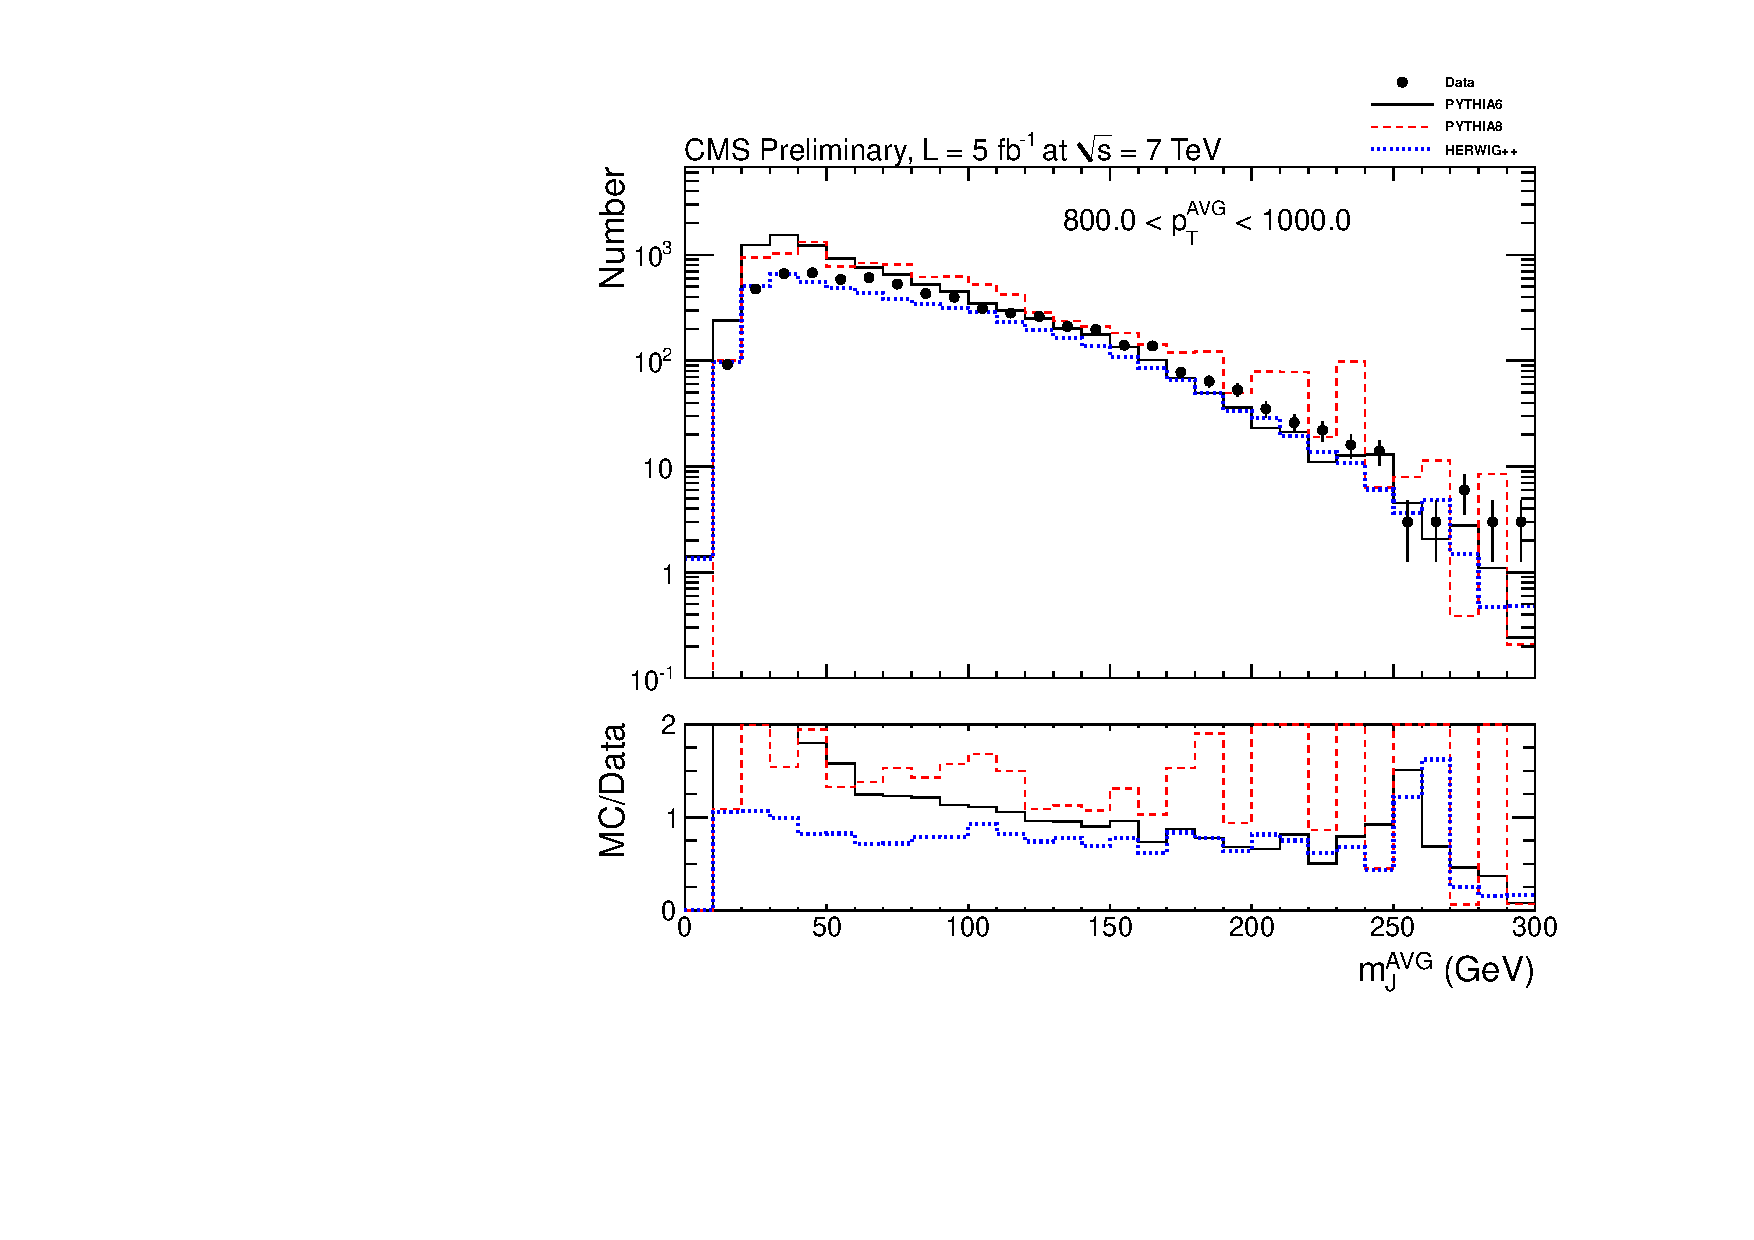
\includegraphics[width=0.95\textwidth]{figs/histAK7MjetVsPtAvg_rawDataMCComparisons_pt_9_Trimmed}
\caption{Detector-level distributions of the jet mass for AK7 Trimmed jets,
for $800.0 < \pt^{AVG} < 1000.0$ \GeVc. The data are shown in black points.
The simulated distribution from \PYTHIA is shown in solid black, 
the from \PYTHIAEIGHT in dashed red, and from \HERWIG in dotted blue. 
The bottom frame shows the ratio of the simulated distribution
to the distribution from data. 
\label{figs:histAK7MjetVsPtAvg_rawDataMCComparisons_pt_9_Trimmed}}
\end{figure}



\begin{figure}[htbp]
\centering
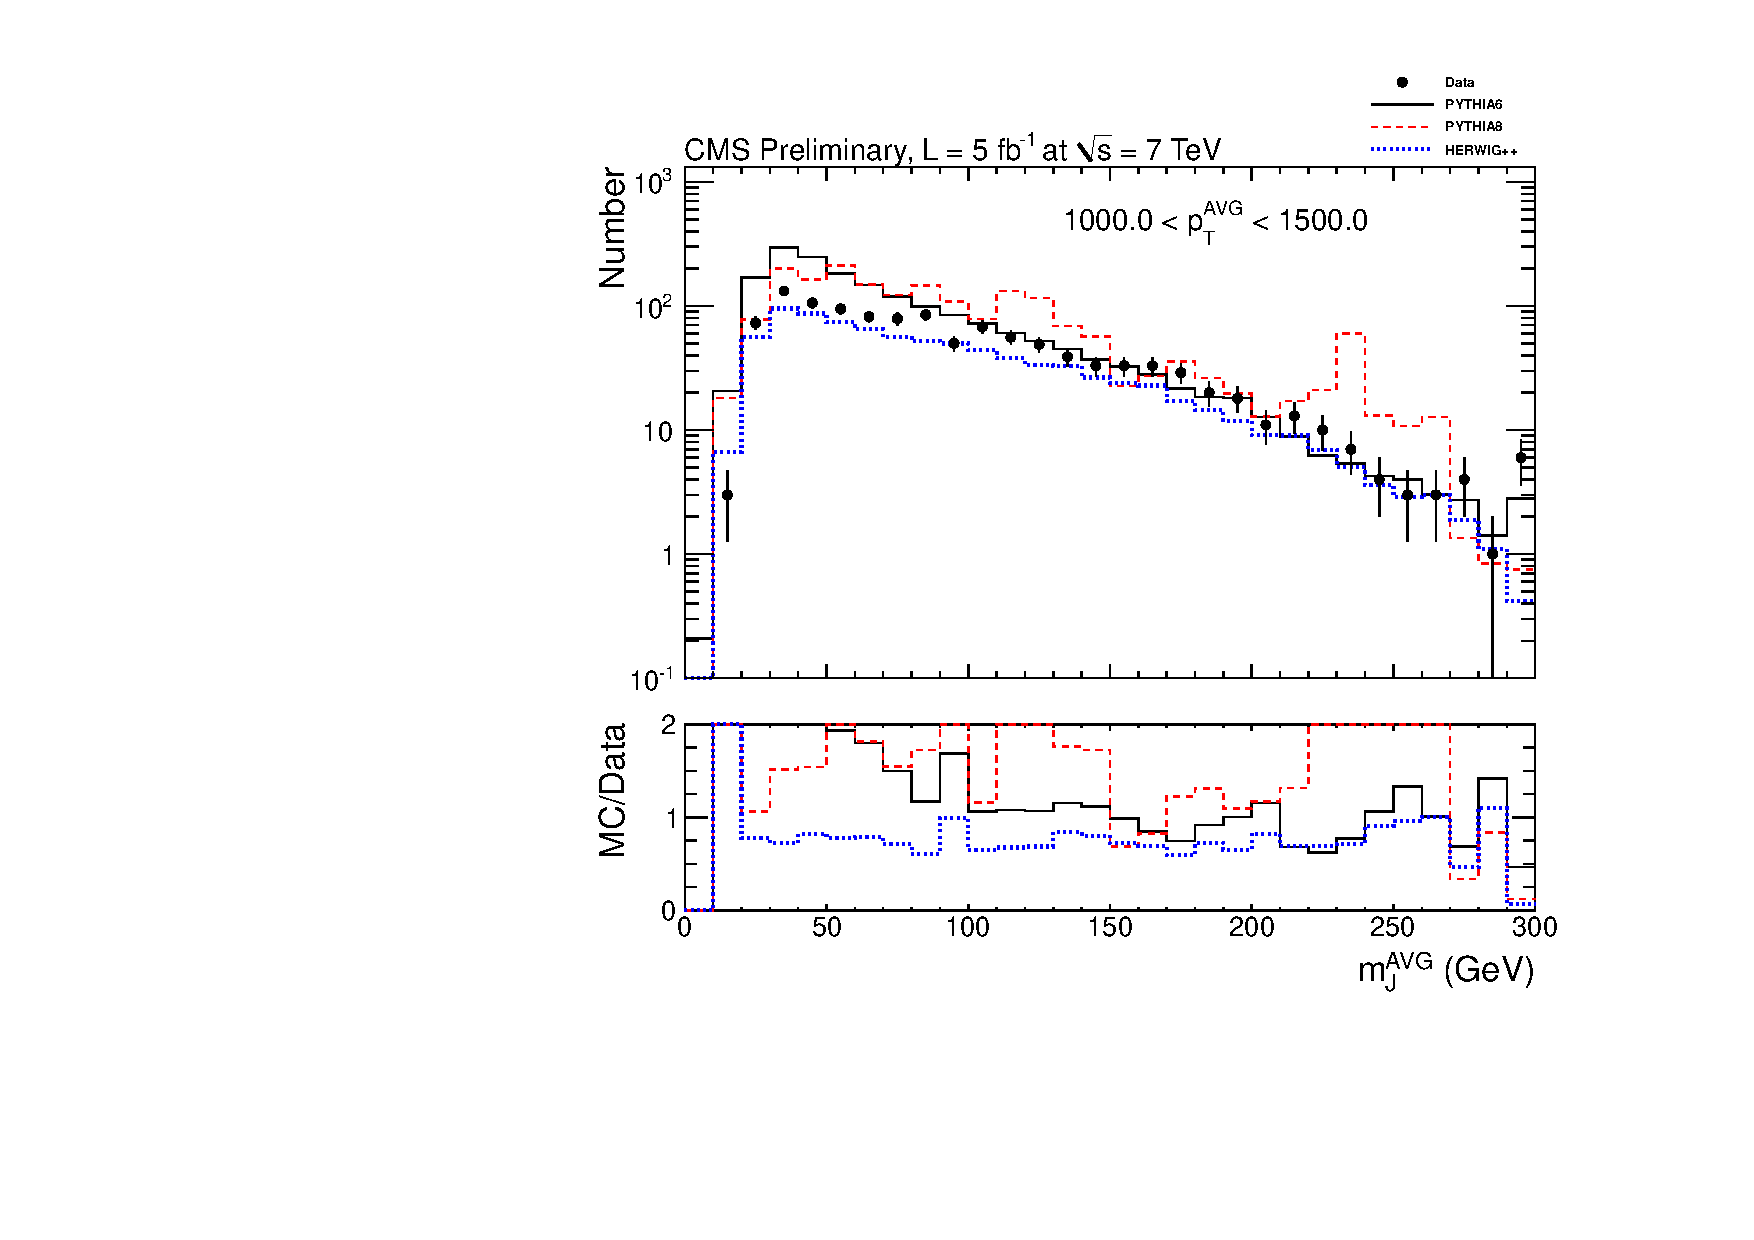
\includegraphics[width=0.95\textwidth]{figs/histAK7MjetVsPtAvg_rawDataMCComparisons_pt_10_Trimmed}
\caption{Detector-level distributions of the jet mass for AK7 Trimmed jets,
for $1000.0 < \pt^{AVG} < 1500.0$ \GeVc. The data are shown in black points.
The simulated distribution from \PYTHIA is shown in solid black, 
the from \PYTHIAEIGHT in dashed red, and from \HERWIG in dotted blue. 
The bottom frame shows the ratio of the simulated distribution
to the distribution from data. 
\label{figs:histAK7MjetVsPtAvg_rawDataMCComparisons_pt_10_Trimmed}}
\end{figure}

\fi

\clearpage

\ifnpas

\begin{figure}[htbp]
\centering
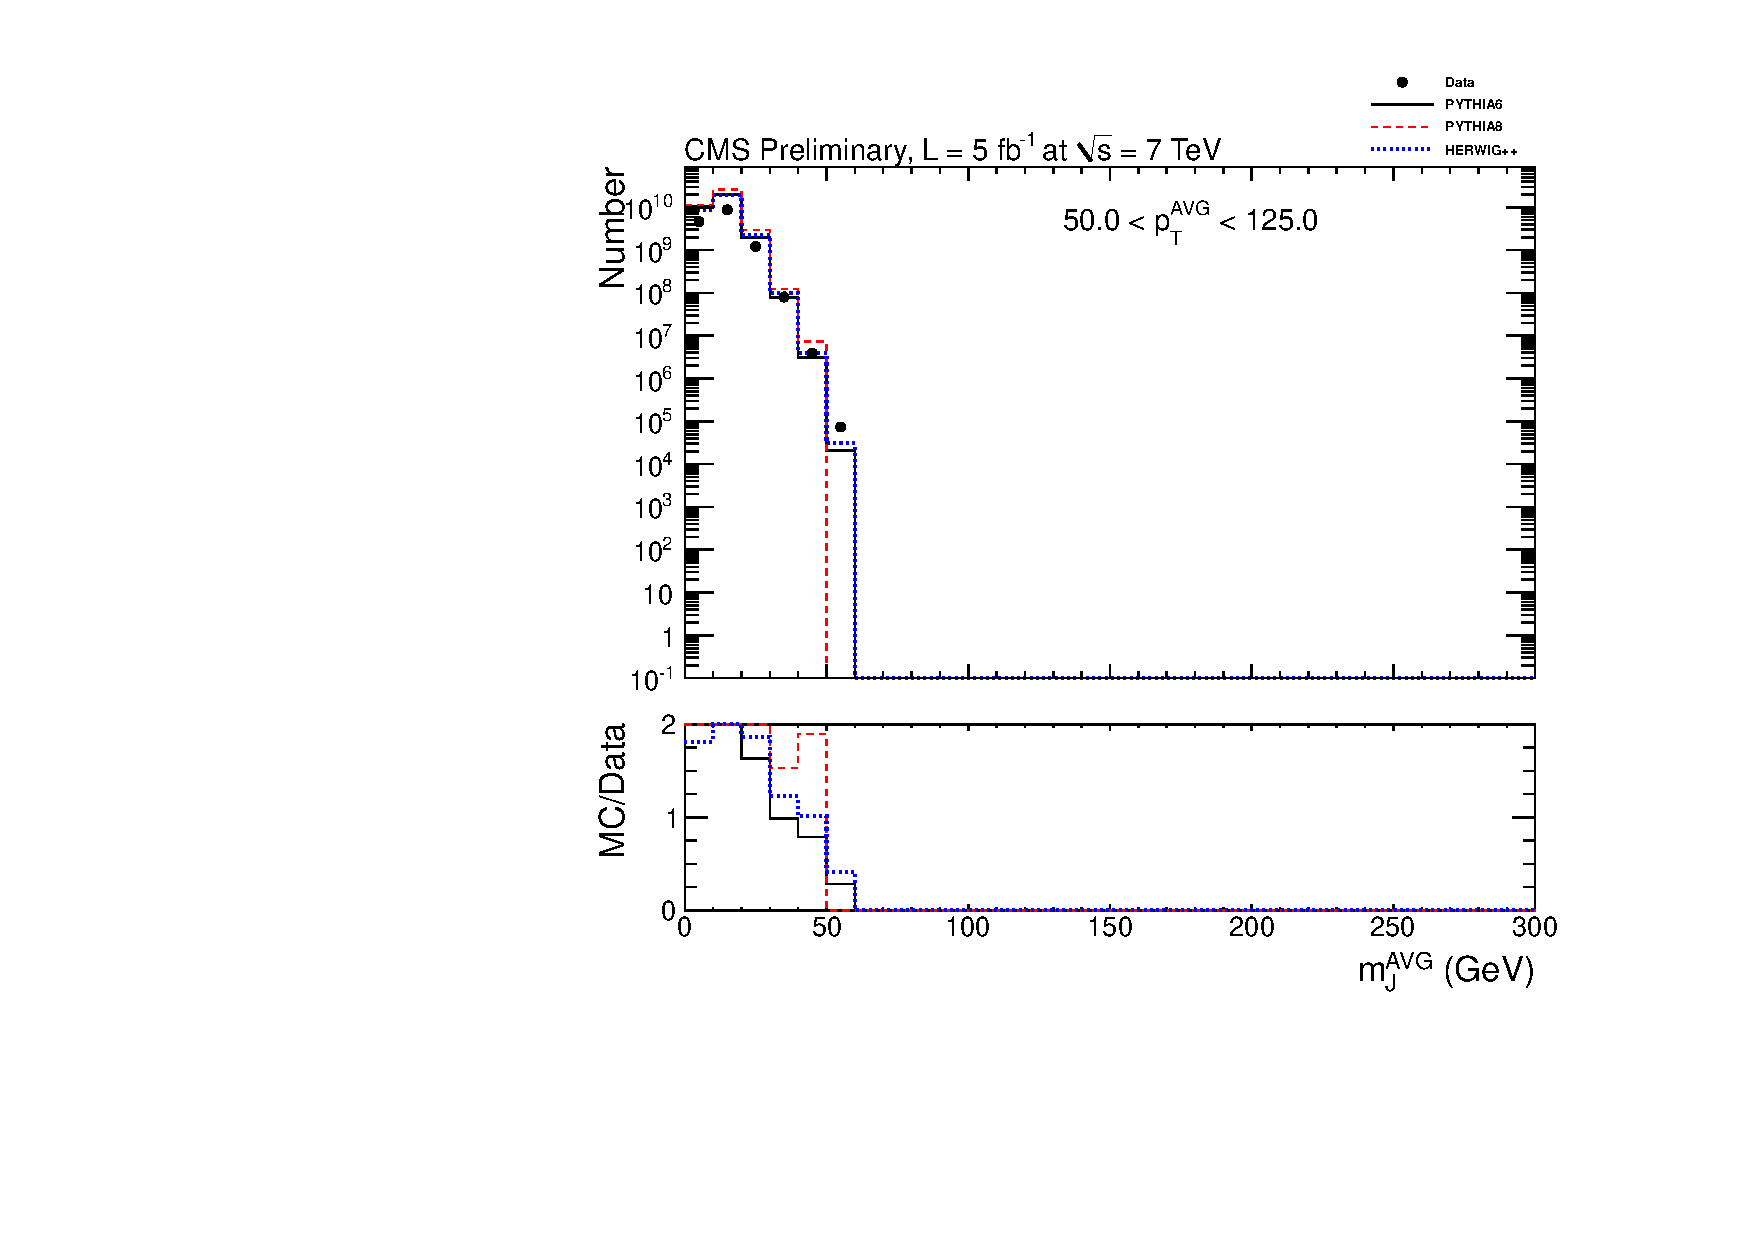
\includegraphics[width=0.95\textwidth]{figs/histAK7MjetVsPtAvg_rawDataMCComparisons_pt_1_Pruned}
\caption{Detector-level distributions of the jet mass for AK7 Pruned jets,
for $50.0 < \pt^{AVG} < 125.0$ \GeVc. The data are shown in black points.
The simulated distribution from \PYTHIA is shown in solid black, 
the from \PYTHIAEIGHT in dashed red, and from \HERWIG in dotted blue. 
The bottom frame shows the ratio of the simulated distribution
to the distribution from data. 
\label{figs:histAK7MjetVsPtAvg_rawDataMCComparisons_pt_1_Pruned}}
\end{figure}

\fi

\begin{figure}[htbp]
\centering
\includegraphics[width=0.49\textwidth]{figs/histAK7MjetVsPtAvg_rawDataMCComparisons_pt_2_Pruned}
\includegraphics[width=0.49\textwidth]{figs/histAK7MjetVsPtAvg_rawDataMCComparisons_pt_3_Pruned}
\includegraphics[width=0.49\textwidth]{figs/histAK7MjetVsPtAvg_rawDataMCComparisons_pt_4_Pruned}
\includegraphics[width=0.49\textwidth]{figs/histAK7MjetVsPtAvg_rawDataMCComparisons_pt_5_Pruned}
\caption{Detector-level distributions of the jet mass for AK7 Pruned jets,
%for $125.0 < \pt^{AVG} < 150.0$ \GeVc. The data are shown in black points.
for several $\pt^{AVG}$ bins. The data are shown in black points.
The simulated distribution from \PYTHIA is shown in solid black, 
the from \PYTHIAEIGHT in dashed red, and from \HERWIG in dotted blue. 
The bottom frame shows the ratio of the simulated distribution
to the distribution from data. 
\label{figs:histAK7MjetVsPtAvg_rawDataMCComparisons_pt_2_Pruned}}
\end{figure}

%%%%%%%%%%
\ifnpas

\begin{figure}[htbp]
\centering
\includegraphics[width=0.95\textwidth]{figs/histAK7MjetVsPtAvg_rawDataMCComparisons_pt_3_Pruned}
\caption{Detector-level distributions of the jet mass for AK7 Pruned jets,
for $150.0 < \pt^{AVG} < 220.0$ \GeVc. The data are shown in black points.
The simulated distribution from \PYTHIA is shown in solid black, 
the from \PYTHIAEIGHT in dashed red, and from \HERWIG in dotted blue. 
The bottom frame shows the ratio of the simulated distribution
to the distribution from data. 
\label{figs:histAK7MjetVsPtAvg_rawDataMCComparisons_pt_3_Pruned}}
\end{figure}



\begin{figure}[htbp]
\centering
\includegraphics[width=0.95\textwidth]{figs/histAK7MjetVsPtAvg_rawDataMCComparisons_pt_4_Pruned}
\caption{Detector-level distributions of the jet mass for AK7 Pruned jets,
for $220.0 < \pt^{AVG} < 300.0$ \GeVc. The data are shown in black points.
The simulated distribution from \PYTHIA is shown in solid black, 
the from \PYTHIAEIGHT in dashed red, and from \HERWIG in dotted blue. 
The bottom frame shows the ratio of the simulated distribution
to the distribution from data. 
\label{figs:histAK7MjetVsPtAvg_rawDataMCComparisons_pt_4_Pruned}}
\end{figure}



\begin{figure}[htbp]
\centering
\includegraphics[width=0.95\textwidth]{figs/histAK7MjetVsPtAvg_rawDataMCComparisons_pt_5_Pruned}
\caption{Detector-level distributions of the jet mass for AK7 Pruned jets,
for $300.0 < \pt^{AVG} < 450.0$ \GeVc. The data are shown in black points.
The simulated distribution from \PYTHIA is shown in solid black, 
the from \PYTHIAEIGHT in dashed red, and from \HERWIG in dotted blue. 
The bottom frame shows the ratio of the simulated distribution
to the distribution from data. 
\label{figs:histAK7MjetVsPtAvg_rawDataMCComparisons_pt_5_Pruned}}
\end{figure}

\fi
%%%%%%%%%%%


\ifnpas

\begin{figure}[htbp]
\centering
\includegraphics[width=0.95\textwidth]{figs/histAK7MjetVsPtAvg_rawDataMCComparisons_pt_6_Pruned}
\caption{Detector-level distributions of the jet mass for AK7 Pruned jets,
for $450.0 < \pt^{AVG} < 500.0$ \GeVc. The data are shown in black points.
The simulated distribution from \PYTHIA is shown in solid black, 
the from \PYTHIAEIGHT in dashed red, and from \HERWIG in dotted blue. 
The bottom frame shows the ratio of the simulated distribution
to the distribution from data. 
\label{figs:histAK7MjetVsPtAvg_rawDataMCComparisons_pt_6_Pruned}}
\end{figure}



\begin{figure}[htbp]
\centering
\includegraphics[width=0.95\textwidth]{figs/histAK7MjetVsPtAvg_rawDataMCComparisons_pt_7_Pruned}
\caption{Detector-level distributions of the jet mass for AK7 Pruned jets,
for $500.0 < \pt^{AVG} < 600.0$ \GeVc. The data are shown in black points.
The simulated distribution from \PYTHIA is shown in solid black, 
the from \PYTHIAEIGHT in dashed red, and from \HERWIG in dotted blue. 
The bottom frame shows the ratio of the simulated distribution
to the distribution from data. 
\label{figs:histAK7MjetVsPtAvg_rawDataMCComparisons_pt_7_Pruned}}
\end{figure}



\begin{figure}[htbp]
\centering
\includegraphics[width=0.95\textwidth]{figs/histAK7MjetVsPtAvg_rawDataMCComparisons_pt_8_Pruned}
\caption{Detector-level distributions of the jet mass for AK7 Pruned jets,
for $600.0 < \pt^{AVG} < 800.0$ \GeVc. The data are shown in black points.
The simulated distribution from \PYTHIA is shown in solid black, 
the from \PYTHIAEIGHT in dashed red, and from \HERWIG in dotted blue. 
The bottom frame shows the ratio of the simulated distribution
to the distribution from data. 
\label{figs:histAK7MjetVsPtAvg_rawDataMCComparisons_pt_8_Pruned}}
\end{figure}



\begin{figure}[htbp]
\centering
\includegraphics[width=0.95\textwidth]{figs/histAK7MjetVsPtAvg_rawDataMCComparisons_pt_9_Pruned}
\caption{Detector-level distributions of the jet mass for AK7 Pruned jets,
for $800.0 < \pt^{AVG} < 1000.0$ \GeVc. The data are shown in black points.
The simulated distribution from \PYTHIA is shown in solid black, 
the from \PYTHIAEIGHT in dashed red, and from \HERWIG in dotted blue. 
The bottom frame shows the ratio of the simulated distribution
to the distribution from data. 
\label{figs:histAK7MjetVsPtAvg_rawDataMCComparisons_pt_9_Pruned}}
\end{figure}



\begin{figure}[htbp]
\centering
\includegraphics[width=0.95\textwidth]{figs/histAK7MjetVsPtAvg_rawDataMCComparisons_pt_10_Pruned}
\caption{Detector-level distributions of the jet mass for AK7 Pruned jets,
for $1000.0 < \pt^{AVG} < 1500.0$ \GeVc. The data are shown in black points.
The simulated distribution from \PYTHIA is shown in solid black, 
the from \PYTHIAEIGHT in dashed red, and from \HERWIG in dotted blue. 
The bottom frame shows the ratio of the simulated distribution
to the distribution from data. 
\label{figs:histAK7MjetVsPtAvg_rawDataMCComparisons_pt_10_Pruned}}
\end{figure}

\fi

\clearpage
